\documentclass[twoside]{book}

% Packages required by doxygen
\usepackage{fixltx2e}
\usepackage{calc}
\usepackage{doxygen}
\usepackage[export]{adjustbox} % also loads graphicx
\usepackage{graphicx}
\usepackage[utf8]{inputenc}
\usepackage{makeidx}
\usepackage{multicol}
\usepackage{multirow}
\PassOptionsToPackage{warn}{textcomp}
\usepackage{textcomp}
\usepackage[nointegrals]{wasysym}
\usepackage[table]{xcolor}

% NLS support packages
\usepackage{hfont}

% Font selection
\usepackage[T1]{fontenc}
\usepackage[scaled=.90]{helvet}
\usepackage{courier}
\usepackage{amssymb}
\usepackage{sectsty}
\renewcommand{\familydefault}{\sfdefault}
\allsectionsfont{%
  \fontseries{bc}\selectfont%
  \color{darkgray}%
}
\renewcommand{\DoxyLabelFont}{%
  \fontseries{bc}\selectfont%
  \color{darkgray}%
}
\newcommand{\+}{\discretionary{\mbox{\scriptsize$\hookleftarrow$}}{}{}}

% Page & text layout
\usepackage{geometry}
\geometry{%
  a4paper,%
  top=2.5cm,%
  bottom=2.5cm,%
  left=2.5cm,%
  right=2.5cm%
}
\tolerance=750
\hfuzz=15pt
\hbadness=750
\setlength{\emergencystretch}{15pt}
\setlength{\parindent}{0cm}
\setlength{\parskip}{3ex plus 2ex minus 2ex}
\makeatletter
\renewcommand{\paragraph}{%
  \@startsection{paragraph}{4}{0ex}{-1.0ex}{1.0ex}{%
    \normalfont\normalsize\bfseries\SS@parafont%
  }%
}
\renewcommand{\subparagraph}{%
  \@startsection{subparagraph}{5}{0ex}{-1.0ex}{1.0ex}{%
    \normalfont\normalsize\bfseries\SS@subparafont%
  }%
}
\makeatother

% Headers & footers
\usepackage{fancyhdr}
\pagestyle{fancyplain}
\fancyhead[LE]{\fancyplain{}{\bfseries\thepage}}
\fancyhead[CE]{\fancyplain{}{}}
\fancyhead[RE]{\fancyplain{}{\bfseries\leftmark}}
\fancyhead[LO]{\fancyplain{}{\bfseries\rightmark}}
\fancyhead[CO]{\fancyplain{}{}}
\fancyhead[RO]{\fancyplain{}{\bfseries\thepage}}
\fancyfoot[LE]{\fancyplain{}{}}
\fancyfoot[CE]{\fancyplain{}{}}
\fancyfoot[RE]{\fancyplain{}{\bfseries\scriptsize 다음에 의해 생성됨 \+:  Doxygen }}
\fancyfoot[LO]{\fancyplain{}{\bfseries\scriptsize 다음에 의해 생성됨 \+:  Doxygen }}
\fancyfoot[CO]{\fancyplain{}{}}
\fancyfoot[RO]{\fancyplain{}{}}
\renewcommand{\footrulewidth}{0.4pt}
\renewcommand{\chaptermark}[1]{%
  \markboth{#1}{}%
}
\renewcommand{\sectionmark}[1]{%
  \markright{\thesection\ #1}%
}

% Indices & bibliography
\usepackage{natbib}
\usepackage[titles]{tocloft}
\setcounter{tocdepth}{3}
\setcounter{secnumdepth}{5}
\makeindex

% Hyperlinks (required, but should be loaded last)
\usepackage{ifpdf}
\ifpdf
  \usepackage[pdftex,pagebackref=true]{hyperref}
\else
  \usepackage[ps2pdf,pagebackref=true]{hyperref}
\fi
\hypersetup{%
  colorlinks=true,%
  linkcolor=blue,%
  citecolor=blue,%
  unicode%
}

% Custom commands
\newcommand{\clearemptydoublepage}{%
  \newpage{\pagestyle{empty}\cleardoublepage}%
}

\usepackage{caption}
\captionsetup{labelsep=space,justification=centering,font={bf},singlelinecheck=off,skip=4pt,position=top}

%===== C O N T E N T S =====

\begin{document}

% Titlepage & ToC
\hypersetup{pageanchor=false,
             bookmarksnumbered=true,
             pdfencoding=unicode
            }
\pagenumbering{alph}
\begin{titlepage}
\vspace*{7cm}
\begin{center}%
{\Large Parking System }\\
\vspace*{1cm}
{\large 다음에 의해 생성됨 \+:  Doxygen 1.8.13}\\
\end{center}
\end{titlepage}
\clearemptydoublepage
\pagenumbering{roman}
\tableofcontents
\clearemptydoublepage
\pagenumbering{arabic}
\hypersetup{pageanchor=true}

%--- Begin generated contents ---
\chapter{Parking System}
\label{index}\hypertarget{index}{}\hypertarget{index_소개}{}\section{소개}\label{index_소개}

\begin{DoxyItemize}
\item 프로젝트 이름 \+: Parking System on Device(\+Raspberry) with Open\+CV Library
\item 
\item 프로젝트 내용 \+: 주차장에 설치된 Camera 에서 얻은 영상 처리하고 기계 학습하여 얻은 정보를 네트워크를 통해 서버와 휴대 전화와 공유한다. -\/$>$처리 순서
\begin{DoxyEnumerate}
\item Camera 로 부터 받은 이미지를 영상 처리
\item 서포트 벡터 머신을 이용하여(\+S\+V\+M) 번호판을 인식
\item 번호판의 좌표를 통해 상대적 좌표를 도출
\item 인경신경망을 이용한 광학 문자 판독기(\+O\+C\+R) 통해 문자 인식
\item 서버 전송
\end{DoxyEnumerate}
\end{DoxyItemize}\hypertarget{index_동작}{}\section{환경}\label{index_동작}

\begin{DoxyItemize}
\item 운영체제 \+: Raspberian
\item 의존성 \+: C++ 11 Open\+CV 3.\+2 이상 Cmake 2.\+8 이상 Open\+MP 
\end{DoxyItemize}\hypertarget{index_src}{}\section{src}\label{index_src}

\begin{DoxyItemize}
\item Network \begin{DoxySeeAlso}{참고}
\hyperlink{_socket_8hpp_source}{Socket.\+hpp} 

\hyperlink{_http_8hpp_source}{Http.\+hpp} 

\hyperlink{ps_a_p_i_8hpp_source}{ps\+A\+P\+I.\+hpp}
\end{DoxySeeAlso}

\item Open\+CV \begin{DoxySeeAlso}{참고}
\hyperlink{_o_c_r_8hpp_source}{O\+C\+R.\+hpp} 

\hyperlink{_plate_8hpp_source}{Plate.\+hpp} 

\hyperlink{process_8hpp_source}{process.\+hpp} 

\hyperlink{_svm_8hpp_source}{Svm.\+hpp} 

\hyperlink{_tools_8hpp_source}{Tools.\+hpp}
\end{DoxySeeAlso}

\item main \begin{DoxySeeAlso}{참고}
\hyperlink{main_8cpp_source}{main.\+cpp} 
\end{DoxySeeAlso}

\end{DoxyItemize}
\chapter{네임스페이스 색인}
\section{네임스페이스 목록}
다음은 문서화된 모든 네임스페이스에 대한 목록입니다. (간략한 설명만을 보여줍니다) \+:\begin{DoxyCompactList}
\item\contentsline{section}{\hyperlink{namespacehttp}{http} \\*H\+T\+TP 메시지를 다루는 네임 스페이스 }{\pageref{namespacehttp}}{}
\item\contentsline{section}{\hyperlink{namespaceprocess}{process} \\*Process 종합적인 진행 namespace }{\pageref{namespaceprocess}}{}
\item\contentsline{section}{\hyperlink{namespaceps}{ps} \\*주차장 관리 시스템 }{\pageref{namespaceps}}{}
\item\contentsline{section}{\hyperlink{namespacesock}{sock} \\*소켓통신을 위한 네임스페이스 }{\pageref{namespacesock}}{}
\item\contentsline{section}{\hyperlink{namespacetools}{tools} \\*Tools 영상 처리 시 유용한 tool 모음 }{\pageref{namespacetools}}{}
\end{DoxyCompactList}

\chapter{계통도 색인}
\section{클래스 계통도}
이 상속 목록은 완전하진 않지만 알파벳순으로 대략적으로 정렬되어있습니다.\+:\begin{DoxyCompactList}
\item \contentsline{section}{tools\+:\+:Analyzer}{\pageref{classtools_1_1_analyzer}}{}
\item \contentsline{section}{ps\+:\+:A\+PI}{\pageref{classps_1_1_a_p_i}}{}
\item \contentsline{section}{tools\+:\+:Dicider}{\pageref{classtools_1_1_dicider}}{}
\item \contentsline{section}{Header\+Line}{\pageref{struct_header_line}}{}
\item \contentsline{section}{Http\+Message}{\pageref{class_http_message}}{}
\begin{DoxyCompactList}
\item \contentsline{section}{Http\+Request\+Messge}{\pageref{class_http_request_messge}}{}
\item \contentsline{section}{Http\+Response\+Messge}{\pageref{class_http_response_messge}}{}
\end{DoxyCompactList}
\item \contentsline{section}{O\+CR}{\pageref{class_o_c_r}}{}
\item \contentsline{section}{O\+C\+R\+Trainer}{\pageref{class_o_c_r_trainer}}{}
\item \contentsline{section}{process\+:\+:Parking\+Info}{\pageref{structprocess_1_1_parking_info}}{}
\item \contentsline{section}{Plate}{\pageref{class_plate}}{}
\item \contentsline{section}{Request\+Line}{\pageref{struct_request_line}}{}
\item \contentsline{section}{Socket}{\pageref{class_socket}}{}
\begin{DoxyCompactList}
\item \contentsline{section}{Client\+Socket}{\pageref{class_client_socket}}{}
\item \contentsline{section}{Server\+Socket}{\pageref{class_server_socket}}{}
\end{DoxyCompactList}
\item \contentsline{section}{Status\+Code}{\pageref{struct_status_code}}{}
\item \contentsline{section}{Svm}{\pageref{class_svm}}{}
\item \contentsline{section}{S\+V\+M\+Trainer}{\pageref{class_s_v_m_trainer}}{}
\item \contentsline{section}{process\+:\+:Table}{\pageref{structprocess_1_1_table}}{}
\item \contentsline{section}{Plate\+:\+:Text}{\pageref{class_plate_1_1_text}}{}
\end{DoxyCompactList}

\chapter{클래스 색인}
\section{클래스 목록}
다음은 클래스, 구조체, 공용체 그리고 인터페이스들입니다. (간략한 설명만을 보여줍니다) \+:\begin{DoxyCompactList}
\item\contentsline{section}{\hyperlink{classtools_1_1_analyzer}{tools\+::\+Analyzer} \\*통계 분석 결과 출력 클래스 입력된 초기 정답 문자열를 영상으로부터 도출된 문자열과 통계적 비교된 결과를 출력한다 }{\pageref{classtools_1_1_analyzer}}{}
\item\contentsline{section}{\hyperlink{classps_1_1_a_p_i}{ps\+::\+A\+PI} }{\pageref{classps_1_1_a_p_i}}{}
\item\contentsline{section}{\hyperlink{class_client_socket}{Client\+Socket} }{\pageref{class_client_socket}}{}
\item\contentsline{section}{\hyperlink{classtools_1_1_dicider}{tools\+::\+Dicider} \\*초기에 입력된 문자열과 비교하여 \hyperlink{classtools_1_1_dicider_afdc1fb561a2ed8037d0fa87b69a7792d}{tools\+::\+Dicider\+::\+L\+E\+A\+S\+T\+M\+A\+T\+CH} 를 넘었을 경우 결과를 도출한다 }{\pageref{classtools_1_1_dicider}}{}
\item\contentsline{section}{\hyperlink{struct_header_line}{Header\+Line} }{\pageref{struct_header_line}}{}
\item\contentsline{section}{\hyperlink{class_http_message}{Http\+Message} }{\pageref{class_http_message}}{}
\item\contentsline{section}{\hyperlink{class_http_request_messge}{Http\+Request\+Messge} }{\pageref{class_http_request_messge}}{}
\item\contentsline{section}{\hyperlink{class_http_response_messge}{Http\+Response\+Messge} }{\pageref{class_http_response_messge}}{}
\item\contentsline{section}{\hyperlink{class_o_c_r}{O\+CR} \\*Artificial Neural Networks을 다루기 위한 클래스 }{\pageref{class_o_c_r}}{}
\item\contentsline{section}{\hyperlink{class_o_c_r_trainer}{O\+C\+R\+Trainer} \\*\hyperlink{class_o_c_r_a9d4b78ff145b1e89ac05eb0f194d1948}{O\+C\+R\+::collect\+Train\+Images} 실행 시 필요한 image를 생성하는 클래스 }{\pageref{class_o_c_r_trainer}}{}
\item\contentsline{section}{\hyperlink{structprocess_1_1_parking_info}{process\+::\+Parking\+Info} \\*주차장 정보 }{\pageref{structprocess_1_1_parking_info}}{}
\item\contentsline{section}{\hyperlink{class_plate}{Plate} \\*번호판 번호판 이미지와 상대적 위치를 포함한 클래스 }{\pageref{class_plate}}{}
\item\contentsline{section}{\hyperlink{struct_request_line}{Request\+Line} }{\pageref{struct_request_line}}{}
\item\contentsline{section}{\hyperlink{class_server_socket}{Server\+Socket} }{\pageref{class_server_socket}}{}
\item\contentsline{section}{\hyperlink{class_socket}{Socket} }{\pageref{class_socket}}{}
\item\contentsline{section}{\hyperlink{struct_status_code}{Status\+Code} }{\pageref{struct_status_code}}{}
\item\contentsline{section}{\hyperlink{class_svm}{Svm} \\*Support Vector Machines을 다루기 위한 클래스 }{\pageref{class_svm}}{}
\item\contentsline{section}{\hyperlink{class_s_v_m_trainer}{S\+V\+M\+Trainer} \\*\hyperlink{class_svm_a1b18e97fffb268f9cfe91152f7e96298}{Svm\+::collect\+Train\+Images} 실행 시 필요한 image를 생성하는 클래스 }{\pageref{class_s_v_m_trainer}}{}
\item\contentsline{section}{\hyperlink{structprocess_1_1_table}{process\+::\+Table} \\*주차 차량 정보 }{\pageref{structprocess_1_1_table}}{}
\item\contentsline{section}{\hyperlink{class_plate_1_1_text}{Plate\+::\+Text} \\*텍스트 번호판을 구성하는 텍스트들 중 하나 }{\pageref{class_plate_1_1_text}}{}
\end{DoxyCompactList}

\chapter{네임스페이스 문서화}
\hypertarget{namespacehttp}{}\section{http 네임스페이스 참조}
\label{namespacehttp}\index{http@{http}}


H\+T\+TP 메시지를 다루는 네임 스페이스  


\subsection*{클래스}
\begin{DoxyCompactItemize}
\item 
struct \hyperlink{structhttp_1_1_header_line}{Header\+Line}
\begin{DoxyCompactList}\small\item\em \hyperlink{classhttp_1_1_message}{Message} 를 구성하는 헤더 \end{DoxyCompactList}\item 
class \hyperlink{classhttp_1_1_message}{Message}
\begin{DoxyCompactList}\small\item\em H\+T\+TP 메세지 \end{DoxyCompactList}\item 
struct \hyperlink{structhttp_1_1_request_line}{Request\+Line}
\begin{DoxyCompactList}\small\item\em \hyperlink{classhttp_1_1_request_messge}{Request\+Messge} 의 요청 라인 \end{DoxyCompactList}\item 
class \hyperlink{classhttp_1_1_request_messge}{Request\+Messge}
\begin{DoxyCompactList}\small\item\em H\+T\+TP 요청 메시지 \end{DoxyCompactList}\item 
class \hyperlink{classhttp_1_1_response_messge}{Response\+Messge}
\begin{DoxyCompactList}\small\item\em H\+T\+TP 응답 메시지 \end{DoxyCompactList}\item 
struct \hyperlink{structhttp_1_1_status_line}{Status\+Line}
\begin{DoxyCompactList}\small\item\em \hyperlink{classhttp_1_1_response_messge}{Response\+Messge} 의 상태 라인 \end{DoxyCompactList}\end{DoxyCompactItemize}


\subsection{상세한 설명}
H\+T\+TP 메시지를 다루는 네임 스페이스 
\hypertarget{namespaceprocess}{}\section{process 네임스페이스 참조}
\label{namespaceprocess}\index{process@{process}}


Process 종합적인 진행 namespace  


\subsection*{클래스}
\begin{DoxyCompactItemize}
\item 
struct \hyperlink{structprocess_1_1_parking_info}{Parking\+Info}
\begin{DoxyCompactList}\small\item\em 주차장 정보 \end{DoxyCompactList}\item 
struct \hyperlink{structprocess_1_1_table}{Table}
\begin{DoxyCompactList}\small\item\em 주차 차량 정보 \end{DoxyCompactList}\end{DoxyCompactItemize}
\subsection*{열거형 타입}
\begin{DoxyCompactItemize}
\item 
enum \hyperlink{namespaceprocess_ac4191f2d90b44ca6a832f36481b403e7}{F\+R\+OM} \{ \hyperlink{namespaceprocess_ac4191f2d90b44ca6a832f36481b403e7a94d429f5a87a63afc443f022bdea773f}{C\+A\+M\+E\+RA} = 0, 
\hyperlink{namespaceprocess_ac4191f2d90b44ca6a832f36481b403e7a4f69e1b61f6a4a73e1473fe711b32837}{F\+I\+L\+E\+S\+Y\+S\+T\+EM} = 1
 \}\begin{DoxyCompactList}\small\item\em image를 입력받을 곳 \end{DoxyCompactList}
\item 
enum \hyperlink{namespaceprocess_aa30669026e4cf69a2550aace23bef68e}{W\+AY} \{ \hyperlink{namespaceprocess_aa30669026e4cf69a2550aace23bef68ea7cc3bc56e3206127aefb779215c3e5f2}{N\+O\+NE} = -\/1, 
\hyperlink{namespaceprocess_aa30669026e4cf69a2550aace23bef68eab1e12dcacd0520703b0da01c19534b34}{E\+N\+T\+ER} = 0, 
\hyperlink{namespaceprocess_aa30669026e4cf69a2550aace23bef68ea3eb2090cfcc0c0999e82591472385128}{E\+X\+IT} = 1
 \}\begin{DoxyCompactList}\small\item\em 카메라 방향 \end{DoxyCompactList}
\item 
enum \hyperlink{namespaceprocess_a38b4d487dfb47b712f32bfa52fa94464}{M\+O\+DE} \{ \newline
\hyperlink{namespaceprocess_a38b4d487dfb47b712f32bfa52fa94464ade7887da7de946a4708baa66f437ce44}{N\+E\+T\+W\+O\+RK} = 0x01, 
\hyperlink{namespaceprocess_a38b4d487dfb47b712f32bfa52fa94464a1997642964991dcd5ee63cd28185ef86}{T\+R\+A\+IN} = 0x02, 
\hyperlink{namespaceprocess_a38b4d487dfb47b712f32bfa52fa94464af1a2ca0ae6e0d4685b3996a47e56c0a6}{P\+O\+S\+I\+T\+I\+ON} = 0x04, 
\hyperlink{namespaceprocess_a38b4d487dfb47b712f32bfa52fa94464ac9d1691ee0c966c08f6cefdd13a27b98}{C\+O\+S\+T\+T\+I\+ME} = 0x08, 
\newline
\hyperlink{namespaceprocess_a38b4d487dfb47b712f32bfa52fa94464a8c488cdfb82009e72ed939d49fbf788e}{P\+L\+A\+T\+E\+S\+TR} = 0x10, 
\hyperlink{namespaceprocess_a38b4d487dfb47b712f32bfa52fa94464a660edf2dffb7ba034fe83e1b28095833}{W\+I\+N\+D\+O\+W\+ON} = 0x20, 
\hyperlink{namespaceprocess_a38b4d487dfb47b712f32bfa52fa94464aa48cdb2d219079ab11a2967b01d7731a}{A\+N\+A\+L\+Y\+S\+IS} = 0x40, 
\hyperlink{namespaceprocess_a38b4d487dfb47b712f32bfa52fa94464a186cfc3bdf8fe842b027d5411b2d0da8}{N\+O\+T\+U\+S\+E\+ML} = 0x80
 \}\begin{DoxyCompactList}\small\item\em 프로그램 Mode \end{DoxyCompactList}
\end{DoxyCompactItemize}
\subsection*{함수}
\begin{DoxyCompactItemize}
\item 
void \hyperlink{namespaceprocess_a1f0aa45cb765ba7d279ac2c2199074ea}{send2\+Server} (const \hyperlink{structprocess_1_1_parking_info}{Parking\+Info} \&info, \hyperlink{structprocess_1_1_table}{Table} table\mbox{[}S\+E\+G\+M\+E\+N\+T\+S\+I\+ZE\mbox{]})
\begin{DoxyCompactList}\small\item\em Server 에게 보내기 \end{DoxyCompactList}\item 
bool \hyperlink{namespaceprocess_a774ab0220f8a28dd0175af9d93fa9dd0}{deduct\+Index} (const cv\+::\+Rect area\mbox{[}S\+E\+G\+M\+E\+N\+T\+S\+I\+ZE\mbox{]}, const cv\+::\+Point \&position, int $\ast$zone\+Index)
\begin{DoxyCompactList}\small\item\em 차량 위치 도출 \end{DoxyCompactList}\item 
int \hyperlink{namespaceprocess_a04e297268dc5195b3c29081e59cb411f}{start\+Opencv} (int width, int height, int mode, \hyperlink{structprocess_1_1_parking_info}{process\+::\+Parking\+Info} info, std\+::string answer)
\begin{DoxyCompactList}\small\item\em Opencv 작업 시작 \end{DoxyCompactList}\end{DoxyCompactItemize}


\subsection{상세한 설명}
Process 종합적인 진행 namespace 

\subsection{열거형 타입 문서화}
\mbox{\Hypertarget{namespaceprocess_ac4191f2d90b44ca6a832f36481b403e7}\label{namespaceprocess_ac4191f2d90b44ca6a832f36481b403e7}} 
\index{process@{process}!F\+R\+OM@{F\+R\+OM}}
\index{F\+R\+OM@{F\+R\+OM}!process@{process}}
\subsubsection{\texorpdfstring{F\+R\+OM}{FROM}}
{\footnotesize\ttfamily enum \hyperlink{namespaceprocess_ac4191f2d90b44ca6a832f36481b403e7}{process\+::\+F\+R\+OM}}



image를 입력받을 곳 

\begin{DoxyEnumFields}{열거형 멤버}
\raisebox{\heightof{T}}[0pt][0pt]{\index{C\+A\+M\+E\+RA@{C\+A\+M\+E\+RA}!process@{process}}\index{process@{process}!C\+A\+M\+E\+RA@{C\+A\+M\+E\+RA}}}\mbox{\Hypertarget{namespaceprocess_ac4191f2d90b44ca6a832f36481b403e7a94d429f5a87a63afc443f022bdea773f}\label{namespaceprocess_ac4191f2d90b44ca6a832f36481b403e7a94d429f5a87a63afc443f022bdea773f}} 
C\+A\+M\+E\+RA&Camera로 부터 \\
\hline

\raisebox{\heightof{T}}[0pt][0pt]{\index{F\+I\+L\+E\+S\+Y\+S\+T\+EM@{F\+I\+L\+E\+S\+Y\+S\+T\+EM}!process@{process}}\index{process@{process}!F\+I\+L\+E\+S\+Y\+S\+T\+EM@{F\+I\+L\+E\+S\+Y\+S\+T\+EM}}}\mbox{\Hypertarget{namespaceprocess_ac4191f2d90b44ca6a832f36481b403e7a4f69e1b61f6a4a73e1473fe711b32837}\label{namespaceprocess_ac4191f2d90b44ca6a832f36481b403e7a4f69e1b61f6a4a73e1473fe711b32837}} 
F\+I\+L\+E\+S\+Y\+S\+T\+EM&File System으로 부터 \\
\hline

\end{DoxyEnumFields}
\mbox{\Hypertarget{namespaceprocess_a38b4d487dfb47b712f32bfa52fa94464}\label{namespaceprocess_a38b4d487dfb47b712f32bfa52fa94464}} 
\index{process@{process}!M\+O\+DE@{M\+O\+DE}}
\index{M\+O\+DE@{M\+O\+DE}!process@{process}}
\subsubsection{\texorpdfstring{M\+O\+DE}{MODE}}
{\footnotesize\ttfamily enum \hyperlink{namespaceprocess_a38b4d487dfb47b712f32bfa52fa94464}{process\+::\+M\+O\+DE}}



프로그램 Mode 

\begin{DoxyEnumFields}{열거형 멤버}
\raisebox{\heightof{T}}[0pt][0pt]{\index{N\+E\+T\+W\+O\+RK@{N\+E\+T\+W\+O\+RK}!process@{process}}\index{process@{process}!N\+E\+T\+W\+O\+RK@{N\+E\+T\+W\+O\+RK}}}\mbox{\Hypertarget{namespaceprocess_a38b4d487dfb47b712f32bfa52fa94464ade7887da7de946a4708baa66f437ce44}\label{namespaceprocess_a38b4d487dfb47b712f32bfa52fa94464ade7887da7de946a4708baa66f437ce44}} 
N\+E\+T\+W\+O\+RK&Network 활성화 \\
\hline

\raisebox{\heightof{T}}[0pt][0pt]{\index{T\+R\+A\+IN@{T\+R\+A\+IN}!process@{process}}\index{process@{process}!T\+R\+A\+IN@{T\+R\+A\+IN}}}\mbox{\Hypertarget{namespaceprocess_a38b4d487dfb47b712f32bfa52fa94464a1997642964991dcd5ee63cd28185ef86}\label{namespaceprocess_a38b4d487dfb47b712f32bfa52fa94464a1997642964991dcd5ee63cd28185ef86}} 
T\+R\+A\+IN&Train 활성화 \\
\hline

\raisebox{\heightof{T}}[0pt][0pt]{\index{P\+O\+S\+I\+T\+I\+ON@{P\+O\+S\+I\+T\+I\+ON}!process@{process}}\index{process@{process}!P\+O\+S\+I\+T\+I\+ON@{P\+O\+S\+I\+T\+I\+ON}}}\mbox{\Hypertarget{namespaceprocess_a38b4d487dfb47b712f32bfa52fa94464af1a2ca0ae6e0d4685b3996a47e56c0a6}\label{namespaceprocess_a38b4d487dfb47b712f32bfa52fa94464af1a2ca0ae6e0d4685b3996a47e56c0a6}} 
P\+O\+S\+I\+T\+I\+ON&Position 표시 \\
\hline

\raisebox{\heightof{T}}[0pt][0pt]{\index{C\+O\+S\+T\+T\+I\+ME@{C\+O\+S\+T\+T\+I\+ME}!process@{process}}\index{process@{process}!C\+O\+S\+T\+T\+I\+ME@{C\+O\+S\+T\+T\+I\+ME}}}\mbox{\Hypertarget{namespaceprocess_a38b4d487dfb47b712f32bfa52fa94464ac9d1691ee0c966c08f6cefdd13a27b98}\label{namespaceprocess_a38b4d487dfb47b712f32bfa52fa94464ac9d1691ee0c966c08f6cefdd13a27b98}} 
C\+O\+S\+T\+T\+I\+ME&소요시간 표시 \\
\hline

\raisebox{\heightof{T}}[0pt][0pt]{\index{P\+L\+A\+T\+E\+S\+TR@{P\+L\+A\+T\+E\+S\+TR}!process@{process}}\index{process@{process}!P\+L\+A\+T\+E\+S\+TR@{P\+L\+A\+T\+E\+S\+TR}}}\mbox{\Hypertarget{namespaceprocess_a38b4d487dfb47b712f32bfa52fa94464a8c488cdfb82009e72ed939d49fbf788e}\label{namespaceprocess_a38b4d487dfb47b712f32bfa52fa94464a8c488cdfb82009e72ed939d49fbf788e}} 
P\+L\+A\+T\+E\+S\+TR&소요시간 표시 \\
\hline

\raisebox{\heightof{T}}[0pt][0pt]{\index{W\+I\+N\+D\+O\+W\+ON@{W\+I\+N\+D\+O\+W\+ON}!process@{process}}\index{process@{process}!W\+I\+N\+D\+O\+W\+ON@{W\+I\+N\+D\+O\+W\+ON}}}\mbox{\Hypertarget{namespaceprocess_a38b4d487dfb47b712f32bfa52fa94464a660edf2dffb7ba034fe83e1b28095833}\label{namespaceprocess_a38b4d487dfb47b712f32bfa52fa94464a660edf2dffb7ba034fe83e1b28095833}} 
W\+I\+N\+D\+O\+W\+ON&각 과정을 Windows로 띄우기 \\
\hline

\raisebox{\heightof{T}}[0pt][0pt]{\index{A\+N\+A\+L\+Y\+S\+IS@{A\+N\+A\+L\+Y\+S\+IS}!process@{process}}\index{process@{process}!A\+N\+A\+L\+Y\+S\+IS@{A\+N\+A\+L\+Y\+S\+IS}}}\mbox{\Hypertarget{namespaceprocess_a38b4d487dfb47b712f32bfa52fa94464aa48cdb2d219079ab11a2967b01d7731a}\label{namespaceprocess_a38b4d487dfb47b712f32bfa52fa94464aa48cdb2d219079ab11a2967b01d7731a}} 
A\+N\+A\+L\+Y\+S\+IS&통계적 계산 측정 \\
\hline

\raisebox{\heightof{T}}[0pt][0pt]{\index{N\+O\+T\+U\+S\+E\+ML@{N\+O\+T\+U\+S\+E\+ML}!process@{process}}\index{process@{process}!N\+O\+T\+U\+S\+E\+ML@{N\+O\+T\+U\+S\+E\+ML}}}\mbox{\Hypertarget{namespaceprocess_a38b4d487dfb47b712f32bfa52fa94464a186cfc3bdf8fe842b027d5411b2d0da8}\label{namespaceprocess_a38b4d487dfb47b712f32bfa52fa94464a186cfc3bdf8fe842b027d5411b2d0da8}} 
N\+O\+T\+U\+S\+E\+ML&인공신경망 사용하지 않기 \\
\hline

\end{DoxyEnumFields}
\mbox{\Hypertarget{namespaceprocess_aa30669026e4cf69a2550aace23bef68e}\label{namespaceprocess_aa30669026e4cf69a2550aace23bef68e}} 
\index{process@{process}!W\+AY@{W\+AY}}
\index{W\+AY@{W\+AY}!process@{process}}
\subsubsection{\texorpdfstring{W\+AY}{WAY}}
{\footnotesize\ttfamily enum \hyperlink{namespaceprocess_aa30669026e4cf69a2550aace23bef68e}{process\+::\+W\+AY}}



카메라 방향 

\begin{DoxyEnumFields}{열거형 멤버}
\raisebox{\heightof{T}}[0pt][0pt]{\index{N\+O\+NE@{N\+O\+NE}!process@{process}}\index{process@{process}!N\+O\+NE@{N\+O\+NE}}}\mbox{\Hypertarget{namespaceprocess_aa30669026e4cf69a2550aace23bef68ea7cc3bc56e3206127aefb779215c3e5f2}\label{namespaceprocess_aa30669026e4cf69a2550aace23bef68ea7cc3bc56e3206127aefb779215c3e5f2}} 
N\+O\+NE&N\+O\+NE \\
\hline

\raisebox{\heightof{T}}[0pt][0pt]{\index{E\+N\+T\+ER@{E\+N\+T\+ER}!process@{process}}\index{process@{process}!E\+N\+T\+ER@{E\+N\+T\+ER}}}\mbox{\Hypertarget{namespaceprocess_aa30669026e4cf69a2550aace23bef68eab1e12dcacd0520703b0da01c19534b34}\label{namespaceprocess_aa30669026e4cf69a2550aace23bef68eab1e12dcacd0520703b0da01c19534b34}} 
E\+N\+T\+ER&입구 \\
\hline

\raisebox{\heightof{T}}[0pt][0pt]{\index{E\+X\+IT@{E\+X\+IT}!process@{process}}\index{process@{process}!E\+X\+IT@{E\+X\+IT}}}\mbox{\Hypertarget{namespaceprocess_aa30669026e4cf69a2550aace23bef68ea3eb2090cfcc0c0999e82591472385128}\label{namespaceprocess_aa30669026e4cf69a2550aace23bef68ea3eb2090cfcc0c0999e82591472385128}} 
E\+X\+IT&출구 \\
\hline

\end{DoxyEnumFields}


\subsection{함수 문서화}
\mbox{\Hypertarget{namespaceprocess_a774ab0220f8a28dd0175af9d93fa9dd0}\label{namespaceprocess_a774ab0220f8a28dd0175af9d93fa9dd0}} 
\index{process@{process}!deduct\+Index@{deduct\+Index}}
\index{deduct\+Index@{deduct\+Index}!process@{process}}
\subsubsection{\texorpdfstring{deduct\+Index()}{deductIndex()}}
{\footnotesize\ttfamily bool process\+::deduct\+Index (\begin{DoxyParamCaption}\item[{const cv\+::\+Rect}]{area\mbox{[}\+S\+E\+G\+M\+E\+N\+T\+S\+I\+Z\+E\mbox{]},  }\item[{const cv\+::\+Point \&}]{position,  }\item[{int $\ast$}]{zone\+Index }\end{DoxyParamCaption})}



차량 위치 도출 


\begin{DoxyParams}{매개변수}
{\em area} & S\+E\+G\+M\+E\+N\+T\+S\+I\+ZE 개수로 나뉘어진 사각형 영역 \\
\hline
{\em position} & 번호판의 좌표 \\
\hline
{\em zone\+Index} & 도출된 차량 위치 \\
\hline
\end{DoxyParams}
\begin{DoxyReturn}{반환값}
해당하는 위치가 존재하면 true 그렇지 않으면 false position이 각각의 area 중에 포함되는지 검사한다. 
\end{DoxyReturn}
\mbox{\Hypertarget{namespaceprocess_a1f0aa45cb765ba7d279ac2c2199074ea}\label{namespaceprocess_a1f0aa45cb765ba7d279ac2c2199074ea}} 
\index{process@{process}!send2\+Server@{send2\+Server}}
\index{send2\+Server@{send2\+Server}!process@{process}}
\subsubsection{\texorpdfstring{send2\+Server()}{send2Server()}}
{\footnotesize\ttfamily void process\+::send2\+Server (\begin{DoxyParamCaption}\item[{const \hyperlink{structprocess_1_1_parking_info}{Parking\+Info} \&}]{info,  }\item[{\hyperlink{structprocess_1_1_table}{Table}}]{table\mbox{[}\+S\+E\+G\+M\+E\+N\+T\+S\+I\+Z\+E\mbox{]} }\end{DoxyParamCaption})}



Server 에게 보내기 


\begin{DoxyParams}{매개변수}
{\em info} & 주차장 정보 \\
\hline
{\em table} & 주차 차량 정보 \\
\hline
\end{DoxyParams}
\mbox{\Hypertarget{namespaceprocess_a04e297268dc5195b3c29081e59cb411f}\label{namespaceprocess_a04e297268dc5195b3c29081e59cb411f}} 
\index{process@{process}!start\+Opencv@{start\+Opencv}}
\index{start\+Opencv@{start\+Opencv}!process@{process}}
\subsubsection{\texorpdfstring{start\+Opencv()}{startOpencv()}}
{\footnotesize\ttfamily int process\+::start\+Opencv (\begin{DoxyParamCaption}\item[{int}]{width,  }\item[{int}]{height,  }\item[{int}]{mode,  }\item[{\hyperlink{structprocess_1_1_parking_info}{process\+::\+Parking\+Info}}]{info,  }\item[{std\+::string}]{answer }\end{DoxyParamCaption})}



Opencv 작업 시작 


\begin{DoxyParams}{매개변수}
{\em width} & 영상 처리할 이미지의 가로 길이 \\
\hline
{\em height} & 영상 처리할 이미지의 세로 길이 \\
\hline
{\em mode} & 영상 처리에 대한 모드 \\
\hline
{\em info} & 주차 차량 정보 \\
\hline
{\em answer} & 통계 정보 또는 결과물을 훈련 데이터에 저장하기 위한 정답 \\
\hline
\end{DoxyParams}
\begin{DoxySeeAlso}{참고}
\hyperlink{class_o_c_r_trainer}{O\+C\+R\+Trainer} 
\end{DoxySeeAlso}
Camera 열기

주차 영역

Open\+MP Thread 생성

Camera image 불러오는 Thread

Svm을 통해 번호판 여부 확인 
\hypertarget{namespaceps}{}\section{ps 네임스페이스 참조}
\label{namespaceps}\index{ps@{ps}}


주차장 관리 시스템  


\subsection*{클래스}
\begin{DoxyCompactItemize}
\item 
class \hyperlink{classps_1_1_a_p_i}{A\+PI}
\begin{DoxyCompactList}\small\item\em 주차장의 차량 정보를 서버와 통신하기 위한 api \end{DoxyCompactList}\end{DoxyCompactItemize}


\subsection{상세한 설명}
주차장 관리 시스템 
\hypertarget{namespacesock}{}\section{sock 네임스페이스 참조}
\label{namespacesock}\index{sock@{sock}}


소켓통신을 위한 네임스페이스  


\subsection*{클래스}
\begin{DoxyCompactItemize}
\item 
class \hyperlink{classsock_1_1_client_socket}{Client\+Socket}
\begin{DoxyCompactList}\small\item\em 클라이언트 소켓 \end{DoxyCompactList}\item 
class \hyperlink{classsock_1_1_server_socket}{Server\+Socket}
\begin{DoxyCompactList}\small\item\em 서버 소켓 \end{DoxyCompactList}\item 
class \hyperlink{classsock_1_1_socket}{Socket}
\begin{DoxyCompactList}\small\item\em 소켓 클래스 \end{DoxyCompactList}\end{DoxyCompactItemize}


\subsection{상세한 설명}
소켓통신을 위한 네임스페이스 
\hypertarget{namespacetools}{}\section{tools 네임스페이스 참조}
\label{namespacetools}\index{tools@{tools}}


tools 영상 처리 시 유용한 tool 모음  


\subsection*{클래스}
\begin{DoxyCompactItemize}
\item 
class \hyperlink{classtools_1_1_analyzer}{Analyzer}
\begin{DoxyCompactList}\small\item\em 통계 분석 결과 출력 클래스 입력된 초기 정답 문자열를 영상으로부터 도출된 문자열과 통계적 비교된 결과를 출력한다. \end{DoxyCompactList}\item 
class \hyperlink{classtools_1_1_dicider}{Dicider}
\begin{DoxyCompactList}\small\item\em 초기에 입력된 문자열과 비교하여 \hyperlink{classtools_1_1_dicider_afdc1fb561a2ed8037d0fa87b69a7792d}{tools\+::\+Dicider\+::\+L\+E\+A\+S\+T\+M\+A\+T\+CH} 를 넘었을 경우 결과를 도출한다. \end{DoxyCompactList}\end{DoxyCompactItemize}
\subsection*{함수}
\begin{DoxyCompactItemize}
\item 
bool \hyperlink{namespacetools_a0dabcdc87de76f44797f16ade56944cf}{read\+Image} (const std\+::string fn, cv\+::\+Mat \&image, int flags=1)
\begin{DoxyCompactList}\small\item\em File System으로 부터 이미지 불러오기 \end{DoxyCompactList}\item 
bool \hyperlink{namespacetools_a22a0c0860e714d4b350f17ec02ec2b6b}{write\+Image} (const std\+::string fn, const cv\+::\+Mat \&image)
\begin{DoxyCompactList}\small\item\em File System으로 Image를 쓰기 \end{DoxyCompactList}\end{DoxyCompactItemize}


\subsection{상세한 설명}
tools 영상 처리 시 유용한 tool 모음 

\subsection{함수 문서화}
\mbox{\Hypertarget{namespacetools_a0dabcdc87de76f44797f16ade56944cf}\label{namespacetools_a0dabcdc87de76f44797f16ade56944cf}} 
\index{tools@{tools}!read\+Image@{read\+Image}}
\index{read\+Image@{read\+Image}!tools@{tools}}
\subsubsection{\texorpdfstring{read\+Image()}{readImage()}}
{\footnotesize\ttfamily bool tools\+::read\+Image (\begin{DoxyParamCaption}\item[{const std\+::string}]{fn,  }\item[{cv\+::\+Mat \&}]{image,  }\item[{int}]{flags = {\ttfamily 1} }\end{DoxyParamCaption})}



File System으로 부터 이미지 불러오기 


\begin{DoxyParams}{매개변수}
{\em fn} & 이미지 파일 경로 \\
\hline
{\em image} & File System에서 불러온 이미지를 저장할 변수 \\
\hline
{\em flags} & cv\+::\+Imread\+Modes 의 값을 지정 \\
\hline
\end{DoxyParams}
\begin{DoxyReturn}{반환값}
성공 시 true 그렇지 않으면 false 
\end{DoxyReturn}
\mbox{\Hypertarget{namespacetools_a22a0c0860e714d4b350f17ec02ec2b6b}\label{namespacetools_a22a0c0860e714d4b350f17ec02ec2b6b}} 
\index{tools@{tools}!write\+Image@{write\+Image}}
\index{write\+Image@{write\+Image}!tools@{tools}}
\subsubsection{\texorpdfstring{write\+Image()}{writeImage()}}
{\footnotesize\ttfamily bool tools\+::write\+Image (\begin{DoxyParamCaption}\item[{const std\+::string}]{fn,  }\item[{const cv\+::\+Mat \&}]{image }\end{DoxyParamCaption})}



File System으로 Image를 쓰기 


\begin{DoxyParams}{매개변수}
{\em fn} & 이미지 파일 경로 \\
\hline
{\em image} & File System에 쓸 이미지 변수 \\
\hline
\end{DoxyParams}
\begin{DoxyReturn}{반환값}
성공 시 true 그렇지 않으면 false 
\end{DoxyReturn}

\chapter{클래스 문서화}
\hypertarget{classtools_1_1_analyzer}{}\section{tools\+:\+:Analyzer 클래스 참조}
\label{classtools_1_1_analyzer}\index{tools\+::\+Analyzer@{tools\+::\+Analyzer}}


통계 분석 결과 출력 클래스 입력된 초기 정답 문자열를 영상으로부터 도출된 문자열과 통계적 비교된 결과를 출력한다.  




{\ttfamily \#include $<$Tools.\+hpp$>$}

\subsection*{Public 멤버 함수}
\begin{DoxyCompactItemize}
\item 
\hyperlink{classtools_1_1_analyzer_a6510bc1e10d40e671db16b7a91fc8fac}{Analyzer} (const std\+::string \hyperlink{classtools_1_1_analyzer_a266409271441e355f817ffe0ffd59250}{answer})
\begin{DoxyCompactList}\small\item\em \hyperlink{classtools_1_1_analyzer}{Analyzer} 초기화 \end{DoxyCompactList}\item 
void \hyperlink{classtools_1_1_analyzer_abd1e57e10b843dca874e933236363efa}{analyze} (const std\+::string str)
\begin{DoxyCompactList}\small\item\em 입력받은 문자열을 정답과 비교하며 통계적 계산 결과를 출력 \end{DoxyCompactList}\end{DoxyCompactItemize}
\subsection*{Private 속성}
\begin{DoxyCompactItemize}
\item 
\mbox{\Hypertarget{classtools_1_1_analyzer_a8a38c47fc2d716a805f026dea1ea2868}\label{classtools_1_1_analyzer_a8a38c47fc2d716a805f026dea1ea2868}} 
int \hyperlink{classtools_1_1_analyzer_a8a38c47fc2d716a805f026dea1ea2868}{total\+Correct}
\begin{DoxyCompactList}\small\item\em 총 맞은 횟수 \end{DoxyCompactList}\item 
\mbox{\Hypertarget{classtools_1_1_analyzer_a3e378819a8a7d97b4cffb83cd2cde912}\label{classtools_1_1_analyzer_a3e378819a8a7d97b4cffb83cd2cde912}} 
int \hyperlink{classtools_1_1_analyzer_a3e378819a8a7d97b4cffb83cd2cde912}{total\+Try}
\begin{DoxyCompactList}\small\item\em 총 시도한 횟수 \end{DoxyCompactList}\item 
\mbox{\Hypertarget{classtools_1_1_analyzer_a266409271441e355f817ffe0ffd59250}\label{classtools_1_1_analyzer_a266409271441e355f817ffe0ffd59250}} 
std\+::string \hyperlink{classtools_1_1_analyzer_a266409271441e355f817ffe0ffd59250}{answer}
\begin{DoxyCompactList}\small\item\em 비교할 정답 \end{DoxyCompactList}\end{DoxyCompactItemize}


\subsection{상세한 설명}
통계 분석 결과 출력 클래스 입력된 초기 정답 문자열를 영상으로부터 도출된 문자열과 통계적 비교된 결과를 출력한다. 

Tools.\+hpp 파일의 60 번째 라인에서 정의되었습니다.



\subsection{생성자 \& 소멸자 문서화}
\mbox{\Hypertarget{classtools_1_1_analyzer_a6510bc1e10d40e671db16b7a91fc8fac}\label{classtools_1_1_analyzer_a6510bc1e10d40e671db16b7a91fc8fac}} 
\index{tools\+::\+Analyzer@{tools\+::\+Analyzer}!Analyzer@{Analyzer}}
\index{Analyzer@{Analyzer}!tools\+::\+Analyzer@{tools\+::\+Analyzer}}
\subsubsection{\texorpdfstring{Analyzer()}{Analyzer()}}
{\footnotesize\ttfamily tools\+::\+Analyzer\+::\+Analyzer (\begin{DoxyParamCaption}\item[{const std\+::string}]{answer }\end{DoxyParamCaption})}



\hyperlink{classtools_1_1_analyzer}{Analyzer} 초기화 


\begin{DoxyParams}{매개변수}
{\em answer} & 정답을 설정 \\
\hline
\end{DoxyParams}


Tools.\+cpp 파일의 37 번째 라인에서 정의되었습니다.



\subsection{멤버 함수 문서화}
\mbox{\Hypertarget{classtools_1_1_analyzer_abd1e57e10b843dca874e933236363efa}\label{classtools_1_1_analyzer_abd1e57e10b843dca874e933236363efa}} 
\index{tools\+::\+Analyzer@{tools\+::\+Analyzer}!analyze@{analyze}}
\index{analyze@{analyze}!tools\+::\+Analyzer@{tools\+::\+Analyzer}}
\subsubsection{\texorpdfstring{analyze()}{analyze()}}
{\footnotesize\ttfamily void tools\+::\+Analyzer\+::analyze (\begin{DoxyParamCaption}\item[{const std\+::string}]{str }\end{DoxyParamCaption})}



입력받은 문자열을 정답과 비교하며 통계적 계산 결과를 출력 


\begin{DoxyParams}{매개변수}
{\em str} & 정답과 비교할 문자열 \\
\hline
\end{DoxyParams}


Tools.\+cpp 파일의 43 번째 라인에서 정의되었습니다.



이 클래스에 대한 문서화 페이지는 다음의 파일들로부터 생성되었습니다.\+:\begin{DoxyCompactItemize}
\item 
Opencv/Tools.\+hpp\item 
Opencv/Tools.\+cpp\end{DoxyCompactItemize}

\hypertarget{classps_1_1_a_p_i}{}\section{ps\+:\+:A\+PI 클래스 참조}
\label{classps_1_1_a_p_i}\index{ps\+::\+A\+PI@{ps\+::\+A\+PI}}


주차장의 차량 정보를 서버와 통신하기 위한 api  




{\ttfamily \#include $<$ps\+A\+P\+I.\+hpp$>$}

\subsection*{Public 멤버 함수}
\begin{DoxyCompactItemize}
\item 
\hyperlink{classps_1_1_a_p_i_aecd75588093e5e2dbb9b889ec2162b37}{A\+PI} (std\+::string \hyperlink{classps_1_1_a_p_i_a0d5f99f63a0697e0764f3ee9794a5c26}{hostname}, int \hyperlink{classps_1_1_a_p_i_a58739732fd3c99f9725e5e1376bd5dd7}{port})
\begin{DoxyCompactList}\small\item\em \hyperlink{classps_1_1_a_p_i}{A\+PI} 클래스를 초기화하는 생성자 \end{DoxyCompactList}\item 
void \hyperlink{classps_1_1_a_p_i_a1b8af0de54794775c106e3e68fbe24a6}{inout} (std\+::string plate\+Str, std\+::string inout)
\begin{DoxyCompactList}\small\item\em 주차장에 차량 출입시에 번호판 텍스트를 서버에 보내는 메소드 \end{DoxyCompactList}\item 
void \hyperlink{classps_1_1_a_p_i_a4d7bcb7036c05867179a9a199862f192}{enter} (std\+::string plate\+Str)
\begin{DoxyCompactList}\small\item\em 주차장에 들어오는 차량의 번호판 텍스트를 서버에 보내는 메소드 \end{DoxyCompactList}\item 
void \hyperlink{classps_1_1_a_p_i_ae8af546ae3b183fec0c6d3f68a7e9649}{exit} (std\+::string plate\+Str)
\begin{DoxyCompactList}\small\item\em 주차장을 나가는 차량의 번호판 텍스트를 서버에 보내는 메소드 \end{DoxyCompactList}\item 
void \hyperlink{classps_1_1_a_p_i_af7829fef44876d076e41f18e9978609e}{parking} (int floor, std\+::string zone\+Name, int zone\+Index, std\+::string plate\+Str)
\begin{DoxyCompactList}\small\item\em 주차 시 주차 정보를 서버에 보내는 메소드 \end{DoxyCompactList}\item 
\mbox{\Hypertarget{classps_1_1_a_p_i_a394416393e2ad3bee0141213bbb912a5}\label{classps_1_1_a_p_i_a394416393e2ad3bee0141213bbb912a5}} 
bool \hyperlink{classps_1_1_a_p_i_a394416393e2ad3bee0141213bbb912a5}{resopnse} ()
\begin{DoxyCompactList}\small\item\em 서버에 보낸 메시지에 대한 응답를 html 문서로 내보내는 메소드 \end{DoxyCompactList}\item 
\mbox{\Hypertarget{classps_1_1_a_p_i_a95079fba53baabfafc37e52a6019ba02}\label{classps_1_1_a_p_i_a95079fba53baabfafc37e52a6019ba02}} 
void {\bfseries enter} (string str)
\item 
\mbox{\Hypertarget{classps_1_1_a_p_i_a3d5c8c0fbc56d5dc664e5c0e6747f4f4}\label{classps_1_1_a_p_i_a3d5c8c0fbc56d5dc664e5c0e6747f4f4}} 
void {\bfseries exit} (string str)
\item 
\mbox{\Hypertarget{classps_1_1_a_p_i_a7d7ef9bf708cb009945fcf3b7064977f}\label{classps_1_1_a_p_i_a7d7ef9bf708cb009945fcf3b7064977f}} 
void {\bfseries parking} (int floor, string zone\+Name, int i, string str)
\item 
\mbox{\Hypertarget{classps_1_1_a_p_i_a248e7f4b193ec8c5eb5adfa408e50779}\label{classps_1_1_a_p_i_a248e7f4b193ec8c5eb5adfa408e50779}} 
void {\bfseries resopnse} ()
\end{DoxyCompactItemize}
\subsection*{Private 멤버 함수}
\begin{DoxyCompactItemize}
\item 
void \hyperlink{classps_1_1_a_p_i_a5e11883deb21d5638fabbc7569f9f44f}{set\+Header} (\hyperlink{structhttp_1_1_header_line}{http\+::\+Header\+Line} header\+Line\mbox{[}$\,$\mbox{]}, std\+::string content)
\begin{DoxyCompactList}\small\item\em 서버에 보낼 H\+T\+TP 메세지의 헤더를 정의하는 메소드 \end{DoxyCompactList}\end{DoxyCompactItemize}
\subsection*{Private 속성}
\begin{DoxyCompactItemize}
\item 
\mbox{\Hypertarget{classps_1_1_a_p_i_ad2fc70fe286d0f2eba61b610e2b303df}\label{classps_1_1_a_p_i_ad2fc70fe286d0f2eba61b610e2b303df}} 
int \hyperlink{classps_1_1_a_p_i_ad2fc70fe286d0f2eba61b610e2b303df}{H\+E\+A\+D\+E\+R\+S\+I\+ZE} = 8
\begin{DoxyCompactList}\small\item\em 서버에 보낼 H\+T\+TP 메세지의 헤더의 갯수 \end{DoxyCompactList}\item 
\mbox{\Hypertarget{classps_1_1_a_p_i_a58739732fd3c99f9725e5e1376bd5dd7}\label{classps_1_1_a_p_i_a58739732fd3c99f9725e5e1376bd5dd7}} 
int \hyperlink{classps_1_1_a_p_i_a58739732fd3c99f9725e5e1376bd5dd7}{port}
\begin{DoxyCompactList}\small\item\em 서버 포트 번호 \end{DoxyCompactList}\item 
\mbox{\Hypertarget{classps_1_1_a_p_i_a0d5f99f63a0697e0764f3ee9794a5c26}\label{classps_1_1_a_p_i_a0d5f99f63a0697e0764f3ee9794a5c26}} 
std\+::string \hyperlink{classps_1_1_a_p_i_a0d5f99f63a0697e0764f3ee9794a5c26}{hostname}
\begin{DoxyCompactList}\small\item\em 서버 호스트 이름 \end{DoxyCompactList}\item 
\mbox{\Hypertarget{classps_1_1_a_p_i_ae93da803b67097f16a009d7acf78d957}\label{classps_1_1_a_p_i_ae93da803b67097f16a009d7acf78d957}} 
std\+::string \hyperlink{classps_1_1_a_p_i_ae93da803b67097f16a009d7acf78d957}{path}
\begin{DoxyCompactList}\small\item\em H\+T\+ML 문서를 저장할 경로 \end{DoxyCompactList}\item 
\mbox{\Hypertarget{classps_1_1_a_p_i_af262de65cbf1ede5881c3c75d3cca049}\label{classps_1_1_a_p_i_af262de65cbf1ede5881c3c75d3cca049}} 
\hyperlink{classsock_1_1_client_socket}{sock\+::\+Client\+Socket} $\ast$ \hyperlink{classps_1_1_a_p_i_af262de65cbf1ede5881c3c75d3cca049}{sock}
\begin{DoxyCompactList}\small\item\em 서버 소켓 \end{DoxyCompactList}\item 
\mbox{\Hypertarget{classps_1_1_a_p_i_a592e8c7a71b12ae09e28588b4b687fe9}\label{classps_1_1_a_p_i_a592e8c7a71b12ae09e28588b4b687fe9}} 
string {\bfseries path} = \char`\"{}Network/http\+\_\+test\char`\"{}
\end{DoxyCompactItemize}


\subsection{상세한 설명}
주차장의 차량 정보를 서버와 통신하기 위한 api 

ps\+A\+P\+I.\+hpp 파일의 29 번째 라인에서 정의되었습니다.



\subsection{생성자 \& 소멸자 문서화}
\mbox{\Hypertarget{classps_1_1_a_p_i_aecd75588093e5e2dbb9b889ec2162b37}\label{classps_1_1_a_p_i_aecd75588093e5e2dbb9b889ec2162b37}} 
\index{ps\+::\+A\+PI@{ps\+::\+A\+PI}!A\+PI@{A\+PI}}
\index{A\+PI@{A\+PI}!ps\+::\+A\+PI@{ps\+::\+A\+PI}}
\subsubsection{\texorpdfstring{A\+P\+I()}{API()}}
{\footnotesize\ttfamily ps\+::\+A\+P\+I\+::\+A\+PI (\begin{DoxyParamCaption}\item[{std\+::string}]{hostname,  }\item[{int}]{port }\end{DoxyParamCaption})}



\hyperlink{classps_1_1_a_p_i}{A\+PI} 클래스를 초기화하는 생성자 


\begin{DoxyParams}{매개변수}
{\em hostname} & 서버 호스트 이름 \\
\hline
{\em port} & 서버 포트 번호 \\
\hline
\end{DoxyParams}


ps\+A\+P\+I.\+cpp 파일의 27 번째 라인에서 정의되었습니다.



\subsection{멤버 함수 문서화}
\mbox{\Hypertarget{classps_1_1_a_p_i_a4d7bcb7036c05867179a9a199862f192}\label{classps_1_1_a_p_i_a4d7bcb7036c05867179a9a199862f192}} 
\index{ps\+::\+A\+PI@{ps\+::\+A\+PI}!enter@{enter}}
\index{enter@{enter}!ps\+::\+A\+PI@{ps\+::\+A\+PI}}
\subsubsection{\texorpdfstring{enter()}{enter()}}
{\footnotesize\ttfamily void ps\+::\+A\+P\+I\+::enter (\begin{DoxyParamCaption}\item[{std\+::string}]{plate\+Str }\end{DoxyParamCaption})}



주차장에 들어오는 차량의 번호판 텍스트를 서버에 보내는 메소드 


\begin{DoxyParams}{매개변수}
{\em plate\+Str} & 서버에 보낼 번호판 문자열 \\
\hline
\end{DoxyParams}
\begin{DoxySeeAlso}{참고}
\hyperlink{classps_1_1_a_p_i_a1b8af0de54794775c106e3e68fbe24a6}{inout} 
\end{DoxySeeAlso}
\mbox{\Hypertarget{classps_1_1_a_p_i_ae8af546ae3b183fec0c6d3f68a7e9649}\label{classps_1_1_a_p_i_ae8af546ae3b183fec0c6d3f68a7e9649}} 
\index{ps\+::\+A\+PI@{ps\+::\+A\+PI}!exit@{exit}}
\index{exit@{exit}!ps\+::\+A\+PI@{ps\+::\+A\+PI}}
\subsubsection{\texorpdfstring{exit()}{exit()}}
{\footnotesize\ttfamily void ps\+::\+A\+P\+I\+::exit (\begin{DoxyParamCaption}\item[{std\+::string}]{plate\+Str }\end{DoxyParamCaption})}



주차장을 나가는 차량의 번호판 텍스트를 서버에 보내는 메소드 


\begin{DoxyParams}{매개변수}
{\em plate\+Str} & 서버에 보낼 번호판 문자열 \\
\hline
\end{DoxyParams}
\begin{DoxySeeAlso}{참고}
\hyperlink{classps_1_1_a_p_i_a1b8af0de54794775c106e3e68fbe24a6}{inout} 
\end{DoxySeeAlso}
\mbox{\Hypertarget{classps_1_1_a_p_i_a1b8af0de54794775c106e3e68fbe24a6}\label{classps_1_1_a_p_i_a1b8af0de54794775c106e3e68fbe24a6}} 
\index{ps\+::\+A\+PI@{ps\+::\+A\+PI}!inout@{inout}}
\index{inout@{inout}!ps\+::\+A\+PI@{ps\+::\+A\+PI}}
\subsubsection{\texorpdfstring{inout()}{inout()}}
{\footnotesize\ttfamily void ps\+::\+A\+P\+I\+::inout (\begin{DoxyParamCaption}\item[{std\+::string}]{plate\+Str,  }\item[{std\+::string}]{inout }\end{DoxyParamCaption})}



주차장에 차량 출입시에 번호판 텍스트를 서버에 보내는 메소드 


\begin{DoxyParams}{매개변수}
{\em plate\+Str} & 서버에 보낼 번호판 문자열 \\
\hline
{\em inout} & 입, 출 여부의 문자열 \char`\"{}/enter\char`\"{} or \char`\"{}/exit\char`\"{} \\
\hline
\end{DoxyParams}


ps\+A\+P\+I.\+cpp 파일의 55 번째 라인에서 정의되었습니다.

\mbox{\Hypertarget{classps_1_1_a_p_i_af7829fef44876d076e41f18e9978609e}\label{classps_1_1_a_p_i_af7829fef44876d076e41f18e9978609e}} 
\index{ps\+::\+A\+PI@{ps\+::\+A\+PI}!parking@{parking}}
\index{parking@{parking}!ps\+::\+A\+PI@{ps\+::\+A\+PI}}
\subsubsection{\texorpdfstring{parking()}{parking()}}
{\footnotesize\ttfamily void ps\+::\+A\+P\+I\+::parking (\begin{DoxyParamCaption}\item[{int}]{floor,  }\item[{std\+::string}]{zone\+Name,  }\item[{int}]{zone\+Index,  }\item[{std\+::string}]{plate\+Str }\end{DoxyParamCaption})}



주차 시 주차 정보를 서버에 보내는 메소드 


\begin{DoxyParams}{매개변수}
{\em floor} & 주차장의 층 \\
\hline
{\em zone\+Name} & 주차 구역 이름 \\
\hline
{\em zone\+Index} & 주차 구역 번호 \\
\hline
{\em plate\+Str} & 서버에 보낼 번호판 문자열 \\
\hline
\end{DoxyParams}
\mbox{\Hypertarget{classps_1_1_a_p_i_a5e11883deb21d5638fabbc7569f9f44f}\label{classps_1_1_a_p_i_a5e11883deb21d5638fabbc7569f9f44f}} 
\index{ps\+::\+A\+PI@{ps\+::\+A\+PI}!set\+Header@{set\+Header}}
\index{set\+Header@{set\+Header}!ps\+::\+A\+PI@{ps\+::\+A\+PI}}
\subsubsection{\texorpdfstring{set\+Header()}{setHeader()}}
{\footnotesize\ttfamily void ps\+::\+A\+P\+I\+::set\+Header (\begin{DoxyParamCaption}\item[{\hyperlink{structhttp_1_1_header_line}{http\+::\+Header\+Line}}]{header\+Line\mbox{[}$\,$\mbox{]},  }\item[{std\+::string}]{content }\end{DoxyParamCaption})\hspace{0.3cm}{\ttfamily [private]}}



서버에 보낼 H\+T\+TP 메세지의 헤더를 정의하는 메소드 


\begin{DoxyParams}{매개변수}
{\em header\+Line} & 정의할 헤더들의 배열 \\
\hline
{\em content} & H\+T\+TP 메세지의 Body \\
\hline
\end{DoxyParams}


ps\+A\+P\+I.\+cpp 파일의 38 번째 라인에서 정의되었습니다.



이 클래스에 대한 문서화 페이지는 다음의 파일들로부터 생성되었습니다.\+:\begin{DoxyCompactItemize}
\item 
Network/ps\+A\+P\+I.\+hpp\item 
Opencv/process.\+cpp\item 
Network/ps\+A\+P\+I.\+cpp\end{DoxyCompactItemize}

\hypertarget{classsock_1_1_client_socket}{}\section{sock\+:\+:Client\+Socket 클래스 참조}
\label{classsock_1_1_client_socket}\index{sock\+::\+Client\+Socket@{sock\+::\+Client\+Socket}}


클라이언트 소켓  




{\ttfamily \#include $<$Socket.\+hpp$>$}

sock\+:\+:Client\+Socket에 대한 상속 다이어그램 \+: \begin{figure}[H]
\begin{center}
\leavevmode
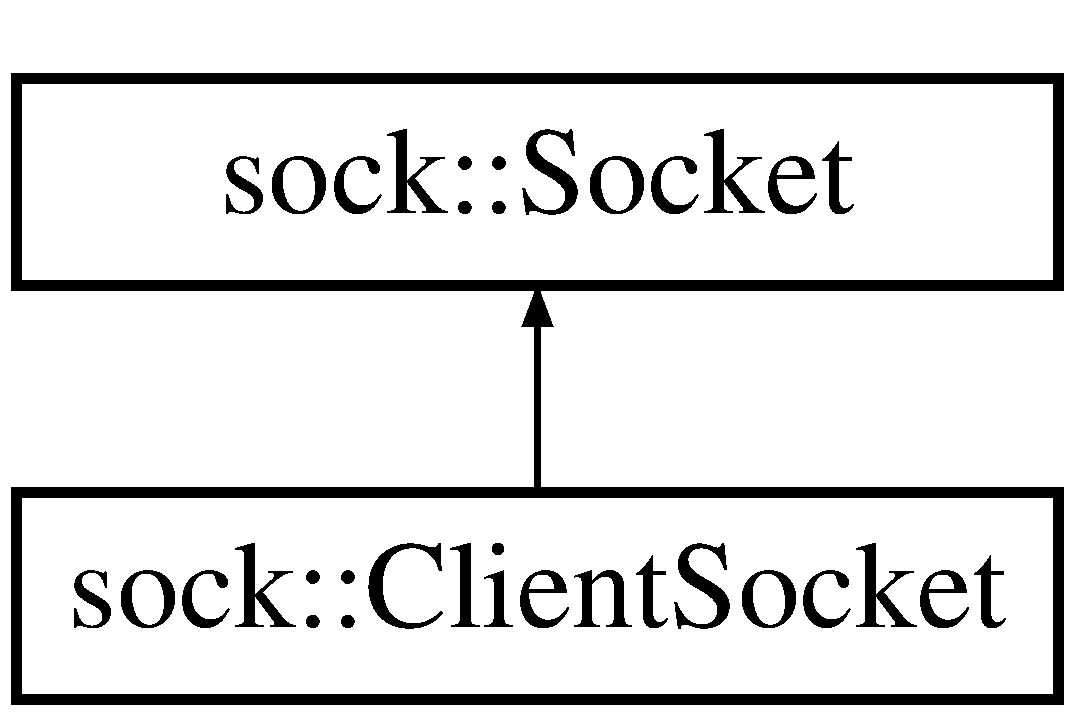
\includegraphics[height=2.000000cm]{classsock_1_1_client_socket}
\end{center}
\end{figure}
\subsection*{Public 멤버 함수}
\begin{DoxyCompactItemize}
\item 
bool \hyperlink{classsock_1_1_client_socket_af579d535f69a899beab546f668aa95bf}{connect} (const std\+::string host, const int port)
\begin{DoxyCompactList}\small\item\em 소켓을 서버와 연결하는 메소드 \end{DoxyCompactList}\end{DoxyCompactItemize}
\subsection*{추가로 상속된 멤버들}


\subsection{상세한 설명}
클라이언트 소켓 

Socket.\+hpp 파일의 85 번째 라인에서 정의되었습니다.



\subsection{멤버 함수 문서화}
\mbox{\Hypertarget{classsock_1_1_client_socket_af579d535f69a899beab546f668aa95bf}\label{classsock_1_1_client_socket_af579d535f69a899beab546f668aa95bf}} 
\index{sock\+::\+Client\+Socket@{sock\+::\+Client\+Socket}!connect@{connect}}
\index{connect@{connect}!sock\+::\+Client\+Socket@{sock\+::\+Client\+Socket}}
\subsubsection{\texorpdfstring{connect()}{connect()}}
{\footnotesize\ttfamily bool sock\+::\+Client\+Socket\+::connect (\begin{DoxyParamCaption}\item[{const std\+::string}]{host,  }\item[{const int}]{port }\end{DoxyParamCaption})}



소켓을 서버와 연결하는 메소드 


\begin{DoxyParams}{매개변수}
{\em host} & 연결할 서버의 주소 \\
\hline
{\em port} & 사용할 포트 번호 \\
\hline
\end{DoxyParams}
\begin{DoxyReturn}{반환값}
성공 시 true 그렇지 않으면 false 
\end{DoxyReturn}


Socket.\+cpp 파일의 162 번째 라인에서 정의되었습니다.



이 클래스에 대한 문서화 페이지는 다음의 파일들로부터 생성되었습니다.\+:\begin{DoxyCompactItemize}
\item 
Network/Socket.\+hpp\item 
Network/Socket.\+cpp\end{DoxyCompactItemize}

\hypertarget{classtools_1_1_dicider}{}\section{tools\+:\+:Dicider 클래스 참조}
\label{classtools_1_1_dicider}\index{tools\+::\+Dicider@{tools\+::\+Dicider}}


초기에 입력된 문자열과 비교하여 \hyperlink{classtools_1_1_dicider_afdc1fb561a2ed8037d0fa87b69a7792d}{tools\+::\+Dicider\+::\+L\+E\+A\+S\+T\+M\+A\+T\+CH} 를 넘었을 경우 결과를 도출한다.  




{\ttfamily \#include $<$Tools.\+hpp$>$}

\subsection*{Public 멤버 함수}
\begin{DoxyCompactItemize}
\item 
\mbox{\Hypertarget{classtools_1_1_dicider_a8648682b1eba05db80a14051fc0b16c6}\label{classtools_1_1_dicider_a8648682b1eba05db80a14051fc0b16c6}} 
\hyperlink{classtools_1_1_dicider_a8648682b1eba05db80a14051fc0b16c6}{Dicider} ()
\begin{DoxyCompactList}\small\item\em \hyperlink{classtools_1_1_dicider}{Dicider} 초기화 비교할 문자열을 설정한다. \end{DoxyCompactList}\item 
bool \hyperlink{classtools_1_1_dicider_a7340ce8845ca163e4bcddd73be54a0c9}{decide} (std\+::string str)
\begin{DoxyCompactList}\small\item\em 연속으로 일정 횟수까지 같은 문자열을 입력받으면 최종 결과를 출력 \end{DoxyCompactList}\end{DoxyCompactItemize}
\subsection*{정적 Public 속성}
\begin{DoxyCompactItemize}
\item 
\mbox{\Hypertarget{classtools_1_1_dicider_afdc1fb561a2ed8037d0fa87b69a7792d}\label{classtools_1_1_dicider_afdc1fb561a2ed8037d0fa87b69a7792d}} 
static const int \hyperlink{classtools_1_1_dicider_afdc1fb561a2ed8037d0fa87b69a7792d}{L\+E\+A\+S\+T\+M\+A\+T\+CH} = 5
\begin{DoxyCompactList}\small\item\em 최소한의 일치 횟수 \end{DoxyCompactList}\end{DoxyCompactItemize}
\subsection*{Private 속성}
\begin{DoxyCompactItemize}
\item 
\mbox{\Hypertarget{classtools_1_1_dicider_ad5934d4a2abed460c22ea2b6313bdb5f}\label{classtools_1_1_dicider_ad5934d4a2abed460c22ea2b6313bdb5f}} 
std\+::string \hyperlink{classtools_1_1_dicider_ad5934d4a2abed460c22ea2b6313bdb5f}{key\+Str}
\begin{DoxyCompactList}\small\item\em 초기 문자열 \end{DoxyCompactList}\item 
\mbox{\Hypertarget{classtools_1_1_dicider_acb9cec03e38fc8609c48f1acc5fb934d}\label{classtools_1_1_dicider_acb9cec03e38fc8609c48f1acc5fb934d}} 
int \hyperlink{classtools_1_1_dicider_acb9cec03e38fc8609c48f1acc5fb934d}{match}
\begin{DoxyCompactList}\small\item\em 일치한 횟수 \end{DoxyCompactList}\end{DoxyCompactItemize}


\subsection{상세한 설명}
초기에 입력된 문자열과 비교하여 \hyperlink{classtools_1_1_dicider_afdc1fb561a2ed8037d0fa87b69a7792d}{tools\+::\+Dicider\+::\+L\+E\+A\+S\+T\+M\+A\+T\+CH} 를 넘었을 경우 결과를 도출한다. 

Tools.\+hpp 파일의 32 번째 라인에서 정의되었습니다.



\subsection{멤버 함수 문서화}
\mbox{\Hypertarget{classtools_1_1_dicider_a7340ce8845ca163e4bcddd73be54a0c9}\label{classtools_1_1_dicider_a7340ce8845ca163e4bcddd73be54a0c9}} 
\index{tools\+::\+Dicider@{tools\+::\+Dicider}!decide@{decide}}
\index{decide@{decide}!tools\+::\+Dicider@{tools\+::\+Dicider}}
\subsubsection{\texorpdfstring{decide()}{decide()}}
{\footnotesize\ttfamily bool tools\+::\+Dicider\+::decide (\begin{DoxyParamCaption}\item[{std\+::string}]{str }\end{DoxyParamCaption})}



연속으로 일정 횟수까지 같은 문자열을 입력받으면 최종 결과를 출력 


\begin{DoxyParams}{매개변수}
{\em str} & 비교 문자열 \\
\hline
\end{DoxyParams}
\begin{DoxyReturn}{반환값}
str과 초기 문자열이 L\+E\+A\+S\+T\+M\+A\+T\+CH 의 횟수 이상 일치할 경우 true 그렇지 않으면 false 을 반환 
\end{DoxyReturn}


Tools.\+cpp 파일의 19 번째 라인에서 정의되었습니다.



이 클래스에 대한 문서화 페이지는 다음의 파일들로부터 생성되었습니다.\+:\begin{DoxyCompactItemize}
\item 
Opencv/Tools.\+hpp\item 
Opencv/Tools.\+cpp\end{DoxyCompactItemize}

\hypertarget{structhttp_1_1_header_line}{}\section{http\+:\+:Header\+Line 구조체 참조}
\label{structhttp_1_1_header_line}\index{http\+::\+Header\+Line@{http\+::\+Header\+Line}}


\hyperlink{classhttp_1_1_message}{Message} 를 구성하는 헤더  




{\ttfamily \#include $<$Http.\+hpp$>$}

\subsection*{Public 속성}
\begin{DoxyCompactItemize}
\item 
\mbox{\Hypertarget{structhttp_1_1_header_line_aab3fde3ed409272848cac9eb5b210f67}\label{structhttp_1_1_header_line_aab3fde3ed409272848cac9eb5b210f67}} 
std\+::string \hyperlink{structhttp_1_1_header_line_aab3fde3ed409272848cac9eb5b210f67}{field}
\begin{DoxyCompactList}\small\item\em 필드명 \end{DoxyCompactList}\item 
\mbox{\Hypertarget{structhttp_1_1_header_line_a507bcfbe25b42ba790797d63ae45bc38}\label{structhttp_1_1_header_line_a507bcfbe25b42ba790797d63ae45bc38}} 
std\+::string \hyperlink{structhttp_1_1_header_line_a507bcfbe25b42ba790797d63ae45bc38}{value}
\begin{DoxyCompactList}\small\item\em 값 \end{DoxyCompactList}\end{DoxyCompactItemize}


\subsection{상세한 설명}
\hyperlink{classhttp_1_1_message}{Message} 를 구성하는 헤더 

Http.\+hpp 파일의 21 번째 라인에서 정의되었습니다.



이 구조체에 대한 문서화 페이지는 다음의 파일로부터 생성되었습니다.\+:\begin{DoxyCompactItemize}
\item 
Network/Http.\+hpp\end{DoxyCompactItemize}

\hypertarget{classhttp_1_1_message}{}\section{http\+:\+:Message 클래스 참조}
\label{classhttp_1_1_message}\index{http\+::\+Message@{http\+::\+Message}}


H\+T\+TP 메세지  




{\ttfamily \#include $<$Http.\+hpp$>$}

http\+:\+:Message에 대한 상속 다이어그램 \+: \begin{figure}[H]
\begin{center}
\leavevmode
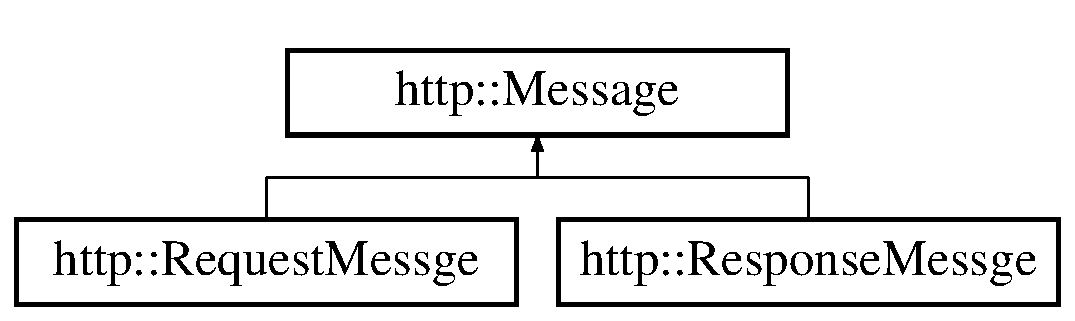
\includegraphics[height=2.000000cm]{classhttp_1_1_message}
\end{center}
\end{figure}
\subsection*{Public 멤버 함수}
\begin{DoxyCompactItemize}
\item 
\hyperlink{classhttp_1_1_message_af708fe5d0db7f88afe44665ddcf2205a}{Message} (std\+::string msg)
\begin{DoxyCompactList}\small\item\em H\+T\+TP 메세지의 문자열을 입력 받아 \hyperlink{classhttp_1_1_message}{Message} 를 만드는 생성자 \end{DoxyCompactList}\item 
\hyperlink{classhttp_1_1_message_a3b0418444366710791deda1abe0f9f9f}{Message} (std\+::string \hyperlink{classhttp_1_1_message_a56420a38395db02e6bc33bf27a6c7769}{first\+Line}\mbox{[}$\,$\mbox{]}, \hyperlink{structhttp_1_1_header_line}{Header\+Line} header\+Line\mbox{[}$\,$\mbox{]}, int \hyperlink{classhttp_1_1_message_abf4fab93257b3d37930ed20627f1c061}{header\+Size}, std\+::string content)
\begin{DoxyCompactList}\small\item\em H\+T\+TP 메세지의 첫줄과 파싱된 \hyperlink{structhttp_1_1_header_line}{Header\+Line} 과 Body를 이용하여 \hyperlink{classhttp_1_1_message}{Message} 를 만드는 생성자 \end{DoxyCompactList}\item 
\hyperlink{structhttp_1_1_header_line}{Header\+Line} \hyperlink{classhttp_1_1_message_a8f81090365d2147e31cc750498b846e7}{get\+Header} (int index)
\begin{DoxyCompactList}\small\item\em index 번째의 헤더를 불러오는 메소드 \end{DoxyCompactList}\item 
std\+::string \hyperlink{classhttp_1_1_message_a23c2c7bdf00670719c5493742f38eaa3}{get\+Message\+Body} ()
\begin{DoxyCompactList}\small\item\em H\+T\+TP 메세지의 Body를 불러 오는 메소드 \end{DoxyCompactList}\item 
int \hyperlink{classhttp_1_1_message_a5904d9972df76c1bc751d1bb352c3849}{get\+Header\+Size} ()
\begin{DoxyCompactList}\small\item\em H\+T\+TP 메세지를 구성하는 헤더들의 갯수를 불러오는 메소드 \end{DoxyCompactList}\item 
std\+::string \hyperlink{classhttp_1_1_message_a4bc25a6f276e17cd9975ecdaa0d4093a}{get\+String} ()
\begin{DoxyCompactList}\small\item\em 파싱된 문자열을 H\+T\+TP 메시지로 불러오는 메소드 \end{DoxyCompactList}\end{DoxyCompactItemize}
\subsection*{Protected 속성}
\begin{DoxyCompactItemize}
\item 
\mbox{\Hypertarget{classhttp_1_1_message_a56420a38395db02e6bc33bf27a6c7769}\label{classhttp_1_1_message_a56420a38395db02e6bc33bf27a6c7769}} 
std\+::string \hyperlink{classhttp_1_1_message_a56420a38395db02e6bc33bf27a6c7769}{first\+Line} \mbox{[}\hyperlink{classhttp_1_1_message_a0ff1ef5648a30bcb43d48550f06eb976}{F\+I\+R\+S\+T\+L\+I\+N\+E\+S\+I\+ZE}\mbox{]}
\begin{DoxyCompactList}\small\item\em 첫줄 토큰들 \end{DoxyCompactList}\end{DoxyCompactItemize}
\subsection*{정적 Protected 속성}
\begin{DoxyCompactItemize}
\item 
\mbox{\Hypertarget{classhttp_1_1_message_a0ff1ef5648a30bcb43d48550f06eb976}\label{classhttp_1_1_message_a0ff1ef5648a30bcb43d48550f06eb976}} 
static const int \hyperlink{classhttp_1_1_message_a0ff1ef5648a30bcb43d48550f06eb976}{F\+I\+R\+S\+T\+L\+I\+N\+E\+S\+I\+ZE} = 3
\begin{DoxyCompactList}\small\item\em 메세지의 첫줄의 토큰 갯수 \end{DoxyCompactList}\end{DoxyCompactItemize}
\subsection*{Private 멤버 함수}
\begin{DoxyCompactItemize}
\item 
void \hyperlink{classhttp_1_1_message_aa7346502a360e77b2da5cc9a35821a32}{parser} (std\+::string input, std\+::string key, std\+::string output\mbox{[}$\,$\mbox{]}, int size)
\begin{DoxyCompactList}\small\item\em H\+T\+TP 메세지를 크기에 맞게 파싱하는 메소드 \end{DoxyCompactList}\end{DoxyCompactItemize}
\subsection*{Private 속성}
\begin{DoxyCompactItemize}
\item 
\mbox{\Hypertarget{classhttp_1_1_message_a4a238c04c3a7b2e49c640eb0784f3798}\label{classhttp_1_1_message_a4a238c04c3a7b2e49c640eb0784f3798}} 
\hyperlink{structhttp_1_1_header_line}{Header\+Line} $\ast$ \hyperlink{classhttp_1_1_message_a4a238c04c3a7b2e49c640eb0784f3798}{header}
\begin{DoxyCompactList}\small\item\em 헤더 \end{DoxyCompactList}\item 
\mbox{\Hypertarget{classhttp_1_1_message_afcad3d09b8389e5e7c0d6eb433b69be4}\label{classhttp_1_1_message_afcad3d09b8389e5e7c0d6eb433b69be4}} 
std\+::string \hyperlink{classhttp_1_1_message_afcad3d09b8389e5e7c0d6eb433b69be4}{message\+Body}
\begin{DoxyCompactList}\small\item\em 메세지의 Body \end{DoxyCompactList}\item 
\mbox{\Hypertarget{classhttp_1_1_message_abf4fab93257b3d37930ed20627f1c061}\label{classhttp_1_1_message_abf4fab93257b3d37930ed20627f1c061}} 
int \hyperlink{classhttp_1_1_message_abf4fab93257b3d37930ed20627f1c061}{header\+Size}
\begin{DoxyCompactList}\small\item\em 헤더의 갯수 \end{DoxyCompactList}\end{DoxyCompactItemize}
\subsection*{정적 Private 속성}
\begin{DoxyCompactItemize}
\item 
\mbox{\Hypertarget{classhttp_1_1_message_abc49c33614b0bb3cab83f764cad9d1c1}\label{classhttp_1_1_message_abc49c33614b0bb3cab83f764cad9d1c1}} 
static const int \hyperlink{classhttp_1_1_message_abc49c33614b0bb3cab83f764cad9d1c1}{M\+A\+X\+H\+E\+A\+D\+E\+RS} = 100
\begin{DoxyCompactList}\small\item\em 헤더의 최대 갯수 \end{DoxyCompactList}\end{DoxyCompactItemize}


\subsection{상세한 설명}
H\+T\+TP 메세지 

Http.\+hpp 파일의 47 번째 라인에서 정의되었습니다.



\subsection{생성자 \& 소멸자 문서화}
\mbox{\Hypertarget{classhttp_1_1_message_af708fe5d0db7f88afe44665ddcf2205a}\label{classhttp_1_1_message_af708fe5d0db7f88afe44665ddcf2205a}} 
\index{http\+::\+Message@{http\+::\+Message}!Message@{Message}}
\index{Message@{Message}!http\+::\+Message@{http\+::\+Message}}
\subsubsection{\texorpdfstring{Message()}{Message()}\hspace{0.1cm}{\footnotesize\ttfamily [1/2]}}
{\footnotesize\ttfamily http\+::\+Message\+::\+Message (\begin{DoxyParamCaption}\item[{std\+::string}]{msg }\end{DoxyParamCaption})}



H\+T\+TP 메세지의 문자열을 입력 받아 \hyperlink{classhttp_1_1_message}{Message} 를 만드는 생성자 

이 함수는 편의를 제공하기 위해 오버로드된 멤버 함수입니다. 위의 함수와 틀린 점은 단지 받아들이는 아규먼트(argument)가 다르다는 것입니다. 
\begin{DoxyParams}{매개변수}
{\em msg} & H\+T\+TP 메세지의 문자열 \\
\hline
\end{DoxyParams}


Http.\+cpp 파일의 28 번째 라인에서 정의되었습니다.

\mbox{\Hypertarget{classhttp_1_1_message_a3b0418444366710791deda1abe0f9f9f}\label{classhttp_1_1_message_a3b0418444366710791deda1abe0f9f9f}} 
\index{http\+::\+Message@{http\+::\+Message}!Message@{Message}}
\index{Message@{Message}!http\+::\+Message@{http\+::\+Message}}
\subsubsection{\texorpdfstring{Message()}{Message()}\hspace{0.1cm}{\footnotesize\ttfamily [2/2]}}
{\footnotesize\ttfamily http\+::\+Message\+::\+Message (\begin{DoxyParamCaption}\item[{std\+::string}]{first\+Line\mbox{[}$\,$\mbox{]},  }\item[{\hyperlink{structhttp_1_1_header_line}{Header\+Line}}]{header\+Line\mbox{[}$\,$\mbox{]},  }\item[{int}]{header\+Size,  }\item[{std\+::string}]{content }\end{DoxyParamCaption})}



H\+T\+TP 메세지의 첫줄과 파싱된 \hyperlink{structhttp_1_1_header_line}{Header\+Line} 과 Body를 이용하여 \hyperlink{classhttp_1_1_message}{Message} 를 만드는 생성자 

이 함수는 편의를 제공하기 위해 오버로드된 멤버 함수입니다. 위의 함수와 틀린 점은 단지 받아들이는 아규먼트(argument)가 다르다는 것입니다. 
\begin{DoxyParams}{매개변수}
{\em first\+Line} & H\+T\+TP 메세지의 첫번째 줄 ( 상태 라인이나 요청 라인을 나타냄 ) \\
\hline
{\em header\+Line} & H\+T\+TP 메세지의 헤더 라인들 \\
\hline
{\em header\+Size} & 헤더 라인의 갯수 \\
\hline
{\em content} & H\+T\+TP 메세지의 Body \\
\hline
\end{DoxyParams}


Http.\+cpp 파일의 13 번째 라인에서 정의되었습니다.



\subsection{멤버 함수 문서화}
\mbox{\Hypertarget{classhttp_1_1_message_a8f81090365d2147e31cc750498b846e7}\label{classhttp_1_1_message_a8f81090365d2147e31cc750498b846e7}} 
\index{http\+::\+Message@{http\+::\+Message}!get\+Header@{get\+Header}}
\index{get\+Header@{get\+Header}!http\+::\+Message@{http\+::\+Message}}
\subsubsection{\texorpdfstring{get\+Header()}{getHeader()}}
{\footnotesize\ttfamily \hyperlink{structhttp_1_1_header_line}{http\+::\+Header\+Line} http\+::\+Message\+::get\+Header (\begin{DoxyParamCaption}\item[{int}]{index }\end{DoxyParamCaption})}



index 번째의 헤더를 불러오는 메소드 


\begin{DoxyParams}{매개변수}
{\em index} & 불러올 헤더의 인덱스 번호 \\
\hline
\end{DoxyParams}
\begin{DoxyReturn}{반환값}
index 번째의 헤더 
\end{DoxyReturn}


Http.\+cpp 파일의 76 번째 라인에서 정의되었습니다.

\mbox{\Hypertarget{classhttp_1_1_message_a5904d9972df76c1bc751d1bb352c3849}\label{classhttp_1_1_message_a5904d9972df76c1bc751d1bb352c3849}} 
\index{http\+::\+Message@{http\+::\+Message}!get\+Header\+Size@{get\+Header\+Size}}
\index{get\+Header\+Size@{get\+Header\+Size}!http\+::\+Message@{http\+::\+Message}}
\subsubsection{\texorpdfstring{get\+Header\+Size()}{getHeaderSize()}}
{\footnotesize\ttfamily int http\+::\+Message\+::get\+Header\+Size (\begin{DoxyParamCaption}{ }\end{DoxyParamCaption})}



H\+T\+TP 메세지를 구성하는 헤더들의 갯수를 불러오는 메소드 

\begin{DoxyReturn}{반환값}
헤더들의 갯수 
\end{DoxyReturn}


Http.\+cpp 파일의 88 번째 라인에서 정의되었습니다.

\mbox{\Hypertarget{classhttp_1_1_message_a23c2c7bdf00670719c5493742f38eaa3}\label{classhttp_1_1_message_a23c2c7bdf00670719c5493742f38eaa3}} 
\index{http\+::\+Message@{http\+::\+Message}!get\+Message\+Body@{get\+Message\+Body}}
\index{get\+Message\+Body@{get\+Message\+Body}!http\+::\+Message@{http\+::\+Message}}
\subsubsection{\texorpdfstring{get\+Message\+Body()}{getMessageBody()}}
{\footnotesize\ttfamily std\+::string http\+::\+Message\+::get\+Message\+Body (\begin{DoxyParamCaption}{ }\end{DoxyParamCaption})}



H\+T\+TP 메세지의 Body를 불러 오는 메소드 

\begin{DoxyReturn}{반환값}
H\+T\+TP 메세지의 Body 
\end{DoxyReturn}


Http.\+cpp 파일의 82 번째 라인에서 정의되었습니다.

\mbox{\Hypertarget{classhttp_1_1_message_a4bc25a6f276e17cd9975ecdaa0d4093a}\label{classhttp_1_1_message_a4bc25a6f276e17cd9975ecdaa0d4093a}} 
\index{http\+::\+Message@{http\+::\+Message}!get\+String@{get\+String}}
\index{get\+String@{get\+String}!http\+::\+Message@{http\+::\+Message}}
\subsubsection{\texorpdfstring{get\+String()}{getString()}}
{\footnotesize\ttfamily std\+::string http\+::\+Message\+::get\+String (\begin{DoxyParamCaption}{ }\end{DoxyParamCaption})}



파싱된 문자열을 H\+T\+TP 메시지로 불러오는 메소드 

\begin{DoxyReturn}{반환값}
문자열로 이루어진 H\+T\+TP 메세지 
\end{DoxyReturn}


Http.\+cpp 파일의 114 번째 라인에서 정의되었습니다.

\mbox{\Hypertarget{classhttp_1_1_message_aa7346502a360e77b2da5cc9a35821a32}\label{classhttp_1_1_message_aa7346502a360e77b2da5cc9a35821a32}} 
\index{http\+::\+Message@{http\+::\+Message}!parser@{parser}}
\index{parser@{parser}!http\+::\+Message@{http\+::\+Message}}
\subsubsection{\texorpdfstring{parser()}{parser()}}
{\footnotesize\ttfamily void http\+::\+Message\+::parser (\begin{DoxyParamCaption}\item[{std\+::string}]{input,  }\item[{std\+::string}]{key,  }\item[{std\+::string}]{output\mbox{[}$\,$\mbox{]},  }\item[{int}]{size }\end{DoxyParamCaption})\hspace{0.3cm}{\ttfamily [private]}}



H\+T\+TP 메세지를 크기에 맞게 파싱하는 메소드 


\begin{DoxyParams}{매개변수}
{\em input} & 파싱할 문자열 \\
\hline
{\em key} & 각 토큰을 구분할 키 문자열 \\
\hline
{\em output} & 파싱된 결과 생성된 토큰 \\
\hline
{\em size} & 출력되는 토큰의 크기 \\
\hline
\end{DoxyParams}


Http.\+cpp 파일의 94 번째 라인에서 정의되었습니다.



이 클래스에 대한 문서화 페이지는 다음의 파일들로부터 생성되었습니다.\+:\begin{DoxyCompactItemize}
\item 
Network/Http.\+hpp\item 
Network/Http.\+cpp\end{DoxyCompactItemize}

\hypertarget{class_o_c_r}{}\section{O\+CR 클래스 참조}
\label{class_o_c_r}\index{O\+CR@{O\+CR}}


Artificial Neural Networks을 다루기 위한 클래스  




{\ttfamily \#include $<$O\+C\+R.\+hpp$>$}

\subsection*{Public 타입}
\begin{DoxyCompactItemize}
\item 
enum \hyperlink{class_o_c_r_a442cab5841719df30befa282835b4eb3}{M\+O\+DE} \{ \hyperlink{class_o_c_r_a442cab5841719df30befa282835b4eb3a85eb8164b9c5fc654a6492994fe80289}{R\+E\+A\+D\+DT} = 0b00, 
\hyperlink{class_o_c_r_a442cab5841719df30befa282835b4eb3a885a5ee83c76766fe4189e8e90247797}{C\+O\+L\+L\+E\+CT} = 0b01, 
\hyperlink{class_o_c_r_a442cab5841719df30befa282835b4eb3a3439e4119033288be0dd0a3a00a2d6fd}{W\+R\+I\+T\+E\+DT} = 0b11
 \}\begin{DoxyCompactList}\small\item\em 훈련 데이터를 다룰 방법 \end{DoxyCompactList}
\end{DoxyCompactItemize}
\subsection*{Public 멤버 함수}
\begin{DoxyCompactItemize}
\item 
\hyperlink{class_o_c_r_a58dd005225af496e3ccdd69f387b5865}{O\+CR} (const F\+O\+R\+M\+AT format, const int mode)
\begin{DoxyCompactList}\small\item\em \hyperlink{class_o_c_r}{O\+CR} 초기화 \end{DoxyCompactList}\item 
float \hyperlink{class_o_c_r_aee086012d86e877ac029cdde3927a221}{predict} (const cv\+::\+Mat \&img, cv\+::\+Mat $\ast$out)
\begin{DoxyCompactList}\small\item\em 입력된 Sample이 훈련된 Artificial Neural Networks의해 예측된 결과를 출력 \end{DoxyCompactList}\item 
char \hyperlink{class_o_c_r_a3d521746f28d2843381c7d7e5eedddcd}{classify} (cv\+::\+Mat $\ast$output)
\begin{DoxyCompactList}\small\item\em 예측된 결과 중 가장 가능성이 높은 문자를 추출 \end{DoxyCompactList}\end{DoxyCompactItemize}
\subsection*{정적 Public 멤버 함수}
\begin{DoxyCompactItemize}
\item 
static cv\+::\+Mat \hyperlink{class_o_c_r_ada88a7c2579124895eb6f19383749e9c}{features} (const cv\+::\+Mat \&texts, const int size\+Data)
\begin{DoxyCompactList}\small\item\em features 추출 \end{DoxyCompactList}\end{DoxyCompactItemize}
\subsection*{Public 속성}
\begin{DoxyCompactItemize}
\item 
\mbox{\Hypertarget{class_o_c_r_a9e52aa42898bfdaeef338e1ac6507233}\label{class_o_c_r_a9e52aa42898bfdaeef338e1ac6507233}} 
int \hyperlink{class_o_c_r_a9e52aa42898bfdaeef338e1ac6507233}{num\+Characters}
\begin{DoxyCompactList}\small\item\em 출력될 vector의 크기 \end{DoxyCompactList}\end{DoxyCompactItemize}
\subsection*{Private 타입}
\begin{DoxyCompactItemize}
\item 
enum \hyperlink{class_o_c_r_ad50a9d013dc2ee50341eee5b9e326686}{O\+R\+I\+E\+N\+T\+A\+T\+I\+ON} \{ \hyperlink{class_o_c_r_ad50a9d013dc2ee50341eee5b9e326686a6df62411d3b46574d518ec4d6be10a89}{V\+E\+R\+T\+I\+C\+AL} = 0, 
\hyperlink{class_o_c_r_ad50a9d013dc2ee50341eee5b9e326686a9561e34d3db489309a61726ba3e523fe}{H\+O\+R\+I\+Z\+O\+N\+T\+AL} = 1
 \}\begin{DoxyCompactList}\small\item\em Histogram 추출 시의 방향 \end{DoxyCompactList}
\end{DoxyCompactItemize}
\subsection*{Private 멤버 함수}
\begin{DoxyCompactItemize}
\item 
\mbox{\Hypertarget{class_o_c_r_a9d4b78ff145b1e89ac05eb0f194d1948}\label{class_o_c_r_a9d4b78ff145b1e89ac05eb0f194d1948}} 
void \hyperlink{class_o_c_r_a9d4b78ff145b1e89ac05eb0f194d1948}{collect\+Train\+Images} ()
\begin{DoxyCompactList}\small\item\em Train\+Number에서 훈련 데이터 불러오기 \textquotesingle{}Train\+Number\textquotesingle{}에 경로에서 모든 이미지 파일을 읽어들여 훈련 데이터를 생성한다. \end{DoxyCompactList}\item 
void \hyperlink{class_o_c_r_aac52dda47989cde2ba9c674de77bd2ce}{write\+Traindata} (const std\+::string fn)
\begin{DoxyCompactList}\small\item\em 훈련 데이터를 File System에 Json 파일로 쓰기 \end{DoxyCompactList}\item 
void \hyperlink{class_o_c_r_a27494f2dca260d6710c332897c31f716}{read\+Traindata} (const std\+::string fn)
\begin{DoxyCompactList}\small\item\em 훈련 데이터를 File System에서 Json 파일로부터 불러오기 \end{DoxyCompactList}\item 
void \hyperlink{class_o_c_r_acef1528ddf01f01f301dcd489ec427fb}{read\+Traindata} (const std\+::string fn, const F\+O\+R\+M\+AT format)
\begin{DoxyCompactList}\small\item\em 훈련 데이터를 File System에서 Json 파일로부터 불러오기 \end{DoxyCompactList}\end{DoxyCompactItemize}
\subsection*{정적 Private 멤버 함수}
\begin{DoxyCompactItemize}
\item 
static cv\+::\+Mat \hyperlink{class_o_c_r_af4dd76ed4fdaeb65ca3768755d7e3033}{get\+Histogram} (const cv\+::\+Mat \&img, const \hyperlink{class_o_c_r_ad50a9d013dc2ee50341eee5b9e326686}{O\+R\+I\+E\+N\+T\+A\+T\+I\+ON} t)
\begin{DoxyCompactList}\small\item\em Histogram 추출 \end{DoxyCompactList}\end{DoxyCompactItemize}
\subsection*{Private 속성}
\begin{DoxyCompactItemize}
\item 
\mbox{\Hypertarget{class_o_c_r_a498a8acb578f60aad04d90704b2365b8}\label{class_o_c_r_a498a8acb578f60aad04d90704b2365b8}} 
cv\+::\+Ptr$<$ cv\+::ml\+::\+A\+N\+N\+\_\+\+M\+LP $>$ \hyperlink{class_o_c_r_a498a8acb578f60aad04d90704b2365b8}{ann}
\begin{DoxyCompactList}\small\item\em Artificial Neural Networks \end{DoxyCompactList}\item 
\mbox{\Hypertarget{class_o_c_r_a57d7a81d01e81fa3008acc53074ce73f}\label{class_o_c_r_a57d7a81d01e81fa3008acc53074ce73f}} 
cv\+::\+Mat \hyperlink{class_o_c_r_a57d7a81d01e81fa3008acc53074ce73f}{classes}
\begin{DoxyCompactList}\small\item\em training\+Data와 연관된 출력될 vector들 \end{DoxyCompactList}\item 
\mbox{\Hypertarget{class_o_c_r_a2c5101fa102a3fbb66144b3f511b3bd5}\label{class_o_c_r_a2c5101fa102a3fbb66144b3f511b3bd5}} 
cv\+::\+Mat \hyperlink{class_o_c_r_a2c5101fa102a3fbb66144b3f511b3bd5}{training\+Data}
\begin{DoxyCompactList}\small\item\em 훈련을 위한 Sample들 \end{DoxyCompactList}\item 
\mbox{\Hypertarget{class_o_c_r_acc9af89294d62414e9e7ccddd2d169dc}\label{class_o_c_r_acc9af89294d62414e9e7ccddd2d169dc}} 
std\+::string \hyperlink{class_o_c_r_acc9af89294d62414e9e7ccddd2d169dc}{str\+Characters} = \char`\"{}0123456789\+B\+C\+D\+E\+F\+G\+N\+S\+T\+V\+W\+X\+Y\char`\"{}
\begin{DoxyCompactList}\small\item\em classes와 대응되는 문자열 \end{DoxyCompactList}\end{DoxyCompactItemize}


\subsection{상세한 설명}
Artificial Neural Networks을 다루기 위한 클래스 

O\+C\+R.\+hpp 파일의 20 번째 라인에서 정의되었습니다.



\subsection{멤버 열거형 문서화}
\mbox{\Hypertarget{class_o_c_r_a442cab5841719df30befa282835b4eb3}\label{class_o_c_r_a442cab5841719df30befa282835b4eb3}} 
\index{O\+CR@{O\+CR}!M\+O\+DE@{M\+O\+DE}}
\index{M\+O\+DE@{M\+O\+DE}!O\+CR@{O\+CR}}
\subsubsection{\texorpdfstring{M\+O\+DE}{MODE}}
{\footnotesize\ttfamily enum \hyperlink{class_o_c_r_a442cab5841719df30befa282835b4eb3}{O\+C\+R\+::\+M\+O\+DE}}



훈련 데이터를 다룰 방법 

\begin{DoxyEnumFields}{열거형 멤버}
\raisebox{\heightof{T}}[0pt][0pt]{\index{R\+E\+A\+D\+DT@{R\+E\+A\+D\+DT}!O\+CR@{O\+CR}}\index{O\+CR@{O\+CR}!R\+E\+A\+D\+DT@{R\+E\+A\+D\+DT}}}\mbox{\Hypertarget{class_o_c_r_a442cab5841719df30befa282835b4eb3a85eb8164b9c5fc654a6492994fe80289}\label{class_o_c_r_a442cab5841719df30befa282835b4eb3a85eb8164b9c5fc654a6492994fe80289}} 
R\+E\+A\+D\+DT&Json File에서 읽기 \begin{DoxySeeAlso}{참고}
\hyperlink{class_o_c_r_a27494f2dca260d6710c332897c31f716}{read\+Traindata} 
\end{DoxySeeAlso}
\\
\hline

\raisebox{\heightof{T}}[0pt][0pt]{\index{C\+O\+L\+L\+E\+CT@{C\+O\+L\+L\+E\+CT}!O\+CR@{O\+CR}}\index{O\+CR@{O\+CR}!C\+O\+L\+L\+E\+CT@{C\+O\+L\+L\+E\+CT}}}\mbox{\Hypertarget{class_o_c_r_a442cab5841719df30befa282835b4eb3a885a5ee83c76766fe4189e8e90247797}\label{class_o_c_r_a442cab5841719df30befa282835b4eb3a885a5ee83c76766fe4189e8e90247797}} 
C\+O\+L\+L\+E\+CT&Train\+Image에서 읽기 \begin{DoxySeeAlso}{참고}
\hyperlink{class_o_c_r_a9d4b78ff145b1e89ac05eb0f194d1948}{collect\+Train\+Images} 
\end{DoxySeeAlso}
\\
\hline

\raisebox{\heightof{T}}[0pt][0pt]{\index{W\+R\+I\+T\+E\+DT@{W\+R\+I\+T\+E\+DT}!O\+CR@{O\+CR}}\index{O\+CR@{O\+CR}!W\+R\+I\+T\+E\+DT@{W\+R\+I\+T\+E\+DT}}}\mbox{\Hypertarget{class_o_c_r_a442cab5841719df30befa282835b4eb3a3439e4119033288be0dd0a3a00a2d6fd}\label{class_o_c_r_a442cab5841719df30befa282835b4eb3a3439e4119033288be0dd0a3a00a2d6fd}} 
W\+R\+I\+T\+E\+DT&Json File로 쓰기 \begin{DoxySeeAlso}{참고}
\hyperlink{class_o_c_r_aac52dda47989cde2ba9c674de77bd2ce}{write\+Traindata} 
\end{DoxySeeAlso}
\\
\hline

\end{DoxyEnumFields}


O\+C\+R.\+hpp 파일의 72 번째 라인에서 정의되었습니다.

\mbox{\Hypertarget{class_o_c_r_ad50a9d013dc2ee50341eee5b9e326686}\label{class_o_c_r_ad50a9d013dc2ee50341eee5b9e326686}} 
\index{O\+CR@{O\+CR}!O\+R\+I\+E\+N\+T\+A\+T\+I\+ON@{O\+R\+I\+E\+N\+T\+A\+T\+I\+ON}}
\index{O\+R\+I\+E\+N\+T\+A\+T\+I\+ON@{O\+R\+I\+E\+N\+T\+A\+T\+I\+ON}!O\+CR@{O\+CR}}
\subsubsection{\texorpdfstring{O\+R\+I\+E\+N\+T\+A\+T\+I\+ON}{ORIENTATION}}
{\footnotesize\ttfamily enum \hyperlink{class_o_c_r_ad50a9d013dc2ee50341eee5b9e326686}{O\+C\+R\+::\+O\+R\+I\+E\+N\+T\+A\+T\+I\+ON}\hspace{0.3cm}{\ttfamily [private]}}



Histogram 추출 시의 방향 

\begin{DoxyEnumFields}{열거형 멤버}
\raisebox{\heightof{T}}[0pt][0pt]{\index{V\+E\+R\+T\+I\+C\+AL@{V\+E\+R\+T\+I\+C\+AL}!O\+CR@{O\+CR}}\index{O\+CR@{O\+CR}!V\+E\+R\+T\+I\+C\+AL@{V\+E\+R\+T\+I\+C\+AL}}}\mbox{\Hypertarget{class_o_c_r_ad50a9d013dc2ee50341eee5b9e326686a6df62411d3b46574d518ec4d6be10a89}\label{class_o_c_r_ad50a9d013dc2ee50341eee5b9e326686a6df62411d3b46574d518ec4d6be10a89}} 
V\+E\+R\+T\+I\+C\+AL&수직 \\
\hline

\raisebox{\heightof{T}}[0pt][0pt]{\index{H\+O\+R\+I\+Z\+O\+N\+T\+AL@{H\+O\+R\+I\+Z\+O\+N\+T\+AL}!O\+CR@{O\+CR}}\index{O\+CR@{O\+CR}!H\+O\+R\+I\+Z\+O\+N\+T\+AL@{H\+O\+R\+I\+Z\+O\+N\+T\+AL}}}\mbox{\Hypertarget{class_o_c_r_ad50a9d013dc2ee50341eee5b9e326686a9561e34d3db489309a61726ba3e523fe}\label{class_o_c_r_ad50a9d013dc2ee50341eee5b9e326686a9561e34d3db489309a61726ba3e523fe}} 
H\+O\+R\+I\+Z\+O\+N\+T\+AL&수평 \\
\hline

\end{DoxyEnumFields}


O\+C\+R.\+hpp 파일의 24 번째 라인에서 정의되었습니다.



\subsection{생성자 \& 소멸자 문서화}
\mbox{\Hypertarget{class_o_c_r_a58dd005225af496e3ccdd69f387b5865}\label{class_o_c_r_a58dd005225af496e3ccdd69f387b5865}} 
\index{O\+CR@{O\+CR}!O\+CR@{O\+CR}}
\index{O\+CR@{O\+CR}!O\+CR@{O\+CR}}
\subsubsection{\texorpdfstring{O\+C\+R()}{OCR()}}
{\footnotesize\ttfamily O\+C\+R\+::\+O\+CR (\begin{DoxyParamCaption}\item[{const F\+O\+R\+M\+AT}]{format,  }\item[{const int}]{mode }\end{DoxyParamCaption})}



\hyperlink{class_o_c_r}{O\+CR} 초기화 


\begin{DoxyParams}{매개변수}
{\em format} & O\+C\+R이 인식할 형식 \\
\hline
{\em mode} & 훈련 데이터를 다룰 방법 \\
\hline
\end{DoxyParams}


O\+C\+R.\+cpp 파일의 7 번째 라인에서 정의되었습니다.



\subsection{멤버 함수 문서화}
\mbox{\Hypertarget{class_o_c_r_a3d521746f28d2843381c7d7e5eedddcd}\label{class_o_c_r_a3d521746f28d2843381c7d7e5eedddcd}} 
\index{O\+CR@{O\+CR}!classify@{classify}}
\index{classify@{classify}!O\+CR@{O\+CR}}
\subsubsection{\texorpdfstring{classify()}{classify()}}
{\footnotesize\ttfamily char O\+C\+R\+::classify (\begin{DoxyParamCaption}\item[{cv\+::\+Mat $\ast$}]{output }\end{DoxyParamCaption})}



예측된 결과 중 가장 가능성이 높은 문자를 추출 


\begin{DoxyParams}{매개변수}
{\em output} & 문자를 추출할 결과 매트릭스 \\
\hline
\end{DoxyParams}
\begin{DoxyReturn}{반환값}
가능성 높은 문자 
\end{DoxyReturn}


O\+C\+R.\+cpp 파일의 136 번째 라인에서 정의되었습니다.

\mbox{\Hypertarget{class_o_c_r_ada88a7c2579124895eb6f19383749e9c}\label{class_o_c_r_ada88a7c2579124895eb6f19383749e9c}} 
\index{O\+CR@{O\+CR}!features@{features}}
\index{features@{features}!O\+CR@{O\+CR}}
\subsubsection{\texorpdfstring{features()}{features()}}
{\footnotesize\ttfamily Mat O\+C\+R\+::features (\begin{DoxyParamCaption}\item[{const cv\+::\+Mat \&}]{texts,  }\item[{const int}]{size\+Data }\end{DoxyParamCaption})\hspace{0.3cm}{\ttfamily [static]}}



features 추출 


\begin{DoxyParams}{매개변수}
{\em texts} & features을 추출할 이미지 \\
\hline
{\em size\+Data} & 추출될 features의 가로 세로 크기 \\
\hline
\end{DoxyParams}
\begin{DoxyReturn}{반환값}
입력받은 이미지에 대한 features 
\end{DoxyReturn}


O\+C\+R.\+cpp 파일의 171 번째 라인에서 정의되었습니다.

\mbox{\Hypertarget{class_o_c_r_af4dd76ed4fdaeb65ca3768755d7e3033}\label{class_o_c_r_af4dd76ed4fdaeb65ca3768755d7e3033}} 
\index{O\+CR@{O\+CR}!get\+Histogram@{get\+Histogram}}
\index{get\+Histogram@{get\+Histogram}!O\+CR@{O\+CR}}
\subsubsection{\texorpdfstring{get\+Histogram()}{getHistogram()}}
{\footnotesize\ttfamily Mat O\+C\+R\+::get\+Histogram (\begin{DoxyParamCaption}\item[{const cv\+::\+Mat \&}]{img,  }\item[{const \hyperlink{class_o_c_r_ad50a9d013dc2ee50341eee5b9e326686}{O\+R\+I\+E\+N\+T\+A\+T\+I\+ON}}]{t }\end{DoxyParamCaption})\hspace{0.3cm}{\ttfamily [static]}, {\ttfamily [private]}}



Histogram 추출 


\begin{DoxyParams}{매개변수}
{\em img} & Histogram을 추출할 이미지 \\
\hline
{\em t} & Histogram 추출 시의 방향 \\
\hline
\end{DoxyParams}
\begin{DoxyReturn}{반환값}
추출된 Histogram의 매트릭스 
\end{DoxyReturn}


O\+C\+R.\+cpp 파일의 152 번째 라인에서 정의되었습니다.

\mbox{\Hypertarget{class_o_c_r_aee086012d86e877ac029cdde3927a221}\label{class_o_c_r_aee086012d86e877ac029cdde3927a221}} 
\index{O\+CR@{O\+CR}!predict@{predict}}
\index{predict@{predict}!O\+CR@{O\+CR}}
\subsubsection{\texorpdfstring{predict()}{predict()}}
{\footnotesize\ttfamily float O\+C\+R\+::predict (\begin{DoxyParamCaption}\item[{const cv\+::\+Mat \&}]{img,  }\item[{cv\+::\+Mat $\ast$}]{out }\end{DoxyParamCaption})}



입력된 Sample이 훈련된 Artificial Neural Networks의해 예측된 결과를 출력 


\begin{DoxyParams}{매개변수}
{\em img} & 입력할 Sample \\
\hline
{\em out} & 예측된 결과의 매트릭스 \\
\hline
\end{DoxyParams}
\begin{DoxyReturn}{반환값}
O\+C\+R을 통해 예측된 결과 
\end{DoxyReturn}


O\+C\+R.\+cpp 파일의 148 번째 라인에서 정의되었습니다.

\mbox{\Hypertarget{class_o_c_r_a27494f2dca260d6710c332897c31f716}\label{class_o_c_r_a27494f2dca260d6710c332897c31f716}} 
\index{O\+CR@{O\+CR}!read\+Traindata@{read\+Traindata}}
\index{read\+Traindata@{read\+Traindata}!O\+CR@{O\+CR}}
\subsubsection{\texorpdfstring{read\+Traindata()}{readTraindata()}\hspace{0.1cm}{\footnotesize\ttfamily [1/2]}}
{\footnotesize\ttfamily void O\+C\+R\+::read\+Traindata (\begin{DoxyParamCaption}\item[{const std\+::string}]{fn }\end{DoxyParamCaption})\hspace{0.3cm}{\ttfamily [private]}}



훈련 데이터를 File System에서 Json 파일로부터 불러오기 

이 함수는 편의를 제공하기 위해 오버로드된 멤버 함수입니다. 위의 함수와 틀린 점은 단지 받아들이는 아규먼트(argument)가 다르다는 것입니다. 
\begin{DoxyParams}{매개변수}
{\em fn} & Josn 파일의 경로 \\
\hline
\end{DoxyParams}


O\+C\+R.\+cpp 파일의 55 번째 라인에서 정의되었습니다.

\mbox{\Hypertarget{class_o_c_r_acef1528ddf01f01f301dcd489ec427fb}\label{class_o_c_r_acef1528ddf01f01f301dcd489ec427fb}} 
\index{O\+CR@{O\+CR}!read\+Traindata@{read\+Traindata}}
\index{read\+Traindata@{read\+Traindata}!O\+CR@{O\+CR}}
\subsubsection{\texorpdfstring{read\+Traindata()}{readTraindata()}\hspace{0.1cm}{\footnotesize\ttfamily [2/2]}}
{\footnotesize\ttfamily void O\+C\+R\+::read\+Traindata (\begin{DoxyParamCaption}\item[{const std\+::string}]{fn,  }\item[{const F\+O\+R\+M\+AT}]{format }\end{DoxyParamCaption})\hspace{0.3cm}{\ttfamily [private]}}



훈련 데이터를 File System에서 Json 파일로부터 불러오기 

이 함수는 편의를 제공하기 위해 오버로드된 멤버 함수입니다. 위의 함수와 틀린 점은 단지 받아들이는 아규먼트(argument)가 다르다는 것입니다. 
\begin{DoxyParams}{매개변수}
{\em fn} & Josn 파일의 경로 \\
\hline
{\em format} & Json O\+C\+R이 인식할 형식 \\
\hline
\end{DoxyParams}


O\+C\+R.\+cpp 파일의 69 번째 라인에서 정의되었습니다.

\mbox{\Hypertarget{class_o_c_r_aac52dda47989cde2ba9c674de77bd2ce}\label{class_o_c_r_aac52dda47989cde2ba9c674de77bd2ce}} 
\index{O\+CR@{O\+CR}!write\+Traindata@{write\+Traindata}}
\index{write\+Traindata@{write\+Traindata}!O\+CR@{O\+CR}}
\subsubsection{\texorpdfstring{write\+Traindata()}{writeTraindata()}}
{\footnotesize\ttfamily void O\+C\+R\+::write\+Traindata (\begin{DoxyParamCaption}\item[{const std\+::string}]{fn }\end{DoxyParamCaption})\hspace{0.3cm}{\ttfamily [private]}}



훈련 데이터를 File System에 Json 파일로 쓰기 


\begin{DoxyParams}{매개변수}
{\em fn} & josn 파일의 경로 \\
\hline
\end{DoxyParams}


O\+C\+R.\+cpp 파일의 100 번째 라인에서 정의되었습니다.



이 클래스에 대한 문서화 페이지는 다음의 파일들로부터 생성되었습니다.\+:\begin{DoxyCompactItemize}
\item 
Opencv/O\+C\+R.\+hpp\item 
Opencv/O\+C\+R.\+cpp\end{DoxyCompactItemize}

\hypertarget{class_o_c_r_trainer}{}\section{O\+C\+R\+Trainer 클래스 참조}
\label{class_o_c_r_trainer}\index{O\+C\+R\+Trainer@{O\+C\+R\+Trainer}}


\hyperlink{class_o_c_r_a9d4b78ff145b1e89ac05eb0f194d1948}{O\+C\+R\+::collect\+Train\+Images} 실행 시 필요한 image를 생성하는 클래스  




{\ttfamily \#include $<$O\+C\+R.\+hpp$>$}

\subsection*{Public 멤버 함수}
\begin{DoxyCompactItemize}
\item 
\hyperlink{class_o_c_r_trainer_abd29826f033646e6937bc07af133d599}{O\+C\+R\+Trainer} (const std\+::string \hyperlink{class_o_c_r_trainer_a8581e40fcbb646332572248938094b81}{answer})
\begin{DoxyCompactList}\small\item\em \hyperlink{class_o_c_r_trainer}{O\+C\+R\+Trainer} 초기화 \end{DoxyCompactList}\item 
\mbox{\Hypertarget{class_o_c_r_trainer_a0c5b71ded13ee1ac8b135a9fd0ee140d}\label{class_o_c_r_trainer_a0c5b71ded13ee1ac8b135a9fd0ee140d}} 
void \hyperlink{class_o_c_r_trainer_a0c5b71ded13ee1ac8b135a9fd0ee140d}{train} (const std\+::vector$<$ cv\+::\+Mat $>$ \&sample)
\begin{DoxyCompactList}\small\item\em \hyperlink{class_o_c_r}{O\+CR} 클래스에서 참조할 이미지를 File System에 쓰기 입력받은 이미지를 \textquotesingle{}Train\+Image\textquotesingle{}경로에 File System로 쓴다. \end{DoxyCompactList}\end{DoxyCompactItemize}
\subsection*{Private 속성}
\begin{DoxyCompactItemize}
\item 
\mbox{\Hypertarget{class_o_c_r_trainer_a9d8b8a5e578dfbe9b71f86d80662c667}\label{class_o_c_r_trainer_a9d8b8a5e578dfbe9b71f86d80662c667}} 
int \hyperlink{class_o_c_r_trainer_a9d8b8a5e578dfbe9b71f86d80662c667}{file\+Indexs} \mbox{[}N\+U\+M\+B\+ER+C\+H\+A\+R\+A\+C\+T\+ER\mbox{]}
\begin{DoxyCompactList}\small\item\em File 검색을 위한 Index 변수 \end{DoxyCompactList}\item 
\mbox{\Hypertarget{class_o_c_r_trainer_a8581e40fcbb646332572248938094b81}\label{class_o_c_r_trainer_a8581e40fcbb646332572248938094b81}} 
std\+::string \hyperlink{class_o_c_r_trainer_a8581e40fcbb646332572248938094b81}{answer}
\begin{DoxyCompactList}\small\item\em 지도학습을 위한 정답 \end{DoxyCompactList}\end{DoxyCompactItemize}


\subsection{상세한 설명}
\hyperlink{class_o_c_r_a9d4b78ff145b1e89ac05eb0f194d1948}{O\+C\+R\+::collect\+Train\+Images} 실행 시 필요한 image를 생성하는 클래스 

O\+C\+R.\+hpp 파일의 114 번째 라인에서 정의되었습니다.



\subsection{생성자 \& 소멸자 문서화}
\mbox{\Hypertarget{class_o_c_r_trainer_abd29826f033646e6937bc07af133d599}\label{class_o_c_r_trainer_abd29826f033646e6937bc07af133d599}} 
\index{O\+C\+R\+Trainer@{O\+C\+R\+Trainer}!O\+C\+R\+Trainer@{O\+C\+R\+Trainer}}
\index{O\+C\+R\+Trainer@{O\+C\+R\+Trainer}!O\+C\+R\+Trainer@{O\+C\+R\+Trainer}}
\subsubsection{\texorpdfstring{O\+C\+R\+Trainer()}{OCRTrainer()}}
{\footnotesize\ttfamily O\+C\+R\+Trainer\+::\+O\+C\+R\+Trainer (\begin{DoxyParamCaption}\item[{const std\+::string}]{answer }\end{DoxyParamCaption})}



\hyperlink{class_o_c_r_trainer}{O\+C\+R\+Trainer} 초기화 


\begin{DoxyParams}{매개변수}
{\em answer} & 지도 학습을 위한 정답 \\
\hline
\end{DoxyParams}


O\+C\+R.\+cpp 파일의 204 번째 라인에서 정의되었습니다.



이 클래스에 대한 문서화 페이지는 다음의 파일들로부터 생성되었습니다.\+:\begin{DoxyCompactItemize}
\item 
Opencv/O\+C\+R.\+hpp\item 
Opencv/O\+C\+R.\+cpp\end{DoxyCompactItemize}

\hypertarget{structprocess_1_1_parking_info}{}\section{process\+:\+:Parking\+Info 구조체 참조}
\label{structprocess_1_1_parking_info}\index{process\+::\+Parking\+Info@{process\+::\+Parking\+Info}}


주차장 정보  




{\ttfamily \#include $<$process.\+hpp$>$}

\subsection*{Public 속성}
\begin{DoxyCompactItemize}
\item 
\mbox{\Hypertarget{structprocess_1_1_parking_info_a21cc54db5d5a701d62b544d13224bafe}\label{structprocess_1_1_parking_info_a21cc54db5d5a701d62b544d13224bafe}} 
\hyperlink{namespaceprocess_aa30669026e4cf69a2550aace23bef68e}{W\+AY} \hyperlink{structprocess_1_1_parking_info_a21cc54db5d5a701d62b544d13224bafe}{way}
\begin{DoxyCompactList}\small\item\em 주차장 출입구 방향 \end{DoxyCompactList}\item 
\mbox{\Hypertarget{structprocess_1_1_parking_info_a0f83caa9ca3bf71e33a79db65ef4bff8}\label{structprocess_1_1_parking_info_a0f83caa9ca3bf71e33a79db65ef4bff8}} 
int \hyperlink{structprocess_1_1_parking_info_a0f83caa9ca3bf71e33a79db65ef4bff8}{floor}
\begin{DoxyCompactList}\small\item\em 주차장 층 \end{DoxyCompactList}\item 
\mbox{\Hypertarget{structprocess_1_1_parking_info_a0435386b258dfafdebcf6ce33648cc8d}\label{structprocess_1_1_parking_info_a0435386b258dfafdebcf6ce33648cc8d}} 
std\+::string \hyperlink{structprocess_1_1_parking_info_a0435386b258dfafdebcf6ce33648cc8d}{zone\+Name}
\begin{DoxyCompactList}\small\item\em 주차 구역 이름 \end{DoxyCompactList}\end{DoxyCompactItemize}


\subsection{상세한 설명}
주차장 정보 

이 구조체에 대한 문서화 페이지는 다음의 파일로부터 생성되었습니다.\+:\begin{DoxyCompactItemize}
\item 
Opencv/process.\+hpp\end{DoxyCompactItemize}

\hypertarget{class_plate}{}\section{Plate 클래스 참조}
\label{class_plate}\index{Plate@{Plate}}


번호판 번호판 이미지와 상대적 위치를 포함한 클래스  




{\ttfamily \#include $<$Plate.\+hpp$>$}

\subsection*{클래스}
\begin{DoxyCompactItemize}
\item 
class \hyperlink{class_plate_1_1_text}{Text}
\begin{DoxyCompactList}\small\item\em 텍스트 번호판을 구성하는 텍스트들 중 하나 \end{DoxyCompactList}\end{DoxyCompactItemize}
\subsection*{Public 멤버 함수}
\begin{DoxyCompactItemize}
\item 
\hyperlink{class_plate_a90e24aeb2c5f3120d3958999b5c673a7}{Plate} (const cv\+::\+Mat \&\hyperlink{class_plate_a51ae6ecac15e4d8b6c8f6a1f6438e84b}{img}, const cv\+::\+Point \&\hyperlink{class_plate_a9176604a4d578e74c085c6b77cef1fef}{position})
\begin{DoxyCompactList}\small\item\em \hyperlink{class_plate}{Plate} 초기화 \end{DoxyCompactList}\item 
void \hyperlink{class_plate_a4f307c5bc7cf3c5887d704fbeed3fd8a}{set\+Debug} (bool \hyperlink{class_plate_a4a417008bf85e65e2aed473f09f96b61}{debug})
\begin{DoxyCompactList}\small\item\em debug 모드 설정 \end{DoxyCompactList}\item 
bool \hyperlink{class_plate_aa18c9cc52a8a756d019faf82cd93ce13}{find\+Texts} (const int text\+Size)
\begin{DoxyCompactList}\small\item\em Plate에서 \hyperlink{class_plate_1_1_text}{Text} 이미지 추출 \end{DoxyCompactList}\item 
cv\+::\+Mat \hyperlink{class_plate_a950683b0823941cc49dd1289ea1fa259}{canonical} ()
\begin{DoxyCompactList}\small\item\em img를 정규화한 이미지 출력 \end{DoxyCompactList}\end{DoxyCompactItemize}
\subsection*{정적 Public 멤버 함수}
\begin{DoxyCompactItemize}
\item 
static void \hyperlink{class_plate_a23487b8b0975634238eb338d994c9694}{find} (const cv\+::\+Mat \&input, std\+::vector$<$ \hyperlink{class_plate}{Plate} $>$ $\ast$Possible\+Plates)
\begin{DoxyCompactList}\small\item\em 입력받은 이미지로 부터 \hyperlink{class_plate}{Plate} 추출 \end{DoxyCompactList}\item 
static void \hyperlink{class_plate_a58655eea1f6d370b189c9e3b0509dba1}{draw\+Rotated\+Rect} (const cv\+::\+Mat \&\hyperlink{class_plate_a51ae6ecac15e4d8b6c8f6a1f6438e84b}{img}, const cv\+::\+Rotated\+Rect \&ro\+Rec, const cv\+::\+Scalar color, int thickness=1)
\begin{DoxyCompactList}\small\item\em 입력받은 이미지에 Rotated\+Rect 그리기 \end{DoxyCompactList}\end{DoxyCompactItemize}
\subsection*{Public 속성}
\begin{DoxyCompactItemize}
\item 
\mbox{\Hypertarget{class_plate_a51ae6ecac15e4d8b6c8f6a1f6438e84b}\label{class_plate_a51ae6ecac15e4d8b6c8f6a1f6438e84b}} 
cv\+::\+Mat \hyperlink{class_plate_a51ae6ecac15e4d8b6c8f6a1f6438e84b}{img}
\begin{DoxyCompactList}\small\item\em Plate를 나타내는 매트릭스 \end{DoxyCompactList}\item 
\mbox{\Hypertarget{class_plate_a9176604a4d578e74c085c6b77cef1fef}\label{class_plate_a9176604a4d578e74c085c6b77cef1fef}} 
cv\+::\+Point \hyperlink{class_plate_a9176604a4d578e74c085c6b77cef1fef}{position}
\begin{DoxyCompactList}\small\item\em 원본 이미지에 대한 상대적인 Plate의 위치 \end{DoxyCompactList}\item 
\mbox{\Hypertarget{class_plate_a2f9fd5a829e54bfc844215d16bef1fe3}\label{class_plate_a2f9fd5a829e54bfc844215d16bef1fe3}} 
std\+::vector$<$ \hyperlink{class_plate_1_1_text}{Text} $>$ \hyperlink{class_plate_a2f9fd5a829e54bfc844215d16bef1fe3}{texts}
\begin{DoxyCompactList}\small\item\em Plate에 포함된 Texts \end{DoxyCompactList}\end{DoxyCompactItemize}
\subsection*{Private 멤버 함수}
\begin{DoxyCompactItemize}
\item 
bool \hyperlink{class_plate_afffe9775bd49995e5ae87f6880af96d4}{is\+Overlap} (const cv\+::\+Rect \&A, const cv\+::\+Rect \&B)
\begin{DoxyCompactList}\small\item\em 겹침 검사 \end{DoxyCompactList}\end{DoxyCompactItemize}
\subsection*{정적 Private 멤버 함수}
\begin{DoxyCompactItemize}
\item 
static cv\+::\+Rotated\+Rect \hyperlink{class_plate_a2c048194ebdfbaeede0068dcbefbd4cf}{min\+Approx\+Rect} (const std\+::vector$<$ cv\+::\+Point $>$ \&contour)
\begin{DoxyCompactList}\small\item\em 근사 최소영역 사각형 \end{DoxyCompactList}\item 
static bool \hyperlink{class_plate_aac540b998a54ebd6a50173d5589edca5}{verify\+Sizes} (const cv\+::\+Rotated\+Rect \&mr)
\begin{DoxyCompactList}\small\item\em 크기 검사 \end{DoxyCompactList}\end{DoxyCompactItemize}
\subsection*{Private 속성}
\begin{DoxyCompactItemize}
\item 
\mbox{\Hypertarget{class_plate_a4a417008bf85e65e2aed473f09f96b61}\label{class_plate_a4a417008bf85e65e2aed473f09f96b61}} 
bool \hyperlink{class_plate_a4a417008bf85e65e2aed473f09f96b61}{debug}
\begin{DoxyCompactList}\small\item\em debug 변수 \end{DoxyCompactList}\end{DoxyCompactItemize}


\subsection{상세한 설명}
번호판 번호판 이미지와 상대적 위치를 포함한 클래스 

\subsection{생성자 \& 소멸자 문서화}
\mbox{\Hypertarget{class_plate_a90e24aeb2c5f3120d3958999b5c673a7}\label{class_plate_a90e24aeb2c5f3120d3958999b5c673a7}} 
\index{Plate@{Plate}!Plate@{Plate}}
\index{Plate@{Plate}!Plate@{Plate}}
\subsubsection{\texorpdfstring{Plate()}{Plate()}}
{\footnotesize\ttfamily Plate\+::\+Plate (\begin{DoxyParamCaption}\item[{const cv\+::\+Mat \&}]{img,  }\item[{const cv\+::\+Point \&}]{position }\end{DoxyParamCaption})}



\hyperlink{class_plate}{Plate} 초기화 


\begin{DoxyParams}{매개변수}
{\em img} & Plate를 나타내는 매트릭스 \\
\hline
{\em position} & 원본 이미지에 대한 상대적인 Plate의 위치 원본 이미지는 \hyperlink{class_plate_a23487b8b0975634238eb338d994c9694}{Plate\+::find} 의 매개변수 input이다. \\
\hline
\end{DoxyParams}
\begin{DoxySeeAlso}{참고}
\hyperlink{class_plate_a23487b8b0975634238eb338d994c9694}{find} 
\end{DoxySeeAlso}


\subsection{멤버 함수 문서화}
\mbox{\Hypertarget{class_plate_a950683b0823941cc49dd1289ea1fa259}\label{class_plate_a950683b0823941cc49dd1289ea1fa259}} 
\index{Plate@{Plate}!canonical@{canonical}}
\index{canonical@{canonical}!Plate@{Plate}}
\subsubsection{\texorpdfstring{canonical()}{canonical()}}
{\footnotesize\ttfamily Mat Plate\+::canonical (\begin{DoxyParamCaption}{ }\end{DoxyParamCaption})}



img를 정규화한 이미지 출력 

\begin{DoxyReturn}{반환값}
정규화된 이미지 
\end{DoxyReturn}
\mbox{\Hypertarget{class_plate_a58655eea1f6d370b189c9e3b0509dba1}\label{class_plate_a58655eea1f6d370b189c9e3b0509dba1}} 
\index{Plate@{Plate}!draw\+Rotated\+Rect@{draw\+Rotated\+Rect}}
\index{draw\+Rotated\+Rect@{draw\+Rotated\+Rect}!Plate@{Plate}}
\subsubsection{\texorpdfstring{draw\+Rotated\+Rect()}{drawRotatedRect()}}
{\footnotesize\ttfamily void Plate\+::draw\+Rotated\+Rect (\begin{DoxyParamCaption}\item[{const cv\+::\+Mat \&}]{img,  }\item[{const cv\+::\+Rotated\+Rect \&}]{ro\+Rec,  }\item[{const cv\+::\+Scalar}]{color,  }\item[{int}]{thickness = {\ttfamily 1} }\end{DoxyParamCaption})\hspace{0.3cm}{\ttfamily [static]}}



입력받은 이미지에 Rotated\+Rect 그리기 


\begin{DoxyParams}{매개변수}
{\em img} & 입력받은 Rotated\+Rect를 그리는 이미지 \\
\hline
{\em ro\+Rec} & 그려야하는 Rotated\+Rect \\
\hline
{\em color} & 그리는 Rotated\+Rect의 색 \\
\hline
{\em thickness} & 그리는 Rotated\+Rect의 두께 \\
\hline
\end{DoxyParams}
\mbox{\Hypertarget{class_plate_a23487b8b0975634238eb338d994c9694}\label{class_plate_a23487b8b0975634238eb338d994c9694}} 
\index{Plate@{Plate}!find@{find}}
\index{find@{find}!Plate@{Plate}}
\subsubsection{\texorpdfstring{find()}{find()}}
{\footnotesize\ttfamily void Plate\+::find (\begin{DoxyParamCaption}\item[{const cv\+::\+Mat \&}]{input,  }\item[{std\+::vector$<$ \hyperlink{class_plate}{Plate} $>$ $\ast$}]{Possible\+Plates }\end{DoxyParamCaption})\hspace{0.3cm}{\ttfamily [static]}}



입력받은 이미지로 부터 \hyperlink{class_plate}{Plate} 추출 


\begin{DoxyParams}{매개변수}
{\em input} & Plate을 찾을 원본 이미지 \\
\hline
{\em Possible\+Plates} & 원본 이미지로 부터 찾은 \hyperlink{class_plate}{Plate} \\
\hline
\end{DoxyParams}
\mbox{\Hypertarget{class_plate_aa18c9cc52a8a756d019faf82cd93ce13}\label{class_plate_aa18c9cc52a8a756d019faf82cd93ce13}} 
\index{Plate@{Plate}!find\+Texts@{find\+Texts}}
\index{find\+Texts@{find\+Texts}!Plate@{Plate}}
\subsubsection{\texorpdfstring{find\+Texts()}{findTexts()}}
{\footnotesize\ttfamily bool Plate\+::find\+Texts (\begin{DoxyParamCaption}\item[{const int}]{text\+Size }\end{DoxyParamCaption})}



Plate에서 \hyperlink{class_plate_1_1_text}{Text} 이미지 추출 


\begin{DoxyParams}{매개변수}
{\em text\+Size} & Plate를 구성하는 \hyperlink{class_plate_1_1_text}{Text} 들의 갯수를 설정 \\
\hline
\end{DoxyParams}
\begin{DoxyReturn}{반환값}
Plate에서 추출한 Text의 갯수가 text\+Size와 같을 시 true 그렇지 않으면 false 
\end{DoxyReturn}
\mbox{\Hypertarget{class_plate_afffe9775bd49995e5ae87f6880af96d4}\label{class_plate_afffe9775bd49995e5ae87f6880af96d4}} 
\index{Plate@{Plate}!is\+Overlap@{is\+Overlap}}
\index{is\+Overlap@{is\+Overlap}!Plate@{Plate}}
\subsubsection{\texorpdfstring{is\+Overlap()}{isOverlap()}}
{\footnotesize\ttfamily bool Plate\+::is\+Overlap (\begin{DoxyParamCaption}\item[{const cv\+::\+Rect \&}]{A,  }\item[{const cv\+::\+Rect \&}]{B }\end{DoxyParamCaption})\hspace{0.3cm}{\ttfamily [inline]}, {\ttfamily [private]}}



겹침 검사 


\begin{DoxyParams}{매개변수}
{\em A} & 겹침 검사를 할 사각형1 \\
\hline
{\em B} & 겹침 검사를 할 사각형2 \\
\hline
\end{DoxyParams}
\begin{DoxyReturn}{반환값}
A와 B가 겹치는지 여부를 출력. 겹치면 true 그렇지 않으면 false 
\end{DoxyReturn}
\mbox{\Hypertarget{class_plate_a2c048194ebdfbaeede0068dcbefbd4cf}\label{class_plate_a2c048194ebdfbaeede0068dcbefbd4cf}} 
\index{Plate@{Plate}!min\+Approx\+Rect@{min\+Approx\+Rect}}
\index{min\+Approx\+Rect@{min\+Approx\+Rect}!Plate@{Plate}}
\subsubsection{\texorpdfstring{min\+Approx\+Rect()}{minApproxRect()}}
{\footnotesize\ttfamily Rotated\+Rect Plate\+::min\+Approx\+Rect (\begin{DoxyParamCaption}\item[{const std\+::vector$<$ cv\+::\+Point $>$ \&}]{contour }\end{DoxyParamCaption})\hspace{0.3cm}{\ttfamily [static]}, {\ttfamily [private]}}



근사 최소영역 사각형 


\begin{DoxyParams}{매개변수}
{\em contour} & 근사 최소영역 사각형을 구하기 위한 원본 Contour \\
\hline
\end{DoxyParams}
\begin{DoxyReturn}{반환값}
근사화 후의 Contour 들을 포함하는 최소 넓이의 사각형 
\end{DoxyReturn}
\mbox{\Hypertarget{class_plate_a4f307c5bc7cf3c5887d704fbeed3fd8a}\label{class_plate_a4f307c5bc7cf3c5887d704fbeed3fd8a}} 
\index{Plate@{Plate}!set\+Debug@{set\+Debug}}
\index{set\+Debug@{set\+Debug}!Plate@{Plate}}
\subsubsection{\texorpdfstring{set\+Debug()}{setDebug()}}
{\footnotesize\ttfamily void Plate\+::set\+Debug (\begin{DoxyParamCaption}\item[{bool}]{debug }\end{DoxyParamCaption})}



debug 모드 설정 


\begin{DoxyParams}{매개변수}
{\em debug} & 중이면 true 그렇지 않으면 false 중간 처리 과정을 창으로 띄울지 여부를 정한다. \\
\hline
\end{DoxyParams}
\mbox{\Hypertarget{class_plate_aac540b998a54ebd6a50173d5589edca5}\label{class_plate_aac540b998a54ebd6a50173d5589edca5}} 
\index{Plate@{Plate}!verify\+Sizes@{verify\+Sizes}}
\index{verify\+Sizes@{verify\+Sizes}!Plate@{Plate}}
\subsubsection{\texorpdfstring{verify\+Sizes()}{verifySizes()}}
{\footnotesize\ttfamily bool Plate\+::verify\+Sizes (\begin{DoxyParamCaption}\item[{const cv\+::\+Rotated\+Rect \&}]{mr }\end{DoxyParamCaption})\hspace{0.3cm}{\ttfamily [inline]}, {\ttfamily [static]}, {\ttfamily [private]}}



크기 검사 


\begin{DoxyParams}{매개변수}
{\em mr} & 크기 검사를 할 Rotated\+Rect \\
\hline
\end{DoxyParams}
\begin{DoxyReturn}{반환값}
적합한 크기의 경우 true 그렇지 않으면 false 
\end{DoxyReturn}


이 클래스에 대한 문서화 페이지는 다음의 파일들로부터 생성되었습니다.\+:\begin{DoxyCompactItemize}
\item 
Opencv/Plate.\+hpp\item 
Opencv/Plate.\+cpp\end{DoxyCompactItemize}

\hypertarget{structhttp_1_1_request_line}{}\section{http\+:\+:Request\+Line 구조체 참조}
\label{structhttp_1_1_request_line}\index{http\+::\+Request\+Line@{http\+::\+Request\+Line}}


\hyperlink{classhttp_1_1_request_messge}{Request\+Messge} 의 요청 라인  




{\ttfamily \#include $<$Http.\+hpp$>$}

\subsection*{Public 속성}
\begin{DoxyCompactItemize}
\item 
\mbox{\Hypertarget{structhttp_1_1_request_line_a8e4f504c2b7163ddb26d3a44dfb24473}\label{structhttp_1_1_request_line_a8e4f504c2b7163ddb26d3a44dfb24473}} 
std\+::string \hyperlink{structhttp_1_1_request_line_a8e4f504c2b7163ddb26d3a44dfb24473}{method}
\begin{DoxyCompactList}\small\item\em H\+T\+TP 메소드 \end{DoxyCompactList}\item 
\mbox{\Hypertarget{structhttp_1_1_request_line_a1fe6a360ed5a98357163c0e42db12212}\label{structhttp_1_1_request_line_a1fe6a360ed5a98357163c0e42db12212}} 
std\+::string \hyperlink{structhttp_1_1_request_line_a1fe6a360ed5a98357163c0e42db12212}{url}
\begin{DoxyCompactList}\small\item\em 요청 U\+RL \end{DoxyCompactList}\item 
\mbox{\Hypertarget{structhttp_1_1_request_line_a4504aa991c66f74b21861efa10dab31f}\label{structhttp_1_1_request_line_a4504aa991c66f74b21861efa10dab31f}} 
std\+::string \hyperlink{structhttp_1_1_request_line_a4504aa991c66f74b21861efa10dab31f}{version}
\begin{DoxyCompactList}\small\item\em H\+T\+TP 버전 \end{DoxyCompactList}\end{DoxyCompactItemize}


\subsection{상세한 설명}
\hyperlink{classhttp_1_1_request_messge}{Request\+Messge} 의 요청 라인 

Http.\+hpp 파일의 38 번째 라인에서 정의되었습니다.



이 구조체에 대한 문서화 페이지는 다음의 파일로부터 생성되었습니다.\+:\begin{DoxyCompactItemize}
\item 
Network/Http.\+hpp\end{DoxyCompactItemize}

\hypertarget{classhttp_1_1_request_messge}{}\section{http\+:\+:Request\+Messge 클래스 참조}
\label{classhttp_1_1_request_messge}\index{http\+::\+Request\+Messge@{http\+::\+Request\+Messge}}


H\+T\+TP 요청 메시지  




{\ttfamily \#include $<$Http.\+hpp$>$}

http\+:\+:Request\+Messge에 대한 상속 다이어그램 \+: \begin{figure}[H]
\begin{center}
\leavevmode
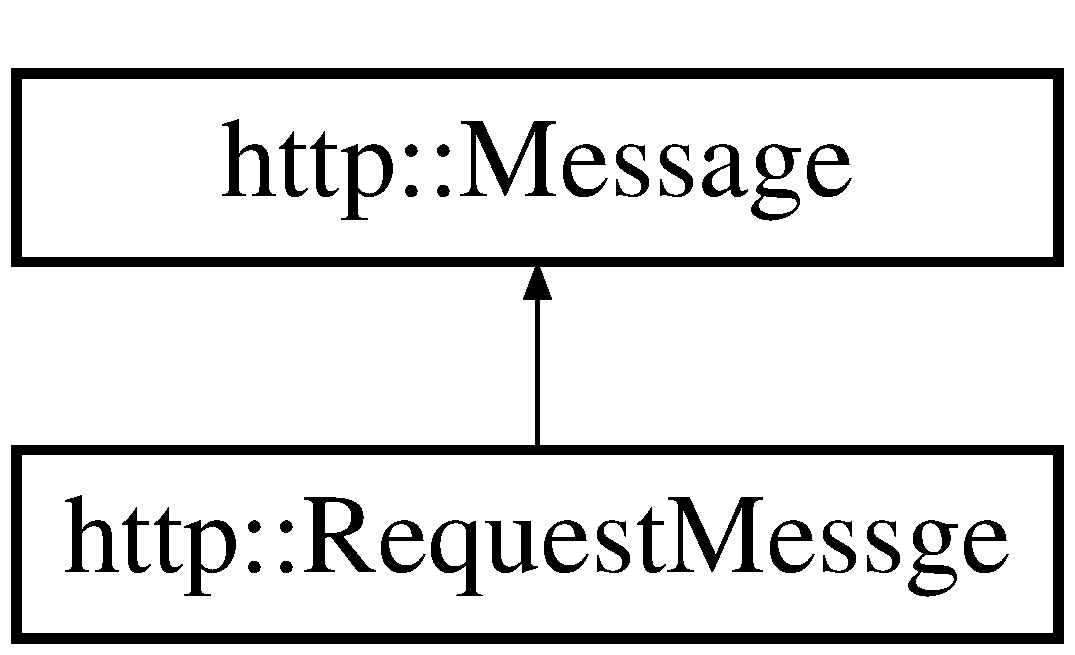
\includegraphics[height=2.000000cm]{classhttp_1_1_request_messge}
\end{center}
\end{figure}
\subsection*{Public 멤버 함수}
\begin{DoxyCompactItemize}
\item 
\hyperlink{classhttp_1_1_request_messge_aa79dcaf03eb6c49010e5df0c75fb3740}{Request\+Messge} (std\+::string msg)
\begin{DoxyCompactList}\small\item\em H\+T\+TP 요청 메세지의 문자열을 입력 받아 \hyperlink{classhttp_1_1_request_messge}{Request\+Messge} 를 만드는 생성자 \end{DoxyCompactList}\item 
\hyperlink{classhttp_1_1_request_messge_a8b9e3bc54bc34d1ec19cf4253057444b}{Request\+Messge} (\hyperlink{structhttp_1_1_request_line}{Request\+Line} request\+Line, \hyperlink{structhttp_1_1_header_line}{Header\+Line} header\+Line\mbox{[}$\,$\mbox{]}, int \hyperlink{classhttp_1_1_message_abf4fab93257b3d37930ed20627f1c061}{header\+Size}, std\+::string content)
\begin{DoxyCompactList}\small\item\em H\+T\+TP 요청 메세지의 첫줄, 파싱된 \hyperlink{structhttp_1_1_header_line}{Header\+Line} , Body를 이용하여 \hyperlink{classhttp_1_1_request_messge}{Request\+Messge} 를 만드는 생성자 \end{DoxyCompactList}\item 
\hyperlink{structhttp_1_1_request_line}{Request\+Line} \hyperlink{classhttp_1_1_request_messge_a6a9c5ce3a93c6949241527d315f4bb17}{get\+Request\+Line} ()
\begin{DoxyCompactList}\small\item\em H\+T\+TP 요청 메세지의 요청 라인을 불러오는 메소드 \end{DoxyCompactList}\end{DoxyCompactItemize}
\subsection*{추가로 상속된 멤버들}


\subsection{상세한 설명}
H\+T\+TP 요청 메시지 

Http.\+hpp 파일의 152 번째 라인에서 정의되었습니다.



\subsection{생성자 \& 소멸자 문서화}
\mbox{\Hypertarget{classhttp_1_1_request_messge_aa79dcaf03eb6c49010e5df0c75fb3740}\label{classhttp_1_1_request_messge_aa79dcaf03eb6c49010e5df0c75fb3740}} 
\index{http\+::\+Request\+Messge@{http\+::\+Request\+Messge}!Request\+Messge@{Request\+Messge}}
\index{Request\+Messge@{Request\+Messge}!http\+::\+Request\+Messge@{http\+::\+Request\+Messge}}
\subsubsection{\texorpdfstring{Request\+Messge()}{RequestMessge()}\hspace{0.1cm}{\footnotesize\ttfamily [1/2]}}
{\footnotesize\ttfamily http\+::\+Request\+Messge\+::\+Request\+Messge (\begin{DoxyParamCaption}\item[{std\+::string}]{msg }\end{DoxyParamCaption})}



H\+T\+TP 요청 메세지의 문자열을 입력 받아 \hyperlink{classhttp_1_1_request_messge}{Request\+Messge} 를 만드는 생성자 

이 함수는 편의를 제공하기 위해 오버로드된 멤버 함수입니다. 위의 함수와 틀린 점은 단지 받아들이는 아규먼트(argument)가 다르다는 것입니다. 
\begin{DoxyParams}{매개변수}
{\em msg} & H\+T\+TP 요청 메세지의 문자열 \\
\hline
\end{DoxyParams}


Http.\+cpp 파일의 151 번째 라인에서 정의되었습니다.

\mbox{\Hypertarget{classhttp_1_1_request_messge_a8b9e3bc54bc34d1ec19cf4253057444b}\label{classhttp_1_1_request_messge_a8b9e3bc54bc34d1ec19cf4253057444b}} 
\index{http\+::\+Request\+Messge@{http\+::\+Request\+Messge}!Request\+Messge@{Request\+Messge}}
\index{Request\+Messge@{Request\+Messge}!http\+::\+Request\+Messge@{http\+::\+Request\+Messge}}
\subsubsection{\texorpdfstring{Request\+Messge()}{RequestMessge()}\hspace{0.1cm}{\footnotesize\ttfamily [2/2]}}
{\footnotesize\ttfamily http\+::\+Request\+Messge\+::\+Request\+Messge (\begin{DoxyParamCaption}\item[{\hyperlink{structhttp_1_1_request_line}{Request\+Line}}]{request\+Line,  }\item[{\hyperlink{structhttp_1_1_header_line}{Header\+Line}}]{header\+Line\mbox{[}$\,$\mbox{]},  }\item[{int}]{header\+Size,  }\item[{std\+::string}]{content }\end{DoxyParamCaption})}



H\+T\+TP 요청 메세지의 첫줄, 파싱된 \hyperlink{structhttp_1_1_header_line}{Header\+Line} , Body를 이용하여 \hyperlink{classhttp_1_1_request_messge}{Request\+Messge} 를 만드는 생성자 

이 함수는 편의를 제공하기 위해 오버로드된 멤버 함수입니다. 위의 함수와 틀린 점은 단지 받아들이는 아규먼트(argument)가 다르다는 것입니다. 
\begin{DoxyParams}{매개변수}
{\em request\+Line} & H\+T\+TP 요청 메세지의 상태 라인 \\
\hline
{\em header\+Line} & H\+T\+TP 요청 메세지의 헤더 라인들 \\
\hline
{\em header\+Size} & 헤더 라인의 갯수 \\
\hline
{\em content} & H\+T\+TP 요청 메세지의 Body \\
\hline
\end{DoxyParams}


Http.\+cpp 파일의 154 번째 라인에서 정의되었습니다.



\subsection{멤버 함수 문서화}
\mbox{\Hypertarget{classhttp_1_1_request_messge_a6a9c5ce3a93c6949241527d315f4bb17}\label{classhttp_1_1_request_messge_a6a9c5ce3a93c6949241527d315f4bb17}} 
\index{http\+::\+Request\+Messge@{http\+::\+Request\+Messge}!get\+Request\+Line@{get\+Request\+Line}}
\index{get\+Request\+Line@{get\+Request\+Line}!http\+::\+Request\+Messge@{http\+::\+Request\+Messge}}
\subsubsection{\texorpdfstring{get\+Request\+Line()}{getRequestLine()}}
{\footnotesize\ttfamily \hyperlink{structhttp_1_1_request_line}{http\+::\+Request\+Line} http\+::\+Request\+Messge\+::get\+Request\+Line (\begin{DoxyParamCaption}{ }\end{DoxyParamCaption})}



H\+T\+TP 요청 메세지의 요청 라인을 불러오는 메소드 

\begin{DoxyReturn}{반환값}
H\+T\+TP 요청 메세지의 요청 라인 
\end{DoxyReturn}


Http.\+cpp 파일의 164 번째 라인에서 정의되었습니다.



이 클래스에 대한 문서화 페이지는 다음의 파일들로부터 생성되었습니다.\+:\begin{DoxyCompactItemize}
\item 
Network/Http.\+hpp\item 
Network/Http.\+cpp\end{DoxyCompactItemize}

\hypertarget{classhttp_1_1_response_messge}{}\section{http\+:\+:Response\+Messge 클래스 참조}
\label{classhttp_1_1_response_messge}\index{http\+::\+Response\+Messge@{http\+::\+Response\+Messge}}


H\+T\+TP 응답 메시지  




{\ttfamily \#include $<$Http.\+hpp$>$}

http\+:\+:Response\+Messge에 대한 상속 다이어그램 \+: \begin{figure}[H]
\begin{center}
\leavevmode
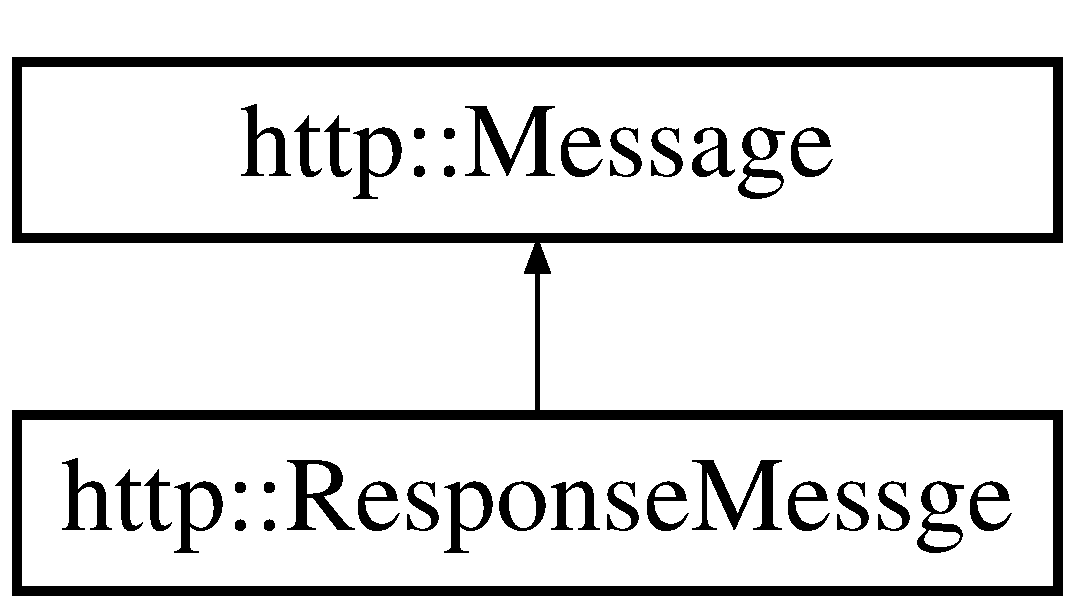
\includegraphics[height=2.000000cm]{classhttp_1_1_response_messge}
\end{center}
\end{figure}
\subsection*{Public 멤버 함수}
\begin{DoxyCompactItemize}
\item 
\hyperlink{classhttp_1_1_response_messge_a20f120ead2d600fc033c3f5ce3d5174e}{Response\+Messge} (std\+::string msg)
\begin{DoxyCompactList}\small\item\em H\+T\+TP 응답 메세지의 문자열을 입력 받아 Response\+Message 를 만드는 생성자 \end{DoxyCompactList}\item 
\hyperlink{classhttp_1_1_response_messge_a278fe12044ee4b4d69b75b3bf6dbe652}{Response\+Messge} (\hyperlink{structhttp_1_1_status_line}{Status\+Line} status\+Code, \hyperlink{structhttp_1_1_header_line}{Header\+Line} header\+Line\mbox{[}$\,$\mbox{]}, int \hyperlink{classhttp_1_1_message_abf4fab93257b3d37930ed20627f1c061}{header\+Size}, std\+::string content)
\begin{DoxyCompactList}\small\item\em H\+T\+TP 응답 메세지의 첫줄, 파싱된 \hyperlink{structhttp_1_1_header_line}{Header\+Line} , Body를 이용하여 Response\+Message 를 만드는 생성자 \end{DoxyCompactList}\item 
\hyperlink{structhttp_1_1_status_line}{Status\+Line} \hyperlink{classhttp_1_1_response_messge_a1be9d3205a0b413828f336c094be4c86}{get\+Status\+Line} ()
\begin{DoxyCompactList}\small\item\em H\+T\+TP 응답 메세지의 상태 라인을 불러오는 메소드 \end{DoxyCompactList}\end{DoxyCompactItemize}
\subsection*{추가로 상속된 멤버들}


\subsection{상세한 설명}
H\+T\+TP 응답 메시지 

Http.\+hpp 파일의 120 번째 라인에서 정의되었습니다.



\subsection{생성자 \& 소멸자 문서화}
\mbox{\Hypertarget{classhttp_1_1_response_messge_a20f120ead2d600fc033c3f5ce3d5174e}\label{classhttp_1_1_response_messge_a20f120ead2d600fc033c3f5ce3d5174e}} 
\index{http\+::\+Response\+Messge@{http\+::\+Response\+Messge}!Response\+Messge@{Response\+Messge}}
\index{Response\+Messge@{Response\+Messge}!http\+::\+Response\+Messge@{http\+::\+Response\+Messge}}
\subsubsection{\texorpdfstring{Response\+Messge()}{ResponseMessge()}\hspace{0.1cm}{\footnotesize\ttfamily [1/2]}}
{\footnotesize\ttfamily http\+::\+Response\+Messge\+::\+Response\+Messge (\begin{DoxyParamCaption}\item[{std\+::string}]{msg }\end{DoxyParamCaption})}



H\+T\+TP 응답 메세지의 문자열을 입력 받아 Response\+Message 를 만드는 생성자 

이 함수는 편의를 제공하기 위해 오버로드된 멤버 함수입니다. 위의 함수와 틀린 점은 단지 받아들이는 아규먼트(argument)가 다르다는 것입니다. 
\begin{DoxyParams}{매개변수}
{\em msg} & H\+T\+TP 응답 메세지의 문자열 \\
\hline
\end{DoxyParams}


Http.\+cpp 파일의 129 번째 라인에서 정의되었습니다.

\mbox{\Hypertarget{classhttp_1_1_response_messge_a278fe12044ee4b4d69b75b3bf6dbe652}\label{classhttp_1_1_response_messge_a278fe12044ee4b4d69b75b3bf6dbe652}} 
\index{http\+::\+Response\+Messge@{http\+::\+Response\+Messge}!Response\+Messge@{Response\+Messge}}
\index{Response\+Messge@{Response\+Messge}!http\+::\+Response\+Messge@{http\+::\+Response\+Messge}}
\subsubsection{\texorpdfstring{Response\+Messge()}{ResponseMessge()}\hspace{0.1cm}{\footnotesize\ttfamily [2/2]}}
{\footnotesize\ttfamily http\+::\+Response\+Messge\+::\+Response\+Messge (\begin{DoxyParamCaption}\item[{\hyperlink{structhttp_1_1_status_line}{Status\+Line}}]{status\+Code,  }\item[{\hyperlink{structhttp_1_1_header_line}{Header\+Line}}]{header\+Line\mbox{[}$\,$\mbox{]},  }\item[{int}]{header\+Size,  }\item[{std\+::string}]{content }\end{DoxyParamCaption})}



H\+T\+TP 응답 메세지의 첫줄, 파싱된 \hyperlink{structhttp_1_1_header_line}{Header\+Line} , Body를 이용하여 Response\+Message 를 만드는 생성자 

이 함수는 편의를 제공하기 위해 오버로드된 멤버 함수입니다. 위의 함수와 틀린 점은 단지 받아들이는 아규먼트(argument)가 다르다는 것입니다. 
\begin{DoxyParams}{매개변수}
{\em status\+Code} & H\+T\+TP 응답 메세지의 상태 라인 \\
\hline
{\em header\+Line} & H\+T\+TP 응답 메세지의 헤더 라인들 \\
\hline
{\em header\+Size} & 헤더 라인의 갯수 \\
\hline
{\em content} & H\+T\+TP 응답 메세지의 Body \\
\hline
\end{DoxyParams}


Http.\+cpp 파일의 133 번째 라인에서 정의되었습니다.



\subsection{멤버 함수 문서화}
\mbox{\Hypertarget{classhttp_1_1_response_messge_a1be9d3205a0b413828f336c094be4c86}\label{classhttp_1_1_response_messge_a1be9d3205a0b413828f336c094be4c86}} 
\index{http\+::\+Response\+Messge@{http\+::\+Response\+Messge}!get\+Status\+Line@{get\+Status\+Line}}
\index{get\+Status\+Line@{get\+Status\+Line}!http\+::\+Response\+Messge@{http\+::\+Response\+Messge}}
\subsubsection{\texorpdfstring{get\+Status\+Line()}{getStatusLine()}}
{\footnotesize\ttfamily \hyperlink{structhttp_1_1_status_line}{http\+::\+Status\+Line} http\+::\+Response\+Messge\+::get\+Status\+Line (\begin{DoxyParamCaption}{ }\end{DoxyParamCaption})}



H\+T\+TP 응답 메세지의 상태 라인을 불러오는 메소드 

\begin{DoxyReturn}{반환값}
H\+T\+TP 응답 메세지의 상태 라인 
\end{DoxyReturn}


Http.\+cpp 파일의 143 번째 라인에서 정의되었습니다.



이 클래스에 대한 문서화 페이지는 다음의 파일들로부터 생성되었습니다.\+:\begin{DoxyCompactItemize}
\item 
Network/Http.\+hpp\item 
Network/Http.\+cpp\end{DoxyCompactItemize}

\hypertarget{classsock_1_1_server_socket}{}\section{sock\+:\+:Server\+Socket 클래스 참조}
\label{classsock_1_1_server_socket}\index{sock\+::\+Server\+Socket@{sock\+::\+Server\+Socket}}


서버 소켓  




{\ttfamily \#include $<$Socket.\+hpp$>$}

sock\+:\+:Server\+Socket에 대한 상속 다이어그램 \+: \begin{figure}[H]
\begin{center}
\leavevmode
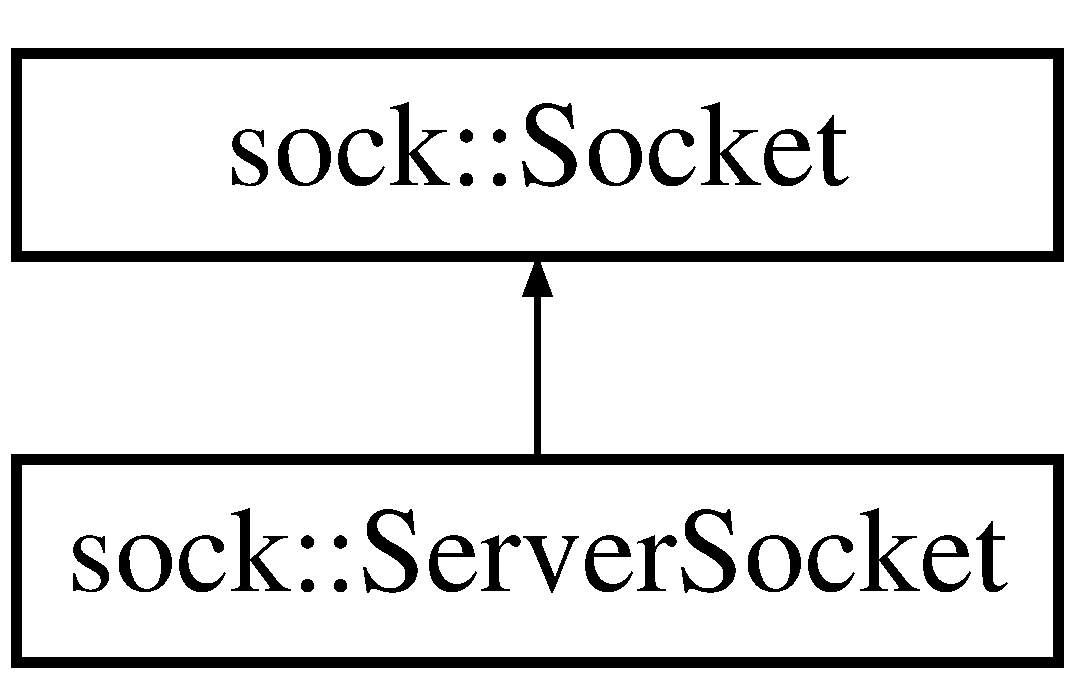
\includegraphics[height=2.000000cm]{classsock_1_1_server_socket}
\end{center}
\end{figure}
\subsection*{Public 멤버 함수}
\begin{DoxyCompactItemize}
\item 
bool \hyperlink{classsock_1_1_server_socket_acaf072e165087c2a2cba2d1f078d8750}{create} ()
\begin{DoxyCompactList}\small\item\em 서버 소켓을 create 하는 메소드 \end{DoxyCompactList}\item 
bool \hyperlink{classsock_1_1_server_socket_a70e23f56e41228cbf43afe7702519f45}{bind} (const int port)
\begin{DoxyCompactList}\small\item\em 서버 소켓을 bind 하는 메소드 \end{DoxyCompactList}\item 
bool \hyperlink{classsock_1_1_server_socket_a3b3431968400296b8b7f9a73dd7c27bc}{listen} ()
\begin{DoxyCompactList}\small\item\em 서버 소켓을 listen 하는 메소드 \end{DoxyCompactList}\item 
bool \hyperlink{classsock_1_1_server_socket_add433570d6d808d667e2f2b5c24a5dd1}{accept} (\hyperlink{classsock_1_1_socket}{Socket} $\ast$client\+Socket)
\begin{DoxyCompactList}\small\item\em 클라이언트 소켓을 accept 하는 메소드 \end{DoxyCompactList}\end{DoxyCompactItemize}
\subsection*{추가로 상속된 멤버들}


\subsection{상세한 설명}
서버 소켓 

Socket.\+hpp 파일의 102 번째 라인에서 정의되었습니다.



\subsection{멤버 함수 문서화}
\mbox{\Hypertarget{classsock_1_1_server_socket_add433570d6d808d667e2f2b5c24a5dd1}\label{classsock_1_1_server_socket_add433570d6d808d667e2f2b5c24a5dd1}} 
\index{sock\+::\+Server\+Socket@{sock\+::\+Server\+Socket}!accept@{accept}}
\index{accept@{accept}!sock\+::\+Server\+Socket@{sock\+::\+Server\+Socket}}
\subsubsection{\texorpdfstring{accept()}{accept()}}
{\footnotesize\ttfamily bool sock\+::\+Server\+Socket\+::accept (\begin{DoxyParamCaption}\item[{\hyperlink{classsock_1_1_socket}{Socket} $\ast$}]{client\+Socket }\end{DoxyParamCaption})}



클라이언트 소켓을 accept 하는 메소드 


\begin{DoxyParams}{매개변수}
{\em client\+Socket} & accept 할 클라이언트의 소켓 \\
\hline
\end{DoxyParams}
\begin{DoxyReturn}{반환값}
성공 시 true 그렇지 않으면 false 
\end{DoxyReturn}


Socket.\+cpp 파일의 146 번째 라인에서 정의되었습니다.

\mbox{\Hypertarget{classsock_1_1_server_socket_a70e23f56e41228cbf43afe7702519f45}\label{classsock_1_1_server_socket_a70e23f56e41228cbf43afe7702519f45}} 
\index{sock\+::\+Server\+Socket@{sock\+::\+Server\+Socket}!bind@{bind}}
\index{bind@{bind}!sock\+::\+Server\+Socket@{sock\+::\+Server\+Socket}}
\subsubsection{\texorpdfstring{bind()}{bind()}}
{\footnotesize\ttfamily bool sock\+::\+Server\+Socket\+::bind (\begin{DoxyParamCaption}\item[{const int}]{port }\end{DoxyParamCaption})}



서버 소켓을 bind 하는 메소드 


\begin{DoxyParams}{매개변수}
{\em port} & port \\
\hline
\end{DoxyParams}
\begin{DoxyReturn}{반환값}
성공 시 true 그렇지 않으면 false 
\end{DoxyReturn}


Socket.\+cpp 파일의 116 번째 라인에서 정의되었습니다.

\mbox{\Hypertarget{classsock_1_1_server_socket_acaf072e165087c2a2cba2d1f078d8750}\label{classsock_1_1_server_socket_acaf072e165087c2a2cba2d1f078d8750}} 
\index{sock\+::\+Server\+Socket@{sock\+::\+Server\+Socket}!create@{create}}
\index{create@{create}!sock\+::\+Server\+Socket@{sock\+::\+Server\+Socket}}
\subsubsection{\texorpdfstring{create()}{create()}}
{\footnotesize\ttfamily bool sock\+::\+Server\+Socket\+::create (\begin{DoxyParamCaption}{ }\end{DoxyParamCaption})}



서버 소켓을 create 하는 메소드 

\begin{DoxyReturn}{반환값}
성공 시 true 그렇지 않으면 false 
\end{DoxyReturn}


Socket.\+cpp 파일의 100 번째 라인에서 정의되었습니다.

\mbox{\Hypertarget{classsock_1_1_server_socket_a3b3431968400296b8b7f9a73dd7c27bc}\label{classsock_1_1_server_socket_a3b3431968400296b8b7f9a73dd7c27bc}} 
\index{sock\+::\+Server\+Socket@{sock\+::\+Server\+Socket}!listen@{listen}}
\index{listen@{listen}!sock\+::\+Server\+Socket@{sock\+::\+Server\+Socket}}
\subsubsection{\texorpdfstring{listen()}{listen()}}
{\footnotesize\ttfamily bool sock\+::\+Server\+Socket\+::listen (\begin{DoxyParamCaption}{ }\end{DoxyParamCaption})}



서버 소켓을 listen 하는 메소드 

\begin{DoxyReturn}{반환값}
성공 시 true 그렇지 않으면 false 
\end{DoxyReturn}


Socket.\+cpp 파일의 133 번째 라인에서 정의되었습니다.



이 클래스에 대한 문서화 페이지는 다음의 파일들로부터 생성되었습니다.\+:\begin{DoxyCompactItemize}
\item 
Network/Socket.\+hpp\item 
Network/Socket.\+cpp\end{DoxyCompactItemize}

\hypertarget{classsock_1_1_socket}{}\section{sock\+:\+:Socket 클래스 참조}
\label{classsock_1_1_socket}\index{sock\+::\+Socket@{sock\+::\+Socket}}


소켓 클래스  




{\ttfamily \#include $<$Socket.\+hpp$>$}

sock\+:\+:Socket에 대한 상속 다이어그램 \+: \begin{figure}[H]
\begin{center}
\leavevmode
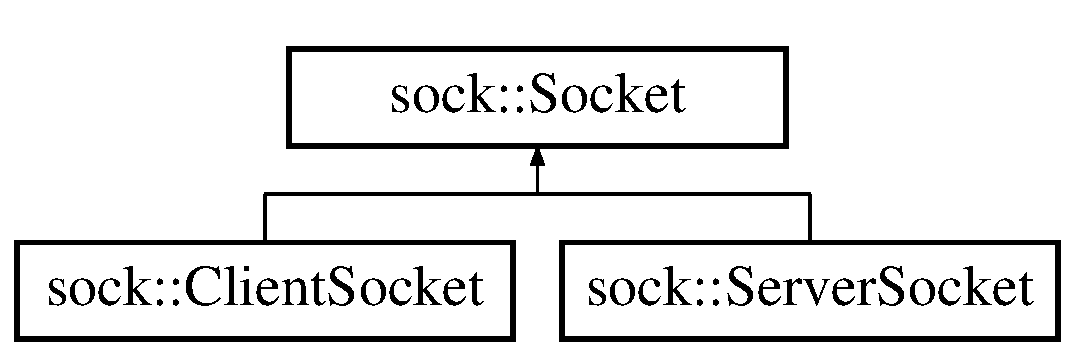
\includegraphics[height=2.000000cm]{classsock_1_1_socket}
\end{center}
\end{figure}
\subsection*{Public 멤버 함수}
\begin{DoxyCompactItemize}
\item 
\hyperlink{classsock_1_1_socket_a9983ebd97b8f79d3e4c67fca05811dcb}{Socket} ()
\begin{DoxyCompactList}\small\item\em \hyperlink{classsock_1_1_socket}{Socket} 클래스를 초기화하는 생성자 \end{DoxyCompactList}\item 
\hyperlink{classsock_1_1_socket_a570a3285956f8923f490f9203a6d1d8f}{Socket} (int \hyperlink{classsock_1_1_socket_a01040adb35eea5ad276090b9db112f4a}{sock})
\begin{DoxyCompactList}\small\item\em 파일 기술자를 통해 \hyperlink{classsock_1_1_socket}{Socket} 클래스를 초기화하는 생성자 \end{DoxyCompactList}\item 
\mbox{\Hypertarget{classsock_1_1_socket_a2efd63baf692cd9e466da55139f74838}\label{classsock_1_1_socket_a2efd63baf692cd9e466da55139f74838}} 
\hyperlink{classsock_1_1_socket_a2efd63baf692cd9e466da55139f74838}{$\sim$\+Socket} ()
\begin{DoxyCompactList}\small\item\em \hyperlink{classsock_1_1_socket}{Socket} 클래스의 소멸자 \end{DoxyCompactList}\item 
bool \hyperlink{classsock_1_1_socket_a1d980395d1e06e4b9e1c5c65a2220a0a}{send} (const std\+::string data)
\begin{DoxyCompactList}\small\item\em 소켓을 통해 데이터를 보내는 메소드 \end{DoxyCompactList}\item 
int \hyperlink{classsock_1_1_socket_aa52c41c177bd1f7fe785d32d46f60b9f}{recv} (std\+::string $\ast$data)
\begin{DoxyCompactList}\small\item\em 소켓으로 부터 데이터를 받는 메소드 \end{DoxyCompactList}\item 
bool \hyperlink{classsock_1_1_socket_a448363328243c35f7899761381cac1df}{is\+Valid} ()
\begin{DoxyCompactList}\small\item\em 소켓이 올바른지 검사하는 메소드 \end{DoxyCompactList}\item 
void \hyperlink{classsock_1_1_socket_a908007148692a4a8dfa6a339b679b8a8}{set\+\_\+non\+\_\+blocking} (bool b)
\begin{DoxyCompactList}\small\item\em nonblocking I/O 설정 \end{DoxyCompactList}\end{DoxyCompactItemize}
\subsection*{정적 Public 속성}
\begin{DoxyCompactItemize}
\item 
\mbox{\Hypertarget{classsock_1_1_socket_ac1b998d21d786e8a40019079581cbe5a}\label{classsock_1_1_socket_ac1b998d21d786e8a40019079581cbe5a}} 
static const int \hyperlink{classsock_1_1_socket_ac1b998d21d786e8a40019079581cbe5a}{M\+A\+X\+H\+O\+S\+T\+N\+A\+ME} = 200
\begin{DoxyCompactList}\small\item\em hostname 의 최대 길이 \end{DoxyCompactList}\item 
\mbox{\Hypertarget{classsock_1_1_socket_a9f25b6bda1196c775ef4d71db6d74d1c}\label{classsock_1_1_socket_a9f25b6bda1196c775ef4d71db6d74d1c}} 
static const int \hyperlink{classsock_1_1_socket_a9f25b6bda1196c775ef4d71db6d74d1c}{M\+A\+X\+C\+O\+N\+N\+E\+C\+T\+I\+O\+NS} = 5
\begin{DoxyCompactList}\small\item\em 최대 연결 가능한 연결 수 \end{DoxyCompactList}\item 
\mbox{\Hypertarget{classsock_1_1_socket_a01030a5c8737ce91eb7d03ffb8793bad}\label{classsock_1_1_socket_a01030a5c8737ce91eb7d03ffb8793bad}} 
static const int \hyperlink{classsock_1_1_socket_a01030a5c8737ce91eb7d03ffb8793bad}{M\+A\+X\+R\+E\+CV} = 500
\begin{DoxyCompactList}\small\item\em recv 시 받는 버퍼의 크기 \end{DoxyCompactList}\end{DoxyCompactItemize}
\subsection*{Protected 속성}
\begin{DoxyCompactItemize}
\item 
\mbox{\Hypertarget{classsock_1_1_socket_a3a0ac1ff8d4b3ace6fc85c75f8174299}\label{classsock_1_1_socket_a3a0ac1ff8d4b3ace6fc85c75f8174299}} 
sockaddr\+\_\+in $\ast$ \hyperlink{classsock_1_1_socket_a3a0ac1ff8d4b3ace6fc85c75f8174299}{addr}
\begin{DoxyCompactList}\small\item\em 소켓 주소를 지정하는 구조체 \end{DoxyCompactList}\item 
\mbox{\Hypertarget{classsock_1_1_socket_a01040adb35eea5ad276090b9db112f4a}\label{classsock_1_1_socket_a01040adb35eea5ad276090b9db112f4a}} 
int \hyperlink{classsock_1_1_socket_a01040adb35eea5ad276090b9db112f4a}{sock}
\begin{DoxyCompactList}\small\item\em 소켓 파일 기술자 \end{DoxyCompactList}\end{DoxyCompactItemize}


\subsection{상세한 설명}
소켓 클래스 

Socket.\+hpp 파일의 23 번째 라인에서 정의되었습니다.



\subsection{생성자 \& 소멸자 문서화}
\mbox{\Hypertarget{classsock_1_1_socket_a9983ebd97b8f79d3e4c67fca05811dcb}\label{classsock_1_1_socket_a9983ebd97b8f79d3e4c67fca05811dcb}} 
\index{sock\+::\+Socket@{sock\+::\+Socket}!Socket@{Socket}}
\index{Socket@{Socket}!sock\+::\+Socket@{sock\+::\+Socket}}
\subsubsection{\texorpdfstring{Socket()}{Socket()}\hspace{0.1cm}{\footnotesize\ttfamily [1/2]}}
{\footnotesize\ttfamily sock\+::\+Socket\+::\+Socket (\begin{DoxyParamCaption}{ }\end{DoxyParamCaption})}



\hyperlink{classsock_1_1_socket}{Socket} 클래스를 초기화하는 생성자 

이 함수는 편의를 제공하기 위해 오버로드된 멤버 함수입니다. 위의 함수와 틀린 점은 단지 받아들이는 아규먼트(argument)가 다르다는 것입니다. 

Socket.\+cpp 파일의 15 번째 라인에서 정의되었습니다.

\mbox{\Hypertarget{classsock_1_1_socket_a570a3285956f8923f490f9203a6d1d8f}\label{classsock_1_1_socket_a570a3285956f8923f490f9203a6d1d8f}} 
\index{sock\+::\+Socket@{sock\+::\+Socket}!Socket@{Socket}}
\index{Socket@{Socket}!sock\+::\+Socket@{sock\+::\+Socket}}
\subsubsection{\texorpdfstring{Socket()}{Socket()}\hspace{0.1cm}{\footnotesize\ttfamily [2/2]}}
{\footnotesize\ttfamily sock\+::\+Socket\+::\+Socket (\begin{DoxyParamCaption}\item[{int}]{sock }\end{DoxyParamCaption})}



파일 기술자를 통해 \hyperlink{classsock_1_1_socket}{Socket} 클래스를 초기화하는 생성자 

이 함수는 편의를 제공하기 위해 오버로드된 멤버 함수입니다. 위의 함수와 틀린 점은 단지 받아들이는 아규먼트(argument)가 다르다는 것입니다. 
\begin{DoxyParams}{매개변수}
{\em sock} & 초기화할 파일 기술자 \\
\hline
\end{DoxyParams}


Socket.\+cpp 파일의 27 번째 라인에서 정의되었습니다.



\subsection{멤버 함수 문서화}
\mbox{\Hypertarget{classsock_1_1_socket_a448363328243c35f7899761381cac1df}\label{classsock_1_1_socket_a448363328243c35f7899761381cac1df}} 
\index{sock\+::\+Socket@{sock\+::\+Socket}!is\+Valid@{is\+Valid}}
\index{is\+Valid@{is\+Valid}!sock\+::\+Socket@{sock\+::\+Socket}}
\subsubsection{\texorpdfstring{is\+Valid()}{isValid()}}
{\footnotesize\ttfamily bool sock\+::\+Socket\+::is\+Valid (\begin{DoxyParamCaption}{ }\end{DoxyParamCaption})}



소켓이 올바른지 검사하는 메소드 

\begin{DoxyReturn}{반환값}
성공 시 true 그렇지 않으면 false 
\end{DoxyReturn}


Socket.\+cpp 파일의 41 번째 라인에서 정의되었습니다.

\mbox{\Hypertarget{classsock_1_1_socket_aa52c41c177bd1f7fe785d32d46f60b9f}\label{classsock_1_1_socket_aa52c41c177bd1f7fe785d32d46f60b9f}} 
\index{sock\+::\+Socket@{sock\+::\+Socket}!recv@{recv}}
\index{recv@{recv}!sock\+::\+Socket@{sock\+::\+Socket}}
\subsubsection{\texorpdfstring{recv()}{recv()}}
{\footnotesize\ttfamily int sock\+::\+Socket\+::recv (\begin{DoxyParamCaption}\item[{std\+::string $\ast$}]{data }\end{DoxyParamCaption})}



소켓으로 부터 데이터를 받는 메소드 


\begin{DoxyParams}{매개변수}
{\em data} & 소켓으로 부터 받은 데이터 \\
\hline
\end{DoxyParams}
\begin{DoxyReturn}{반환값}
성공 시 받은 데이터의 크기을 반환, 실패 시 -\/1을 반환 
\end{DoxyReturn}


Socket.\+cpp 파일의 57 번째 라인에서 정의되었습니다.

\mbox{\Hypertarget{classsock_1_1_socket_a1d980395d1e06e4b9e1c5c65a2220a0a}\label{classsock_1_1_socket_a1d980395d1e06e4b9e1c5c65a2220a0a}} 
\index{sock\+::\+Socket@{sock\+::\+Socket}!send@{send}}
\index{send@{send}!sock\+::\+Socket@{sock\+::\+Socket}}
\subsubsection{\texorpdfstring{send()}{send()}}
{\footnotesize\ttfamily bool sock\+::\+Socket\+::send (\begin{DoxyParamCaption}\item[{const std\+::string}]{data }\end{DoxyParamCaption})}



소켓을 통해 데이터를 보내는 메소드 


\begin{DoxyParams}{매개변수}
{\em data} & 소켓을 통해 보낼 데이터 \\
\hline
\end{DoxyParams}
\begin{DoxyReturn}{반환값}
성공 시 true 그렇지 않으면 false 
\end{DoxyReturn}


Socket.\+cpp 파일의 47 번째 라인에서 정의되었습니다.

\mbox{\Hypertarget{classsock_1_1_socket_a908007148692a4a8dfa6a339b679b8a8}\label{classsock_1_1_socket_a908007148692a4a8dfa6a339b679b8a8}} 
\index{sock\+::\+Socket@{sock\+::\+Socket}!set\+\_\+non\+\_\+blocking@{set\+\_\+non\+\_\+blocking}}
\index{set\+\_\+non\+\_\+blocking@{set\+\_\+non\+\_\+blocking}!sock\+::\+Socket@{sock\+::\+Socket}}
\subsubsection{\texorpdfstring{set\+\_\+non\+\_\+blocking()}{set\_non\_blocking()}}
{\footnotesize\ttfamily void sock\+::\+Socket\+::set\+\_\+non\+\_\+blocking (\begin{DoxyParamCaption}\item[{bool}]{b }\end{DoxyParamCaption})}



nonblocking I/O 설정 


\begin{DoxyParams}{매개변수}
{\em b} & true 시 nonblocking false 시 blocking \\
\hline
\end{DoxyParams}


Socket.\+cpp 파일의 81 번째 라인에서 정의되었습니다.



이 클래스에 대한 문서화 페이지는 다음의 파일들로부터 생성되었습니다.\+:\begin{DoxyCompactItemize}
\item 
Network/Socket.\+hpp\item 
Network/Socket.\+cpp\end{DoxyCompactItemize}

\hypertarget{structhttp_1_1_status_line}{}\section{http\+:\+:Status\+Line 구조체 참조}
\label{structhttp_1_1_status_line}\index{http\+::\+Status\+Line@{http\+::\+Status\+Line}}


\hyperlink{classhttp_1_1_response_messge}{Response\+Messge} 의 상태 라인  




{\ttfamily \#include $<$Http.\+hpp$>$}

\subsection*{Public 속성}
\begin{DoxyCompactItemize}
\item 
\mbox{\Hypertarget{structhttp_1_1_status_line_af3500800ad3ac685b19763d5e60b6353}\label{structhttp_1_1_status_line_af3500800ad3ac685b19763d5e60b6353}} 
std\+::string \hyperlink{structhttp_1_1_status_line_af3500800ad3ac685b19763d5e60b6353}{version}
\begin{DoxyCompactList}\small\item\em H\+T\+TP 버전 \end{DoxyCompactList}\item 
\mbox{\Hypertarget{structhttp_1_1_status_line_acfd9752d4b62330a390f17f5d011fcd2}\label{structhttp_1_1_status_line_acfd9752d4b62330a390f17f5d011fcd2}} 
std\+::string \hyperlink{structhttp_1_1_status_line_acfd9752d4b62330a390f17f5d011fcd2}{status}
\begin{DoxyCompactList}\small\item\em 상태 코드 \end{DoxyCompactList}\item 
\mbox{\Hypertarget{structhttp_1_1_status_line_a9f49c5c1cc247c2a85ed717870bfc844}\label{structhttp_1_1_status_line_a9f49c5c1cc247c2a85ed717870bfc844}} 
std\+::string \hyperlink{structhttp_1_1_status_line_a9f49c5c1cc247c2a85ed717870bfc844}{message}
\begin{DoxyCompactList}\small\item\em 상태 메세지 \end{DoxyCompactList}\end{DoxyCompactItemize}


\subsection{상세한 설명}
\hyperlink{classhttp_1_1_response_messge}{Response\+Messge} 의 상태 라인 

Http.\+hpp 파일의 29 번째 라인에서 정의되었습니다.



이 구조체에 대한 문서화 페이지는 다음의 파일로부터 생성되었습니다.\+:\begin{DoxyCompactItemize}
\item 
Network/Http.\+hpp\end{DoxyCompactItemize}

\hypertarget{class_svm}{}\section{Svm 클래스 참조}
\label{class_svm}\index{Svm@{Svm}}


Support Vector Machines을 다루기 위한 클래스  




{\ttfamily \#include $<$Svm.\+hpp$>$}

\subsection*{Public 타입}
\begin{DoxyCompactItemize}
\item 
enum \hyperlink{class_svm_a479f12db422de0a4c4d46900ee154928}{M\+O\+DE} \{ \hyperlink{class_svm_a479f12db422de0a4c4d46900ee154928aeb592b07b32a90ab0b49f8912740562a}{R\+E\+A\+D\+DT} = 0b00, 
\hyperlink{class_svm_a479f12db422de0a4c4d46900ee154928a97cff7c5edfa23dfdb9047aa49acb5ad}{C\+O\+L\+L\+E\+CT} = 0b01, 
\hyperlink{class_svm_a479f12db422de0a4c4d46900ee154928acfc63391c47b89218369105e12b992fb}{W\+R\+I\+T\+E\+DT} = 0b11
 \}\begin{DoxyCompactList}\small\item\em 훈련 데이터를 다룰 방법 \end{DoxyCompactList}
\end{DoxyCompactItemize}
\subsection*{Public 멤버 함수}
\begin{DoxyCompactItemize}
\item 
\hyperlink{class_svm_a762af972a037686ea80d9896905f57ed}{Svm} (const int mode)
\begin{DoxyCompactList}\small\item\em \hyperlink{class_svm}{Svm} 초기화 \end{DoxyCompactList}\item 
float \hyperlink{class_svm_ad157df6a49f7380a99232e5b8fa6b63e}{predict} (const cv\+::\+Mat \&img)
\begin{DoxyCompactList}\small\item\em 입력된 Sample이 훈련된 Support Vector Machines의해 예측된 결과를 출력 \end{DoxyCompactList}\end{DoxyCompactItemize}
\subsection*{Private 멤버 함수}
\begin{DoxyCompactItemize}
\item 
\mbox{\Hypertarget{class_svm_a1b18e97fffb268f9cfe91152f7e96298}\label{class_svm_a1b18e97fffb268f9cfe91152f7e96298}} 
void \hyperlink{class_svm_a1b18e97fffb268f9cfe91152f7e96298}{collect\+Train\+Images} ()
\begin{DoxyCompactList}\small\item\em trainimage에서 훈련 데이터 불러오기 \textquotesingle{}trainimage\textquotesingle{}에 경로에서 모든 이미지 파일을 읽어들여 훈련 데이터를 생성한다. \end{DoxyCompactList}\item 
void \hyperlink{class_svm_a303d7fad50a71154c8201883db777ca1}{write\+Traindata} (const std\+::string fn)
\begin{DoxyCompactList}\small\item\em 훈련 데이터를 File System에 Json 파일로 쓰기 \end{DoxyCompactList}\item 
void \hyperlink{class_svm_afb95b76fa494604abcd022c5948fb728}{read\+Traindata} (const std\+::string fn)
\begin{DoxyCompactList}\small\item\em 훈련 데이터를 File System에서 Json 파일로부터 불러오기 \end{DoxyCompactList}\end{DoxyCompactItemize}
\subsection*{Private 속성}
\begin{DoxyCompactItemize}
\item 
\mbox{\Hypertarget{class_svm_ac4e8ba994bfa1f66d17ef3b0fa2d856c}\label{class_svm_ac4e8ba994bfa1f66d17ef3b0fa2d856c}} 
cv\+::\+Ptr$<$ cv\+::ml\+::\+S\+VM $>$ \hyperlink{class_svm_ac4e8ba994bfa1f66d17ef3b0fa2d856c}{svm}
\begin{DoxyCompactList}\small\item\em Support Vector Machines \end{DoxyCompactList}\item 
\mbox{\Hypertarget{class_svm_a76663f6a5d1baa4185887451aed8e577}\label{class_svm_a76663f6a5d1baa4185887451aed8e577}} 
cv\+::\+Mat \hyperlink{class_svm_a76663f6a5d1baa4185887451aed8e577}{classes}
\begin{DoxyCompactList}\small\item\em training\+Data와 연관된 출력될 vectors \end{DoxyCompactList}\item 
\mbox{\Hypertarget{class_svm_a29ecb047ff1b1dc376b60e9e4bf11b37}\label{class_svm_a29ecb047ff1b1dc376b60e9e4bf11b37}} 
cv\+::\+Mat \hyperlink{class_svm_a29ecb047ff1b1dc376b60e9e4bf11b37}{training\+Data}
\begin{DoxyCompactList}\small\item\em 훈련을 위한 Samples \end{DoxyCompactList}\end{DoxyCompactItemize}


\subsection{상세한 설명}
Support Vector Machines을 다루기 위한 클래스 

Svm.\+hpp 파일의 10 번째 라인에서 정의되었습니다.



\subsection{멤버 열거형 문서화}
\mbox{\Hypertarget{class_svm_a479f12db422de0a4c4d46900ee154928}\label{class_svm_a479f12db422de0a4c4d46900ee154928}} 
\index{Svm@{Svm}!M\+O\+DE@{M\+O\+DE}}
\index{M\+O\+DE@{M\+O\+DE}!Svm@{Svm}}
\subsubsection{\texorpdfstring{M\+O\+DE}{MODE}}
{\footnotesize\ttfamily enum \hyperlink{class_svm_a479f12db422de0a4c4d46900ee154928}{Svm\+::\+M\+O\+DE}}



훈련 데이터를 다룰 방법 

\begin{DoxyEnumFields}{열거형 멤버}
\raisebox{\heightof{T}}[0pt][0pt]{\index{R\+E\+A\+D\+DT@{R\+E\+A\+D\+DT}!Svm@{Svm}}\index{Svm@{Svm}!R\+E\+A\+D\+DT@{R\+E\+A\+D\+DT}}}\mbox{\Hypertarget{class_svm_a479f12db422de0a4c4d46900ee154928aeb592b07b32a90ab0b49f8912740562a}\label{class_svm_a479f12db422de0a4c4d46900ee154928aeb592b07b32a90ab0b49f8912740562a}} 
R\+E\+A\+D\+DT&Json File에서 읽기 \begin{DoxySeeAlso}{참고}
\hyperlink{class_svm_afb95b76fa494604abcd022c5948fb728}{read\+Traindata} 
\end{DoxySeeAlso}
\\
\hline

\raisebox{\heightof{T}}[0pt][0pt]{\index{C\+O\+L\+L\+E\+CT@{C\+O\+L\+L\+E\+CT}!Svm@{Svm}}\index{Svm@{Svm}!C\+O\+L\+L\+E\+CT@{C\+O\+L\+L\+E\+CT}}}\mbox{\Hypertarget{class_svm_a479f12db422de0a4c4d46900ee154928a97cff7c5edfa23dfdb9047aa49acb5ad}\label{class_svm_a479f12db422de0a4c4d46900ee154928a97cff7c5edfa23dfdb9047aa49acb5ad}} 
C\+O\+L\+L\+E\+CT&trainimage에서 읽기 \begin{DoxySeeAlso}{참고}
\hyperlink{class_svm_a1b18e97fffb268f9cfe91152f7e96298}{collect\+Train\+Images} 
\end{DoxySeeAlso}
\\
\hline

\raisebox{\heightof{T}}[0pt][0pt]{\index{W\+R\+I\+T\+E\+DT@{W\+R\+I\+T\+E\+DT}!Svm@{Svm}}\index{Svm@{Svm}!W\+R\+I\+T\+E\+DT@{W\+R\+I\+T\+E\+DT}}}\mbox{\Hypertarget{class_svm_a479f12db422de0a4c4d46900ee154928acfc63391c47b89218369105e12b992fb}\label{class_svm_a479f12db422de0a4c4d46900ee154928acfc63391c47b89218369105e12b992fb}} 
W\+R\+I\+T\+E\+DT&Json File로 쓰기 \begin{DoxySeeAlso}{참고}
\hyperlink{class_svm_a303d7fad50a71154c8201883db777ca1}{write\+Traindata} 
\end{DoxySeeAlso}
\\
\hline

\end{DoxyEnumFields}


Svm.\+hpp 파일의 38 번째 라인에서 정의되었습니다.



\subsection{생성자 \& 소멸자 문서화}
\mbox{\Hypertarget{class_svm_a762af972a037686ea80d9896905f57ed}\label{class_svm_a762af972a037686ea80d9896905f57ed}} 
\index{Svm@{Svm}!Svm@{Svm}}
\index{Svm@{Svm}!Svm@{Svm}}
\subsubsection{\texorpdfstring{Svm()}{Svm()}}
{\footnotesize\ttfamily Svm\+::\+Svm (\begin{DoxyParamCaption}\item[{const int}]{mode }\end{DoxyParamCaption})}



\hyperlink{class_svm}{Svm} 초기화 


\begin{DoxyParams}{매개변수}
{\em mode} & \hyperlink{class_svm}{Svm} 모드 설정 \\
\hline
\end{DoxyParams}
\begin{DoxySeeAlso}{참고}
\hyperlink{class_svm_a479f12db422de0a4c4d46900ee154928}{M\+O\+DE} 
\end{DoxySeeAlso}


Svm.\+cpp 파일의 8 번째 라인에서 정의되었습니다.



\subsection{멤버 함수 문서화}
\mbox{\Hypertarget{class_svm_ad157df6a49f7380a99232e5b8fa6b63e}\label{class_svm_ad157df6a49f7380a99232e5b8fa6b63e}} 
\index{Svm@{Svm}!predict@{predict}}
\index{predict@{predict}!Svm@{Svm}}
\subsubsection{\texorpdfstring{predict()}{predict()}}
{\footnotesize\ttfamily float Svm\+::predict (\begin{DoxyParamCaption}\item[{const cv\+::\+Mat \&}]{img }\end{DoxyParamCaption})}



입력된 Sample이 훈련된 Support Vector Machines의해 예측된 결과를 출력 


\begin{DoxyParams}{매개변수}
{\em img} & 입력할 Sample \\
\hline
\end{DoxyParams}
\begin{DoxyReturn}{반환값}
Svm을 통해 0 $\sim$ 1로 분류된 결과 
\end{DoxyReturn}


Svm.\+cpp 파일의 61 번째 라인에서 정의되었습니다.

\mbox{\Hypertarget{class_svm_afb95b76fa494604abcd022c5948fb728}\label{class_svm_afb95b76fa494604abcd022c5948fb728}} 
\index{Svm@{Svm}!read\+Traindata@{read\+Traindata}}
\index{read\+Traindata@{read\+Traindata}!Svm@{Svm}}
\subsubsection{\texorpdfstring{read\+Traindata()}{readTraindata()}}
{\footnotesize\ttfamily void Svm\+::read\+Traindata (\begin{DoxyParamCaption}\item[{const std\+::string}]{fn }\end{DoxyParamCaption})\hspace{0.3cm}{\ttfamily [private]}}



훈련 데이터를 File System에서 Json 파일로부터 불러오기 


\begin{DoxyParams}{매개변수}
{\em fn} & Josn 파일의 경로 \\
\hline
\end{DoxyParams}


Svm.\+cpp 파일의 65 번째 라인에서 정의되었습니다.

\mbox{\Hypertarget{class_svm_a303d7fad50a71154c8201883db777ca1}\label{class_svm_a303d7fad50a71154c8201883db777ca1}} 
\index{Svm@{Svm}!write\+Traindata@{write\+Traindata}}
\index{write\+Traindata@{write\+Traindata}!Svm@{Svm}}
\subsubsection{\texorpdfstring{write\+Traindata()}{writeTraindata()}}
{\footnotesize\ttfamily void Svm\+::write\+Traindata (\begin{DoxyParamCaption}\item[{const std\+::string}]{fn }\end{DoxyParamCaption})\hspace{0.3cm}{\ttfamily [private]}}



훈련 데이터를 File System에 Json 파일로 쓰기 


\begin{DoxyParams}{매개변수}
{\em fn} & Josn 파일의 경로 \\
\hline
\end{DoxyParams}


Svm.\+cpp 파일의 81 번째 라인에서 정의되었습니다.



이 클래스에 대한 문서화 페이지는 다음의 파일들로부터 생성되었습니다.\+:\begin{DoxyCompactItemize}
\item 
Opencv/Svm.\+hpp\item 
Opencv/Svm.\+cpp\end{DoxyCompactItemize}

\hypertarget{class_s_v_m_trainer}{}\section{S\+V\+M\+Trainer 클래스 참조}
\label{class_s_v_m_trainer}\index{S\+V\+M\+Trainer@{S\+V\+M\+Trainer}}


\hyperlink{class_svm_a1b18e97fffb268f9cfe91152f7e96298}{Svm\+::collect\+Train\+Images} 실행 시 필요한 image를 생성하는 클래스  




{\ttfamily \#include $<$Svm.\+hpp$>$}

\subsection*{Public 멤버 함수}
\begin{DoxyCompactItemize}
\item 
\mbox{\Hypertarget{class_s_v_m_trainer_a2109fcf47792fe25ac12e14368c775bb}\label{class_s_v_m_trainer_a2109fcf47792fe25ac12e14368c775bb}} 
\hyperlink{class_s_v_m_trainer_a2109fcf47792fe25ac12e14368c775bb}{S\+V\+M\+Trainer} ()
\begin{DoxyCompactList}\small\item\em \hyperlink{class_s_v_m_trainer}{S\+V\+M\+Trainer} 초기화 \end{DoxyCompactList}\item 
void \hyperlink{class_s_v_m_trainer_a60f3eb8020709966c067246c98b610c4}{train} (const cv\+::\+Mat \&sample)
\begin{DoxyCompactList}\small\item\em \hyperlink{class_svm}{Svm} 클래스에서 참조할 이미지를 File System에 쓰기 \end{DoxyCompactList}\end{DoxyCompactItemize}
\subsection*{Private 속성}
\begin{DoxyCompactItemize}
\item 
\mbox{\Hypertarget{class_s_v_m_trainer_ad7ac47f8d93360bac934cf399f37b967}\label{class_s_v_m_trainer_ad7ac47f8d93360bac934cf399f37b967}} 
int \hyperlink{class_s_v_m_trainer_ad7ac47f8d93360bac934cf399f37b967}{file\+Index}
\begin{DoxyCompactList}\small\item\em File 검색을 위한 Index 변수 \end{DoxyCompactList}\end{DoxyCompactItemize}


\subsection{상세한 설명}
\hyperlink{class_svm_a1b18e97fffb268f9cfe91152f7e96298}{Svm\+::collect\+Train\+Images} 실행 시 필요한 image를 생성하는 클래스 

\subsection{멤버 함수 문서화}
\mbox{\Hypertarget{class_s_v_m_trainer_a60f3eb8020709966c067246c98b610c4}\label{class_s_v_m_trainer_a60f3eb8020709966c067246c98b610c4}} 
\index{S\+V\+M\+Trainer@{S\+V\+M\+Trainer}!train@{train}}
\index{train@{train}!S\+V\+M\+Trainer@{S\+V\+M\+Trainer}}
\subsubsection{\texorpdfstring{train()}{train()}}
{\footnotesize\ttfamily void S\+V\+M\+Trainer\+::train (\begin{DoxyParamCaption}\item[{const cv\+::\+Mat \&}]{sample }\end{DoxyParamCaption})}



\hyperlink{class_svm}{Svm} 클래스에서 참조할 이미지를 File System에 쓰기 


\begin{DoxyParams}{매개변수}
{\em sample} & File System에 쓸 이미지 입력받은 이미지를 \textquotesingle{}Train\+Image\textquotesingle{}경로에 File System로 쓴다. \\
\hline
\end{DoxyParams}


이 클래스에 대한 문서화 페이지는 다음의 파일들로부터 생성되었습니다.\+:\begin{DoxyCompactItemize}
\item 
Opencv/Svm.\+hpp\item 
Opencv/Svm.\+cpp\end{DoxyCompactItemize}

\hypertarget{structprocess_1_1_table}{}\section{process\+:\+:Table 구조체 참조}
\label{structprocess_1_1_table}\index{process\+::\+Table@{process\+::\+Table}}


주차 차량 정보  




{\ttfamily \#include $<$process.\+hpp$>$}

\subsection*{Public 속성}
\begin{DoxyCompactItemize}
\item 
\mbox{\Hypertarget{structprocess_1_1_table_a5cffcdbe502a6165eb806b64ba27fbe0}\label{structprocess_1_1_table_a5cffcdbe502a6165eb806b64ba27fbe0}} 
std\+::string \hyperlink{structprocess_1_1_table_a5cffcdbe502a6165eb806b64ba27fbe0}{plate\+Str} = \char`\"{}\char`\"{}
\begin{DoxyCompactList}\small\item\em 번호판 텍스트 \end{DoxyCompactList}\item 
\mbox{\Hypertarget{structprocess_1_1_table_a930e1f2f75a47d337ad2fab346791c19}\label{structprocess_1_1_table_a930e1f2f75a47d337ad2fab346791c19}} 
int \hyperlink{structprocess_1_1_table_a930e1f2f75a47d337ad2fab346791c19}{match} = 0
\begin{DoxyCompactList}\small\item\em 일치한 횟수 \end{DoxyCompactList}\item 
\mbox{\Hypertarget{structprocess_1_1_table_aefdb336dc1532718fcbf1708a35d9aff}\label{structprocess_1_1_table_aefdb336dc1532718fcbf1708a35d9aff}} 
bool \hyperlink{structprocess_1_1_table_aefdb336dc1532718fcbf1708a35d9aff}{sended} = false
\begin{DoxyCompactList}\small\item\em Sever 전송 여부 \end{DoxyCompactList}\end{DoxyCompactItemize}


\subsection{상세한 설명}
주차 차량 정보 

이 구조체에 대한 문서화 페이지는 다음의 파일로부터 생성되었습니다.\+:\begin{DoxyCompactItemize}
\item 
Opencv/process.\+hpp\end{DoxyCompactItemize}

\hypertarget{class_plate_1_1_text}{}\section{Plate\+:\+:Text 클래스 참조}
\label{class_plate_1_1_text}\index{Plate\+::\+Text@{Plate\+::\+Text}}


텍스트 번호판을 구성하는 텍스트들 중 하나  




{\ttfamily \#include $<$Plate.\+hpp$>$}

\subsection*{Public 멤버 함수}
\begin{DoxyCompactItemize}
\item 
\hyperlink{class_plate_1_1_text_a7d9cc837bb93e89f5b8bd6aee6cd578b}{Text} (const cv\+::\+Mat \&src)
\begin{DoxyCompactList}\small\item\em Text의 이미지 초기화 \end{DoxyCompactList}\item 
cv\+::\+Mat \hyperlink{class_plate_1_1_text_a1fc8fd54d9274fac2740737f7b1e572e}{canonical} (int sample\+Size)
\begin{DoxyCompactList}\small\item\em img를 정규화한 이미지 출력 \end{DoxyCompactList}\end{DoxyCompactItemize}
\subsection*{Public 속성}
\begin{DoxyCompactItemize}
\item 
\mbox{\Hypertarget{class_plate_1_1_text_a29f1e54dfab056697c4634d3763be2c0}\label{class_plate_1_1_text_a29f1e54dfab056697c4634d3763be2c0}} 
cv\+::\+Mat \hyperlink{class_plate_1_1_text_a29f1e54dfab056697c4634d3763be2c0}{img}
\begin{DoxyCompactList}\small\item\em 텍스트를 나타내는 이미지 \end{DoxyCompactList}\end{DoxyCompactItemize}


\subsection{상세한 설명}
텍스트 번호판을 구성하는 텍스트들 중 하나 

\subsection{생성자 \& 소멸자 문서화}
\mbox{\Hypertarget{class_plate_1_1_text_a7d9cc837bb93e89f5b8bd6aee6cd578b}\label{class_plate_1_1_text_a7d9cc837bb93e89f5b8bd6aee6cd578b}} 
\index{Plate\+::\+Text@{Plate\+::\+Text}!Text@{Text}}
\index{Text@{Text}!Plate\+::\+Text@{Plate\+::\+Text}}
\subsubsection{\texorpdfstring{Text()}{Text()}}
{\footnotesize\ttfamily Plate\+::\+Text\+::\+Text (\begin{DoxyParamCaption}\item[{const cv\+::\+Mat \&}]{src }\end{DoxyParamCaption})}



Text의 이미지 초기화 


\begin{DoxyParams}{매개변수}
{\em src} & 초기화 할 이미지 \\
\hline
\end{DoxyParams}


\subsection{멤버 함수 문서화}
\mbox{\Hypertarget{class_plate_1_1_text_a1fc8fd54d9274fac2740737f7b1e572e}\label{class_plate_1_1_text_a1fc8fd54d9274fac2740737f7b1e572e}} 
\index{Plate\+::\+Text@{Plate\+::\+Text}!canonical@{canonical}}
\index{canonical@{canonical}!Plate\+::\+Text@{Plate\+::\+Text}}
\subsubsection{\texorpdfstring{canonical()}{canonical()}}
{\footnotesize\ttfamily Mat Plate\+::\+Text\+::canonical (\begin{DoxyParamCaption}\item[{int}]{sample\+Size }\end{DoxyParamCaption})}



img를 정규화한 이미지 출력 


\begin{DoxyParams}{매개변수}
{\em sample\+Size} & 정규화하기 위한 가로 세로의 크기 \\
\hline
\end{DoxyParams}
\begin{DoxyReturn}{반환값}
정규화된 이미지 
\end{DoxyReturn}


이 클래스에 대한 문서화 페이지는 다음의 파일들로부터 생성되었습니다.\+:\begin{DoxyCompactItemize}
\item 
Opencv/Plate.\+hpp\item 
Opencv/Plate.\+cpp\end{DoxyCompactItemize}

%--- End generated contents ---

% Index
\backmatter
\newpage
\phantomsection
\clearemptydoublepage
\addcontentsline{toc}{chapter}{색인}
\printindex

\end{document}
